\documentclass[10pt handout]{beamer}\usepackage[]{graphicx}\usepackage[]{color}
%% maxwidth is the original width if it is less than linewidth
%% otherwise use linewidth (to make sure the graphics do not exceed the margin)
\makeatletter
\def\maxwidth{ %
  \ifdim\Gin@nat@width>\linewidth
    \linewidth
  \else
    \Gin@nat@width
  \fi
}
\makeatother

\definecolor{fgcolor}{rgb}{0.345, 0.345, 0.345}
\newcommand{\hlnum}[1]{\textcolor[rgb]{0.686,0.059,0.569}{#1}}%
\newcommand{\hlstr}[1]{\textcolor[rgb]{0.192,0.494,0.8}{#1}}%
\newcommand{\hlcom}[1]{\textcolor[rgb]{0.678,0.584,0.686}{\textit{#1}}}%
\newcommand{\hlopt}[1]{\textcolor[rgb]{0,0,0}{#1}}%
\newcommand{\hlstd}[1]{\textcolor[rgb]{0.345,0.345,0.345}{#1}}%
\newcommand{\hlkwa}[1]{\textcolor[rgb]{0.161,0.373,0.58}{\textbf{#1}}}%
\newcommand{\hlkwb}[1]{\textcolor[rgb]{0.69,0.353,0.396}{#1}}%
\newcommand{\hlkwc}[1]{\textcolor[rgb]{0.333,0.667,0.333}{#1}}%
\newcommand{\hlkwd}[1]{\textcolor[rgb]{0.737,0.353,0.396}{\textbf{#1}}}%

\usepackage{framed}
\makeatletter
\newenvironment{kframe}{%
 \def\at@end@of@kframe{}%
 \ifinner\ifhmode%
  \def\at@end@of@kframe{\end{minipage}}%
  \begin{minipage}{\columnwidth}%
 \fi\fi%
 \def\FrameCommand##1{\hskip\@totalleftmargin \hskip-\fboxsep
 \colorbox{shadecolor}{##1}\hskip-\fboxsep
     % There is no \\@totalrightmargin, so:
     \hskip-\linewidth \hskip-\@totalleftmargin \hskip\columnwidth}%
 \MakeFramed {\advance\hsize-\width
   \@totalleftmargin\z@ \linewidth\hsize
   \@setminipage}}%
 {\par\unskip\endMakeFramed%
 \at@end@of@kframe}
\makeatother

\definecolor{shadecolor}{rgb}{.97, .97, .97}
\definecolor{messagecolor}{rgb}{0, 0, 0}
\definecolor{warningcolor}{rgb}{1, 0, 1}
\definecolor{errorcolor}{rgb}{1, 0, 0}
\newenvironment{knitrout}{}{} % an empty environment to be redefined in TeX

\usepackage{alltt}
%% LyX 2.0.5.1 created this file. For more info, see http://www.lyx.org/.
%% Do not edit unless you really know what you are doing.
%%\documentclass[10pt]{beamer}

\usepackage{beamerthemesplit} %// Activate for custom appearance
\usepackage{multicol}
\usepackage{bm}
\usepackage{amsfonts}
\usepackage{amssymb}
\usepackage{natbib}
\usepackage{siunitx}
\DeclareSIUnit\year{yr}
\DeclareSIUnit\carbon{C}

\setbeamertemplate{caption}{\insertcaption} \setbeamertemplate{caption label separator}{}

\newcommand{\red}[1]{{\color[rgb]{1,0,0}#1}}
\newcommand{\blue}[1]{{\color[rgb]{0,0,1}#1}}

\def\colorize<#1>{\alt<#1>{\color{red}}{\color{black}}}

\renewcommand{\vec}[1]{\mathbf{#1}}
\newcommand{\tens}[1]{\mathbf{\mathrm{#1}}}

\newcommand{\E}{\mathbb{E}}
\renewcommand{\P}{\mathbb{P}}
\newcommand{\Exp}{\operatorname{Exp}}
\newcommand{\deriv}[1]{\frac{d}{d #1}}
\newcommand{\intl}{\int\limits}
\newcommand{\FTT}{\operatorname{FTT}}
\newcommand{\BTT}{\operatorname{BTT}}

%\usetheme{Luebeck}
\usetheme[compress]{MPIM}
 \usecolortheme{orchid}
\setcounter{secnumdepth}{3}
\setcounter{tocdepth}{3}
\usepackage{url}
\usepackage[utf8]{inputenc}
\ifx\hypersetup\undefined
  \AtBeginDocument{%
    \hypersetup{unicode=true,pdfusetitle,
 bookmarks=true,bookmarksnumbered=false,bookmarksopen=false,
 breaklinks=false,pdfborder={0 0 0},backref=false,colorlinks=false}
  }
\else
  \hypersetup{unicode=true,pdfusetitle,
 bookmarks=true,bookmarksnumbered=false,bookmarksopen=false,
 breaklinks=false,pdfborder={0 0 0},backref=false,colorlinks=false}
\fi
\usepackage{breakurl}

\makeatletter

%%%%%%%%%%%%%%%%%%%%%%%%%%%%%% LyX specific LaTeX commands.
\providecommand{\LyX}{\texorpdfstring%
  {L\kern-.1667em\lower.25em\hbox{Y}\kern-.125emX\@}
  {LyX}}

%%%%%%%%%%%%%%%%%%%%%%%%%%%%%% Textclass specific LaTeX commands.
 % this default might be overridden by plain title style
 \newcommand\makebeamertitle{\frame{\maketitle}}%
 \AtBeginDocument{
   \let\origtableofcontents=\tableofcontents
   \def\tableofcontents{\@ifnextchar[{\origtableofcontents}{\gobbletableofcontents}}
   \def\gobbletableofcontents#1{\origtableofcontents}
 }
 \def\lyxframeend{} % In case there is a superfluous frame end
 \long\def\lyxframe#1{\@lyxframe#1\@lyxframestop}%
 \def\@lyxframe{\@ifnextchar<{\@@lyxframe}{\@@lyxframe<*>}}%
 \def\@@lyxframe<#1>{\@ifnextchar[{\@@@lyxframe<#1>}{\@@@lyxframe<#1>[]}}
 \def\@@@lyxframe<#1>[{\@ifnextchar<{\@@@@@lyxframe<#1>[}{\@@@@lyxframe<#1>[<*>][}}
 \def\@@@@@lyxframe<#1>[#2]{\@ifnextchar[{\@@@@lyxframe<#1>[#2]}{\@@@@lyxframe<#1>[#2][]}}
 \long\def\@@@@lyxframe<#1>[#2][#3]#4\@lyxframestop#5\lyxframeend{%
   \frame<#1>[#2][#3]{\frametitle{#4}#5}}

%%%%%%%%%%%%%%%%%%%%%%%%%%%%%% User specified LaTeX commands.
%\usetheme{PaloAlto}
%  \usetheme{Warsaw}
%  %\usetheme{default}
  \setbeamercovered{invisible}
\renewcommand{\familydefault}{\sfdefault}


\makeatother

\begin{document}

\bibliographystyle{plainnat}




%\makebeamertitle

\lyxframeend{}
%
%
%\AtBeginSection[] % Do nothing for \section*
{
\begin{frame}<beamer>
\frametitle{}
\tableofcontents[currentsection] % Inhaltsverz. vor jeder Section einblenden
\end{frame}
}
%\mode<presentation>
%{
\title {Pool Models}
\subtitle {An Introduction } % (optional)
%\subtitle {A classification by required and obtainable information} % (optional)
\author {Markus Müller, Holger Metzler, Carlos Sierra}
\makebeamertitle
%%%%%%%%%%%%%%%%%%%%%%%%%%%%%%%%%%%%%%%%%%%%%%%%%%%%%%%%%%%%%%%%%%%%%%%%%%%%%%%%%%%%%%%%%%%%%%%%%%%%%
\begin{frame}
	\begin{itemize}
		\item What are pool models?
		\item Why do we need them?
		\item What can they be used for?
			\begin{itemize}
				\item What is needed?
				\item What can we learn from them?
			\end{itemize}
	\end{itemize}
\end{frame}
%
%%%%%%%%%%%%%%%%%%%%%%%%%%%%%%%%%%%%%%%%%%%%%%%%%%%%%%%%%%%%%%%%%%%%%%%%%%%%%%%%%%%%%%%%%%%%%%%%%%%%%
\begin{frame}
  \titlepage
\end{frame}
\begin{frame}
  \frametitle{Outline}
  \tableofcontents[pausesections]
\end{frame}
%%%%%%%%%%%%%%%%%%%%%%%%%%%%%%%%%%%%%%%%%%%%%%%%%%%%%%%%%%%%%%%%%%%%%%%%%%%%%%%%%%%%%%%%%%%%%%%%%%%%%
%%%%%%%%%%%%%%%%%%%%%%%%%%%%%%%%%%%%%%%%%%%%%%%%%%%%%%%%%%%%%%%%%%%%%%%%%%%%%%%%%%%%%%%%%%%%%%%%%%%%%
\section{Example Applications of Pool Models}
%%%%%%%%%%%%%%%%%%%%%%%%%%%%%%%%%%%%%%%%%%%%%%%%%%%%%%%%%%%%%%%%%%%%%%%%%%%%%%%%%%%%%%%%%%%%%%%%%%%%%
\begin{frame}
  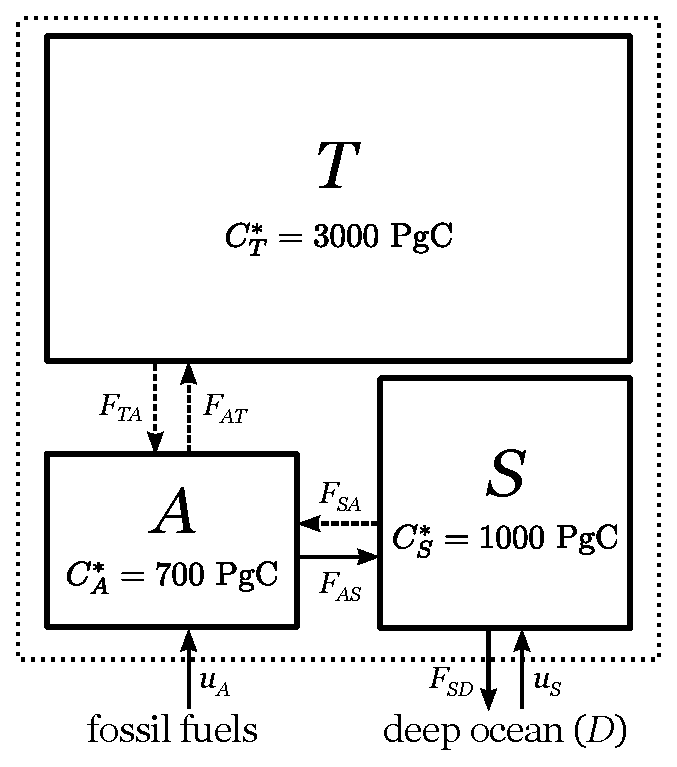
\includegraphics[height=0.9\textheight]{model2.pdf}
\end{frame}

%%%%%%%%%%%%%%%%%%%%%%%%%%%%%%%%%%%%%%%%%%%%%%%%%%%%%%%%%%%%%%%%%%%%%%%%%%%%%%%%%%%%%%%%%%%%%%%%%%%%%
\begin{frame}
	\frametitle{Hydrology Watersheds}
	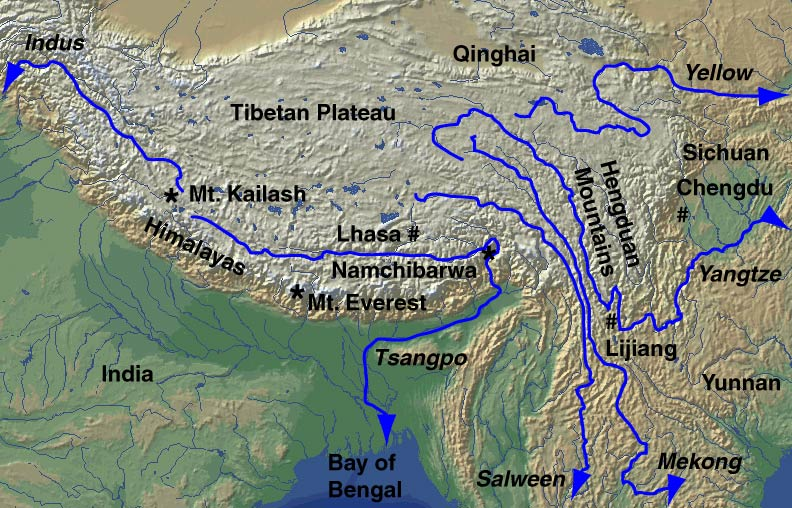
\includegraphics[width=0.9\textwidth]{Watersheds.jpeg}
\end{frame}
%%%%%%%%%%%%%%%%%%%%%%%%%%%%%%%%%%%%%%%%%%%%%%%%%%%%%%%%%%%%%%%%%%%%%%%%%%%%%%%%%%%%%%%%%%%%%%%%%%%%%
\begin{frame}
	\frametitle{Hydrology Catchments}
	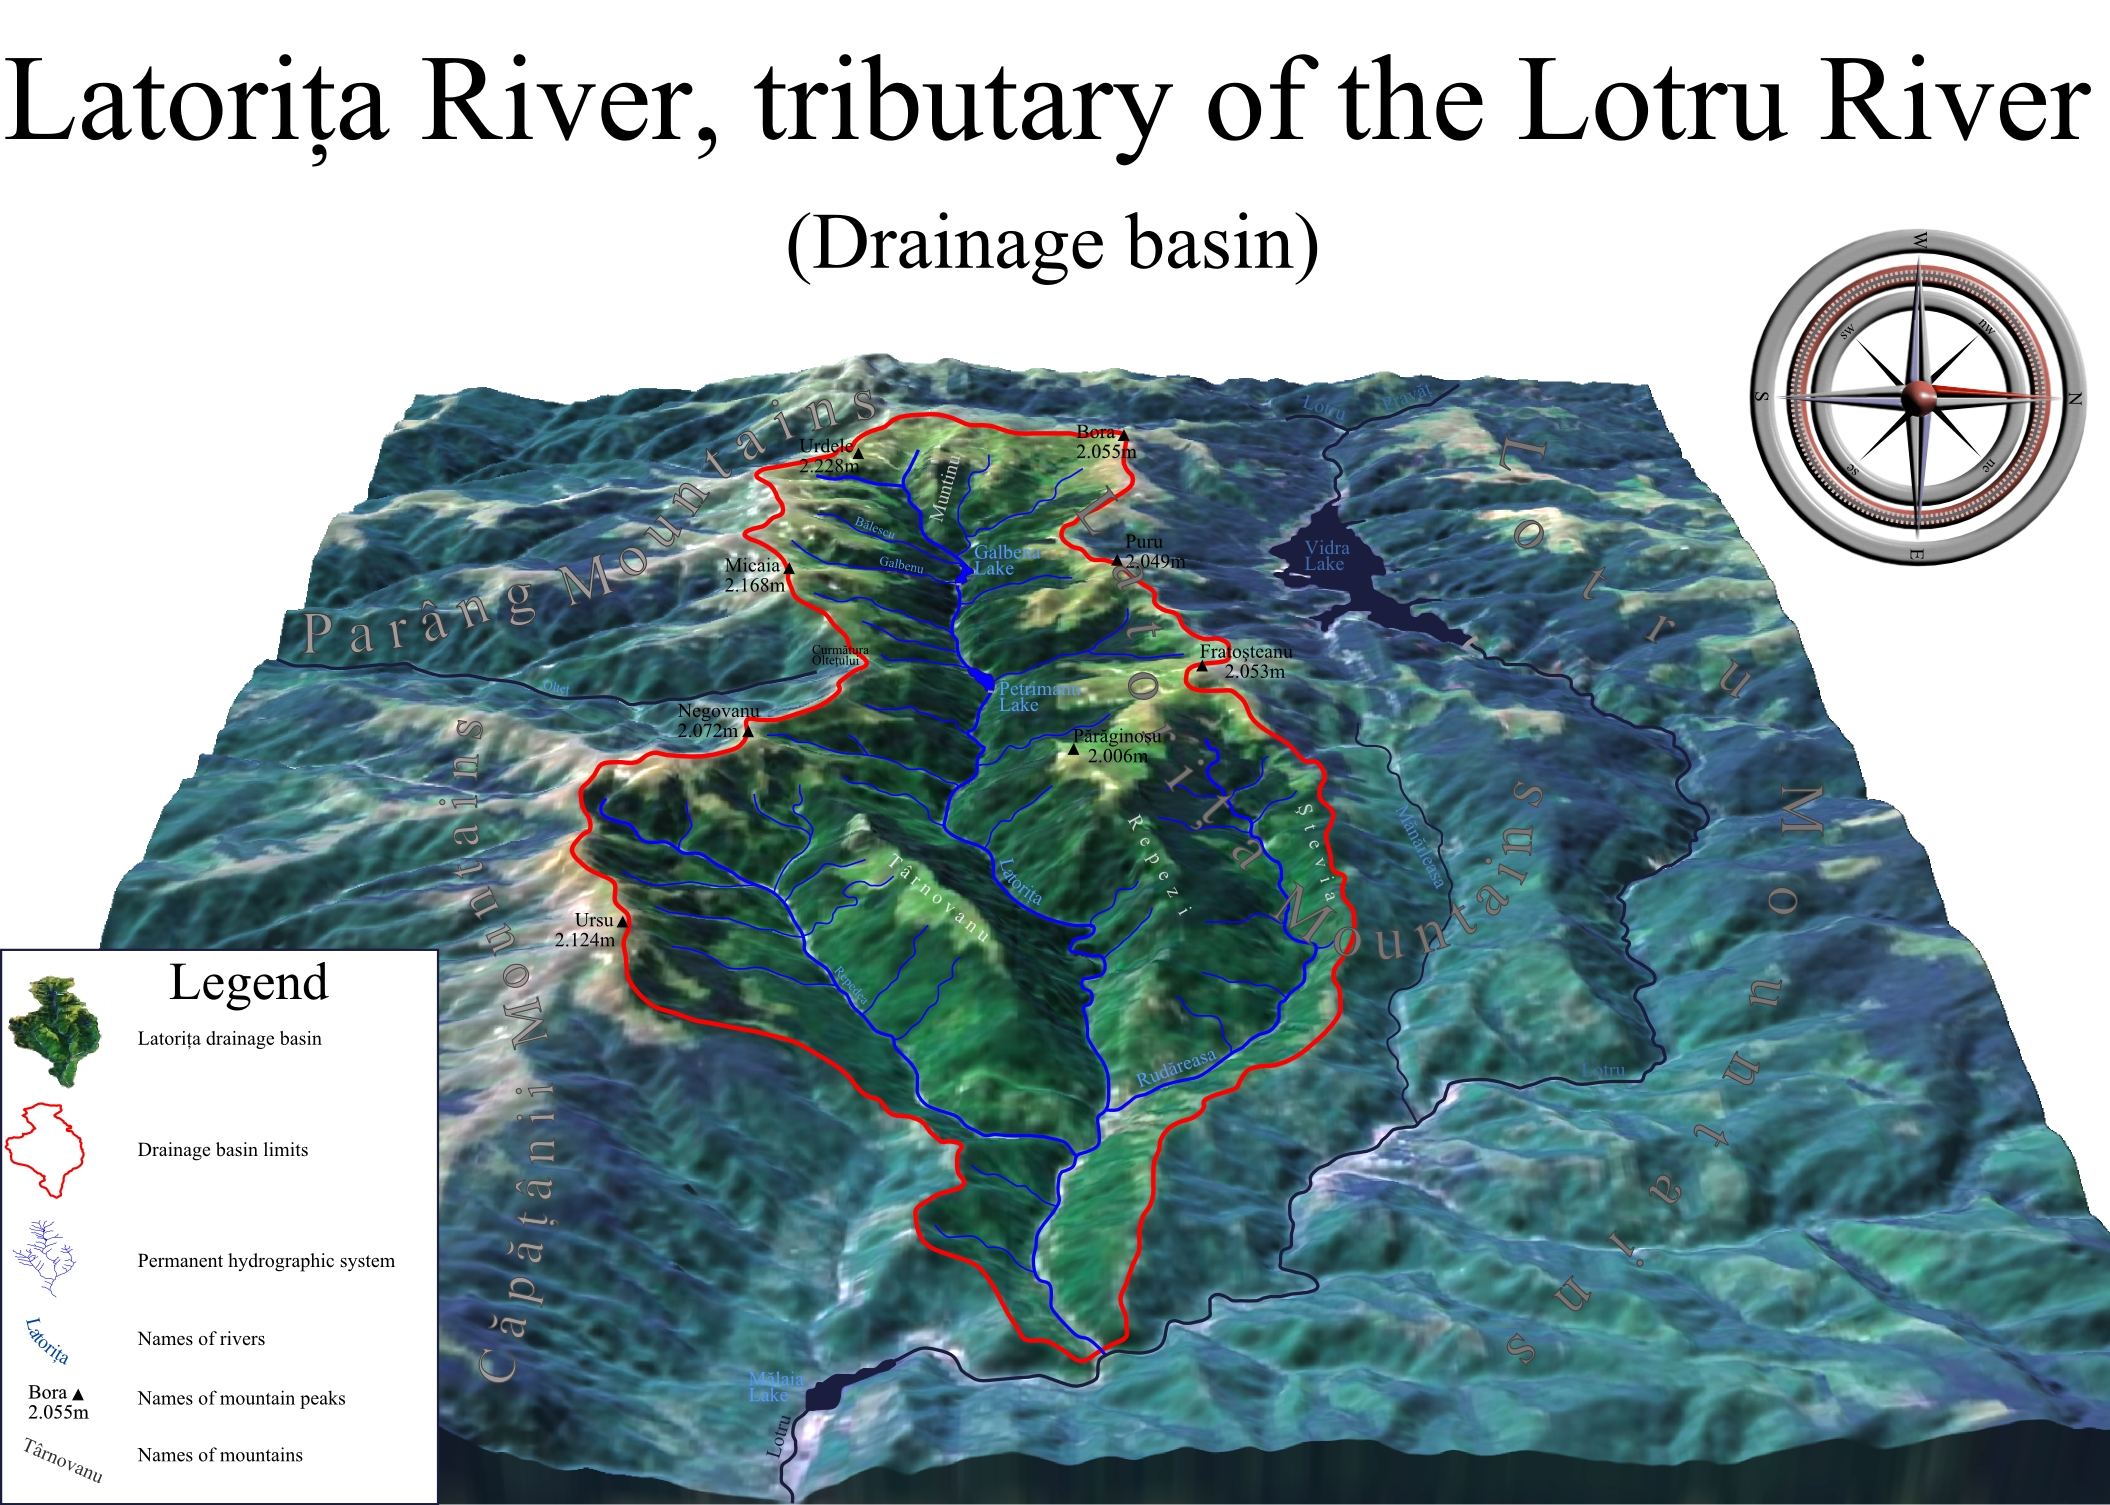
\includegraphics[width=0.9\textwidth]{EN_Bazinul_hidrografic_al_Raului_Latorita,_Romania.jpg}
\end{frame}
%%%%%%%%%%%%%%%%%%%%%%%%%%%%%%%%%%%%%%%%%%%%%%%%%%%%%%%%%%%%%%%%%%%%%%%%%%%%%%%%%%%%%%%%%%%%%%%%%%%%%
%%%%%%%%%%%%%%%%%%%%%%%%%%%%%%%%%%%%%%%%%%%%%%%%%%%%%%%%%%%%%%%%%%%%%%%%%%%%%%%%%%%%%%%%%%%%%%%%%%%%%
\begin{frame}
	\frametitle{Plant Physiology/ Carbon allocation}
	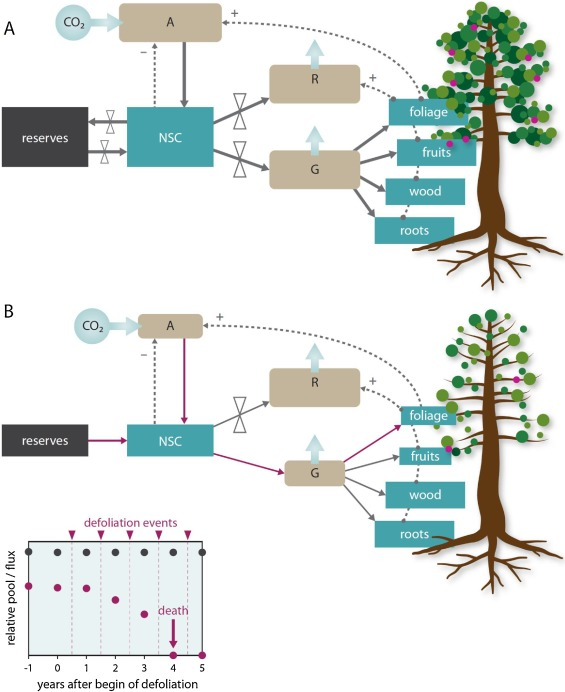
\includegraphics[height=0.9\textheight]{CarbonAllocation.jpg}
	\cite{Hartmann2018EEB}
\end{frame}
%%%%%%%%%%%%%%%%%%%%%%%%%%%%%%%%%%%%%%%%%%%%%%%%%%%%%%%%%%%%%%%%%%%%%%%%%%%%%%%%%%%%%%%%%%%%%%%%%%%%%
\begin{frame}
	\frametitle{Organic Matter Decomposition / Soil Models}
	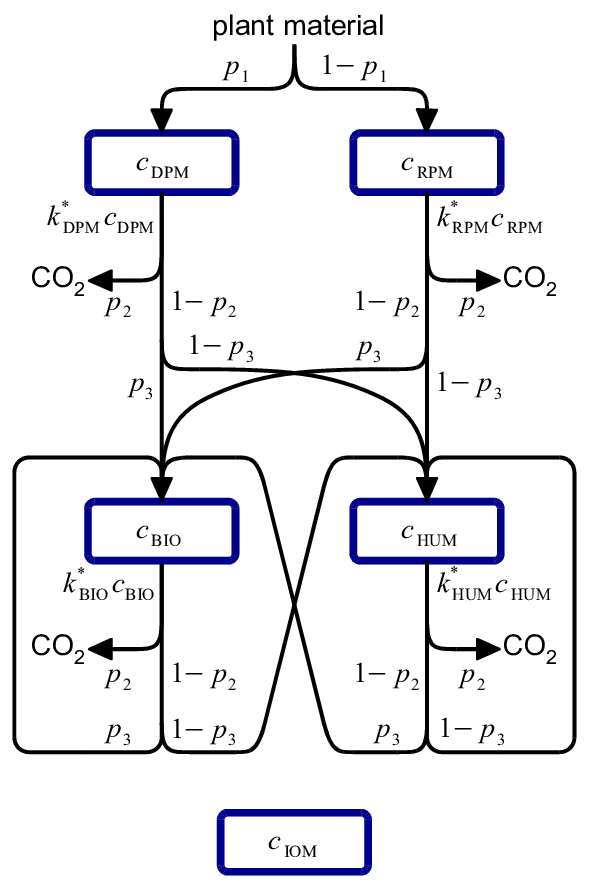
\includegraphics[width=0.35\textwidth]{RothC.png}
	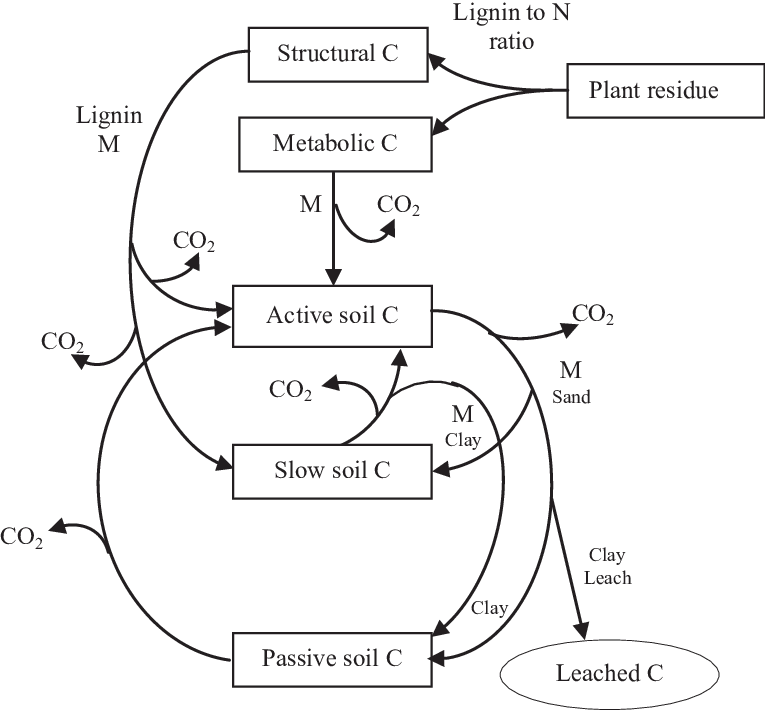
\includegraphics[width=0.55\textwidth]{Century.png}
\end{frame}
%%%%%%%%%%%%%%%%%%%%%%%%%%%%%%%%%%%%%%%%%%%%%%%%%%%%%%%%%%%%%%%%%%%%%%%%%%%%%%%%%%%%%%%%%%%%%%%%%%%%%
\begin{frame}
	\frametitle{Ecosystem Models}
	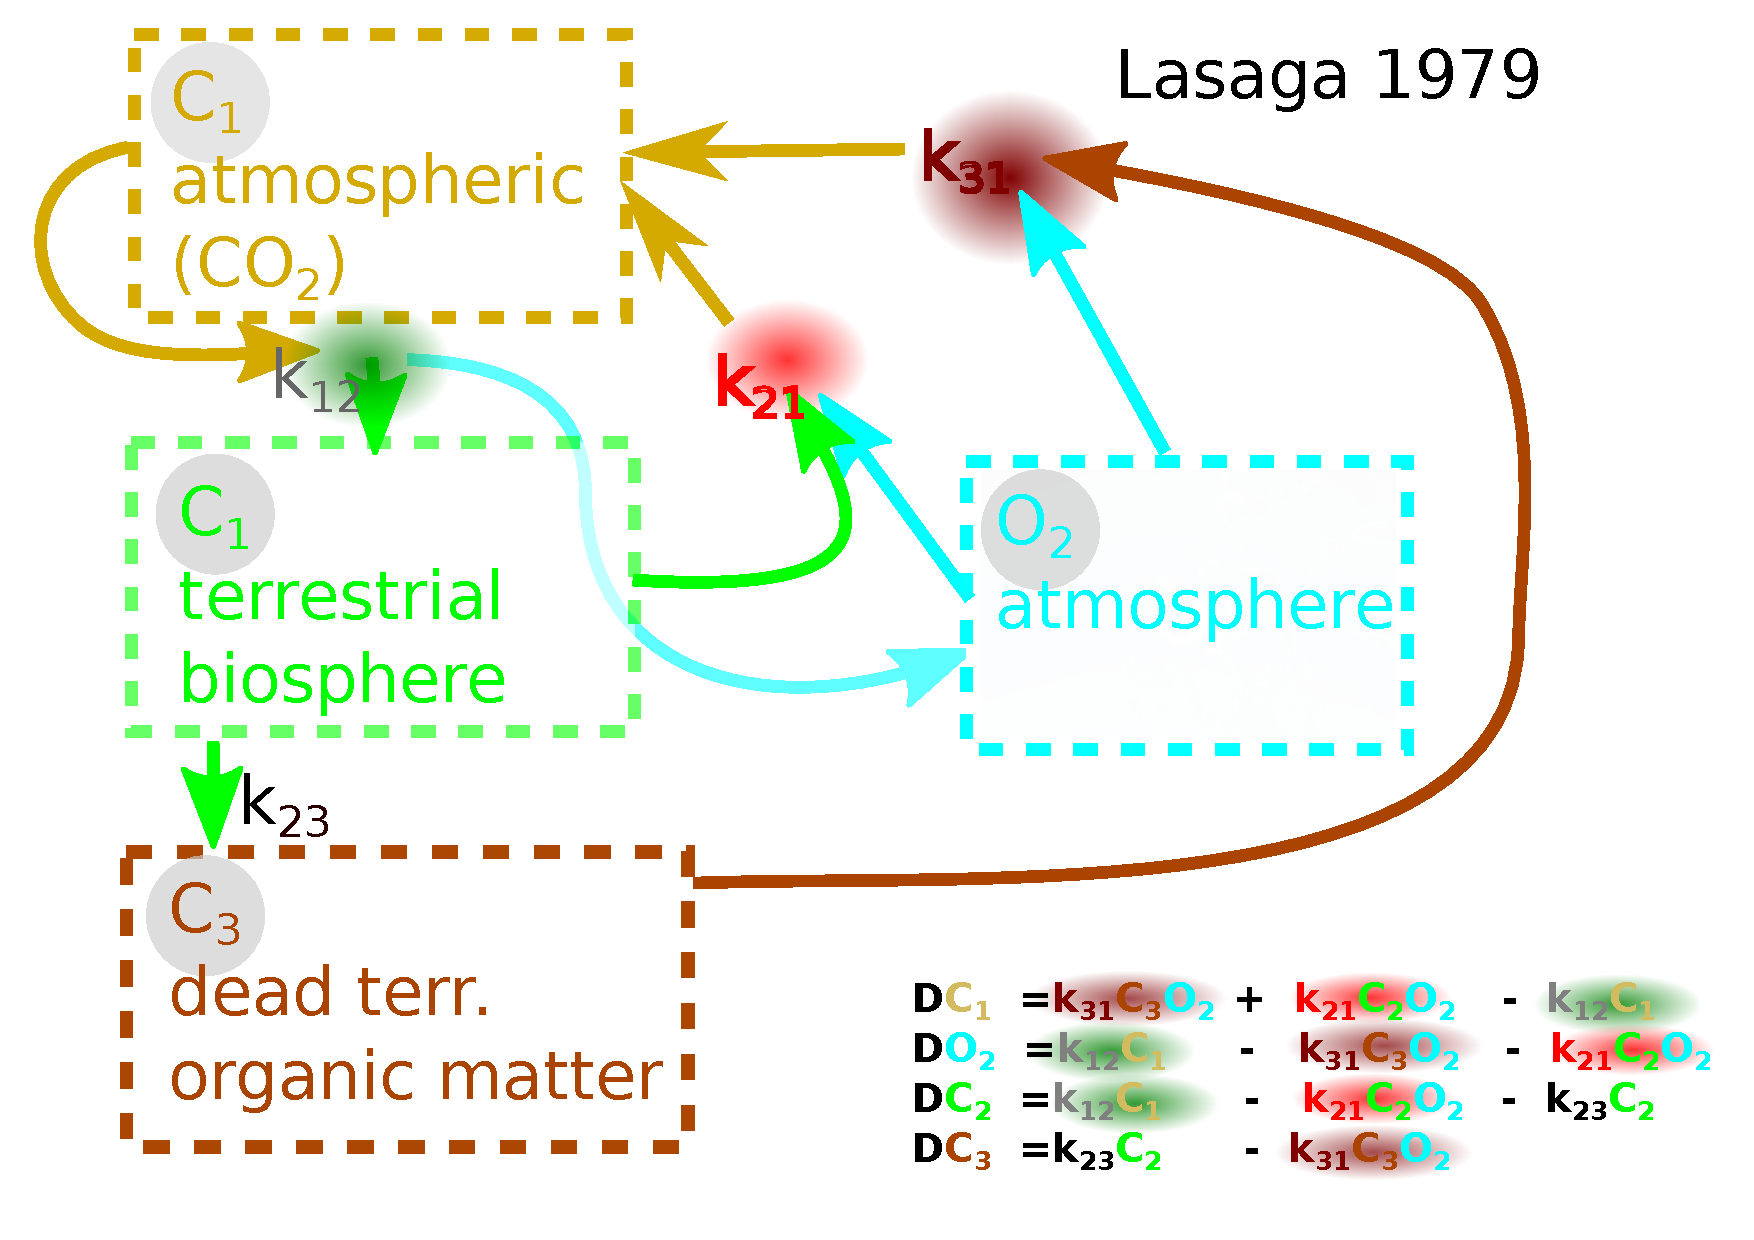
\includegraphics[width=0.9\textwidth]{LasagaModel.pdf}
\end{frame}
%%%%%%%%%%%%%%%%%%%%%%%%%%%%%%%%%%%%%%%%%%%%%%%%%%%%%%%%%%%%%%%%%%%%%%%%%%%%%%%%%%%%%%%%%%%%%%%%%%%%%
\begin{frame}
	\frametitle{Chemical Reactors}
	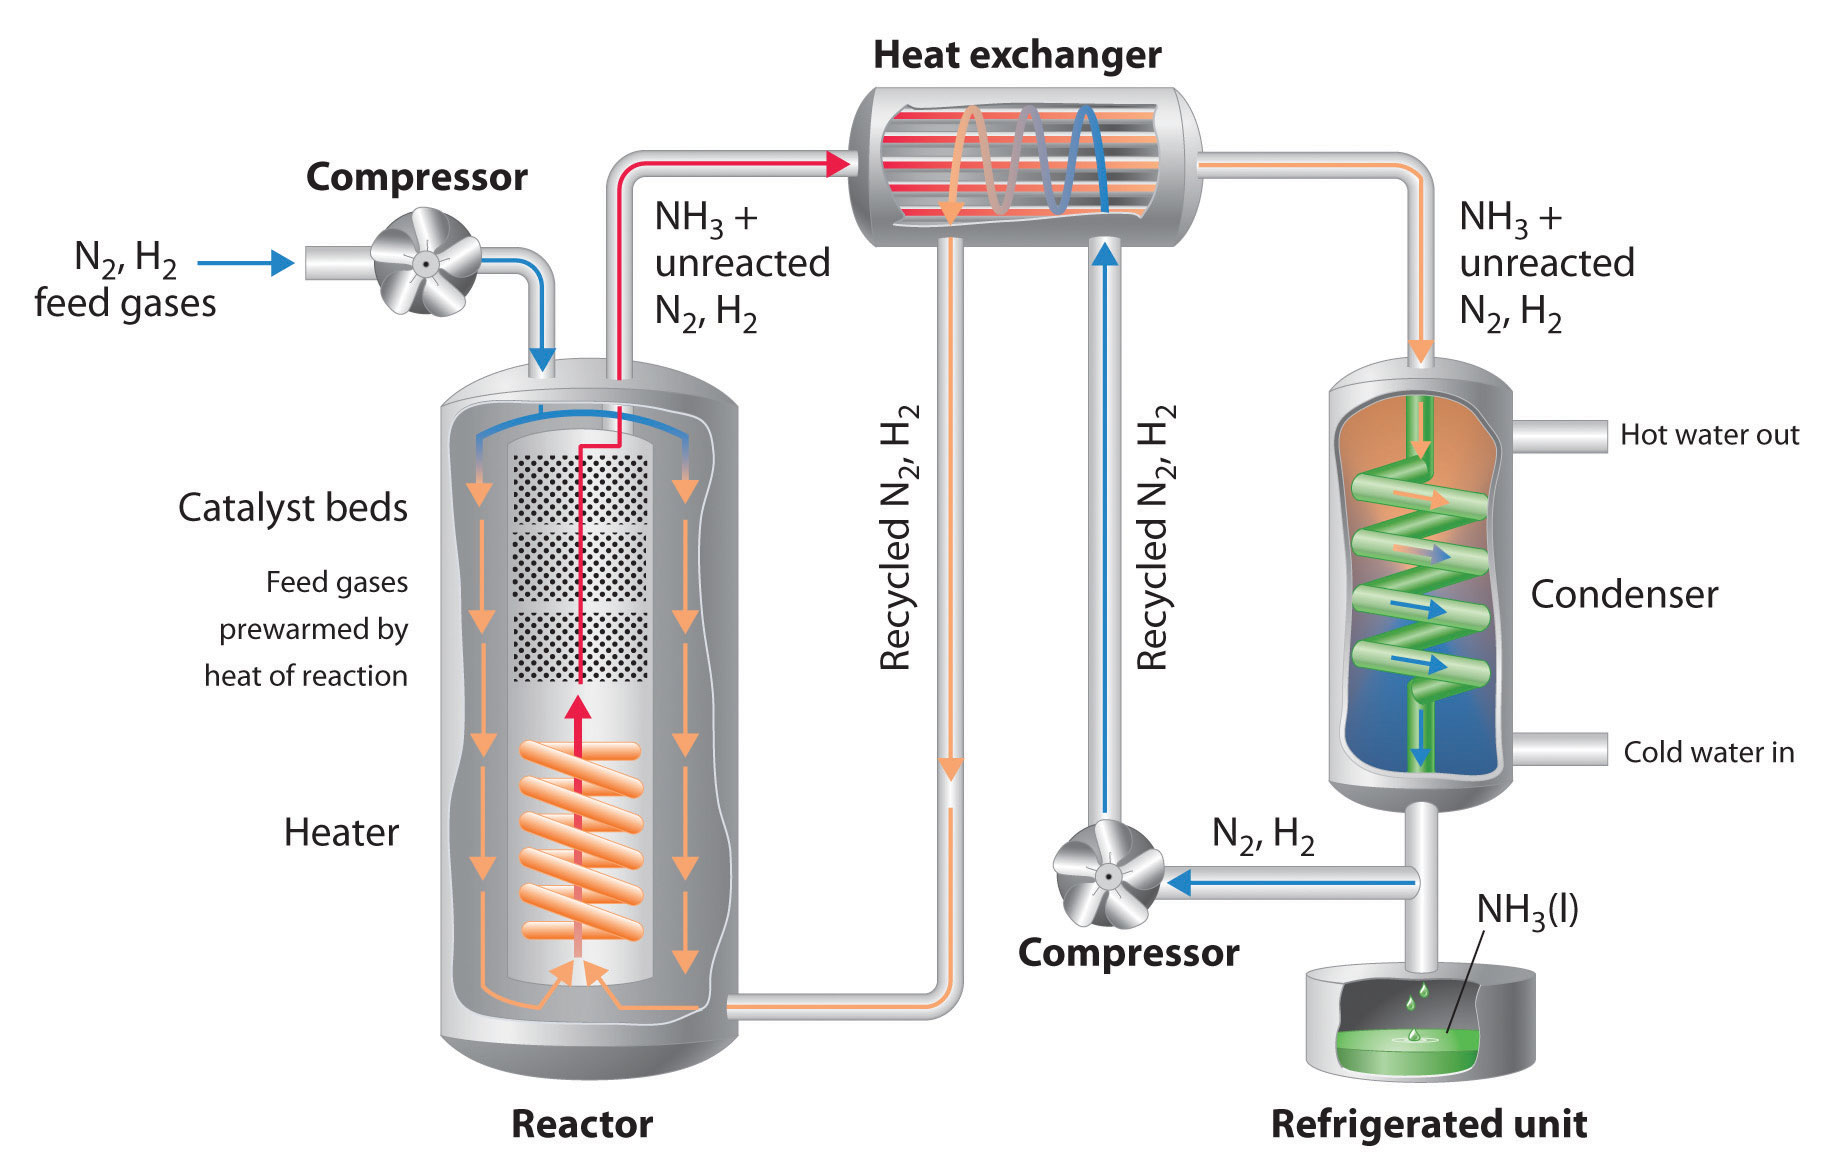
\includegraphics[width=0.9\textwidth]{HaberBosch.jpg}
\end{frame}
%%%%%%%%%%%%%%%%%%%%%%%%%%%%%%%%%%%%%%%%%%%%%%%%%%%%%%%%%%%%%%%%%%%%%%%%%%%%%%%%%%%%%%%%%%%%%%%%%%%%%
\begin{frame}
	\frametitle{Population Dynamics}
	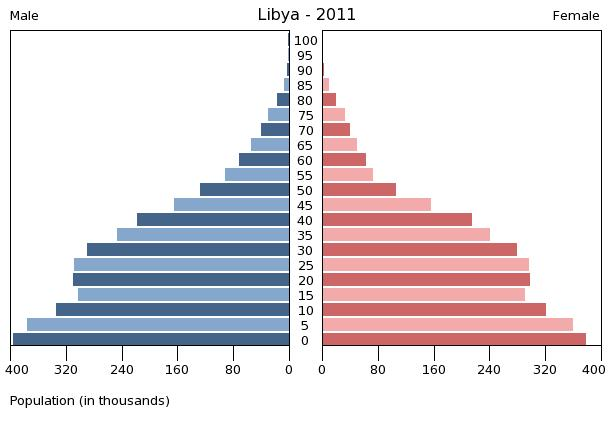
\includegraphics[width=0.9\textwidth]{LibyaPopulation2011.jpg}
\end{frame}
%%%%%%%%%%%%%%%%%%%%%%%%%%%%%%%%%%%%%%%%%%%%%%%%%%%%%%%%%%%%%%%%%%%%%%%%%%%%%%%%%%%%%%%%%%%%%%%%%%%%%
\section{Reducing Model Complexity }
\subsection{The Carbon Cycle example}
%%%%%%%%%%%%%%%%%%%%%%%%%%%%%%%%%%%%%%%%%%%%%%%%%%%%%%%%%%%%%%%%%%%%%%%%%%%%%%%%%%%%%%%%%%%%%%%%%%%%
%%%%%%%%%%%%%%%%%%%%%%%%%%%%%%%%%%%%%%%%%%%%%%%%%%%%%%%%%%%%%%%%%%%%%%%%%%%%%%%%%%%%%%%%%%%%%%%%%%%%%
\begin{frame}
  
\includegraphics[width=0.3\textwidth]{Earth.jpg}
\end{frame}
%%%%%%%%%%%%%%%%%%%%%%%%%%%%%%%%%%%%%%%%%%%%%%%%%%%%%%%%%%%%%%%%%%%%%%%%%%%%%%%%%%%%%%%%%%%%%%%%%%%%%
\begin{frame}
  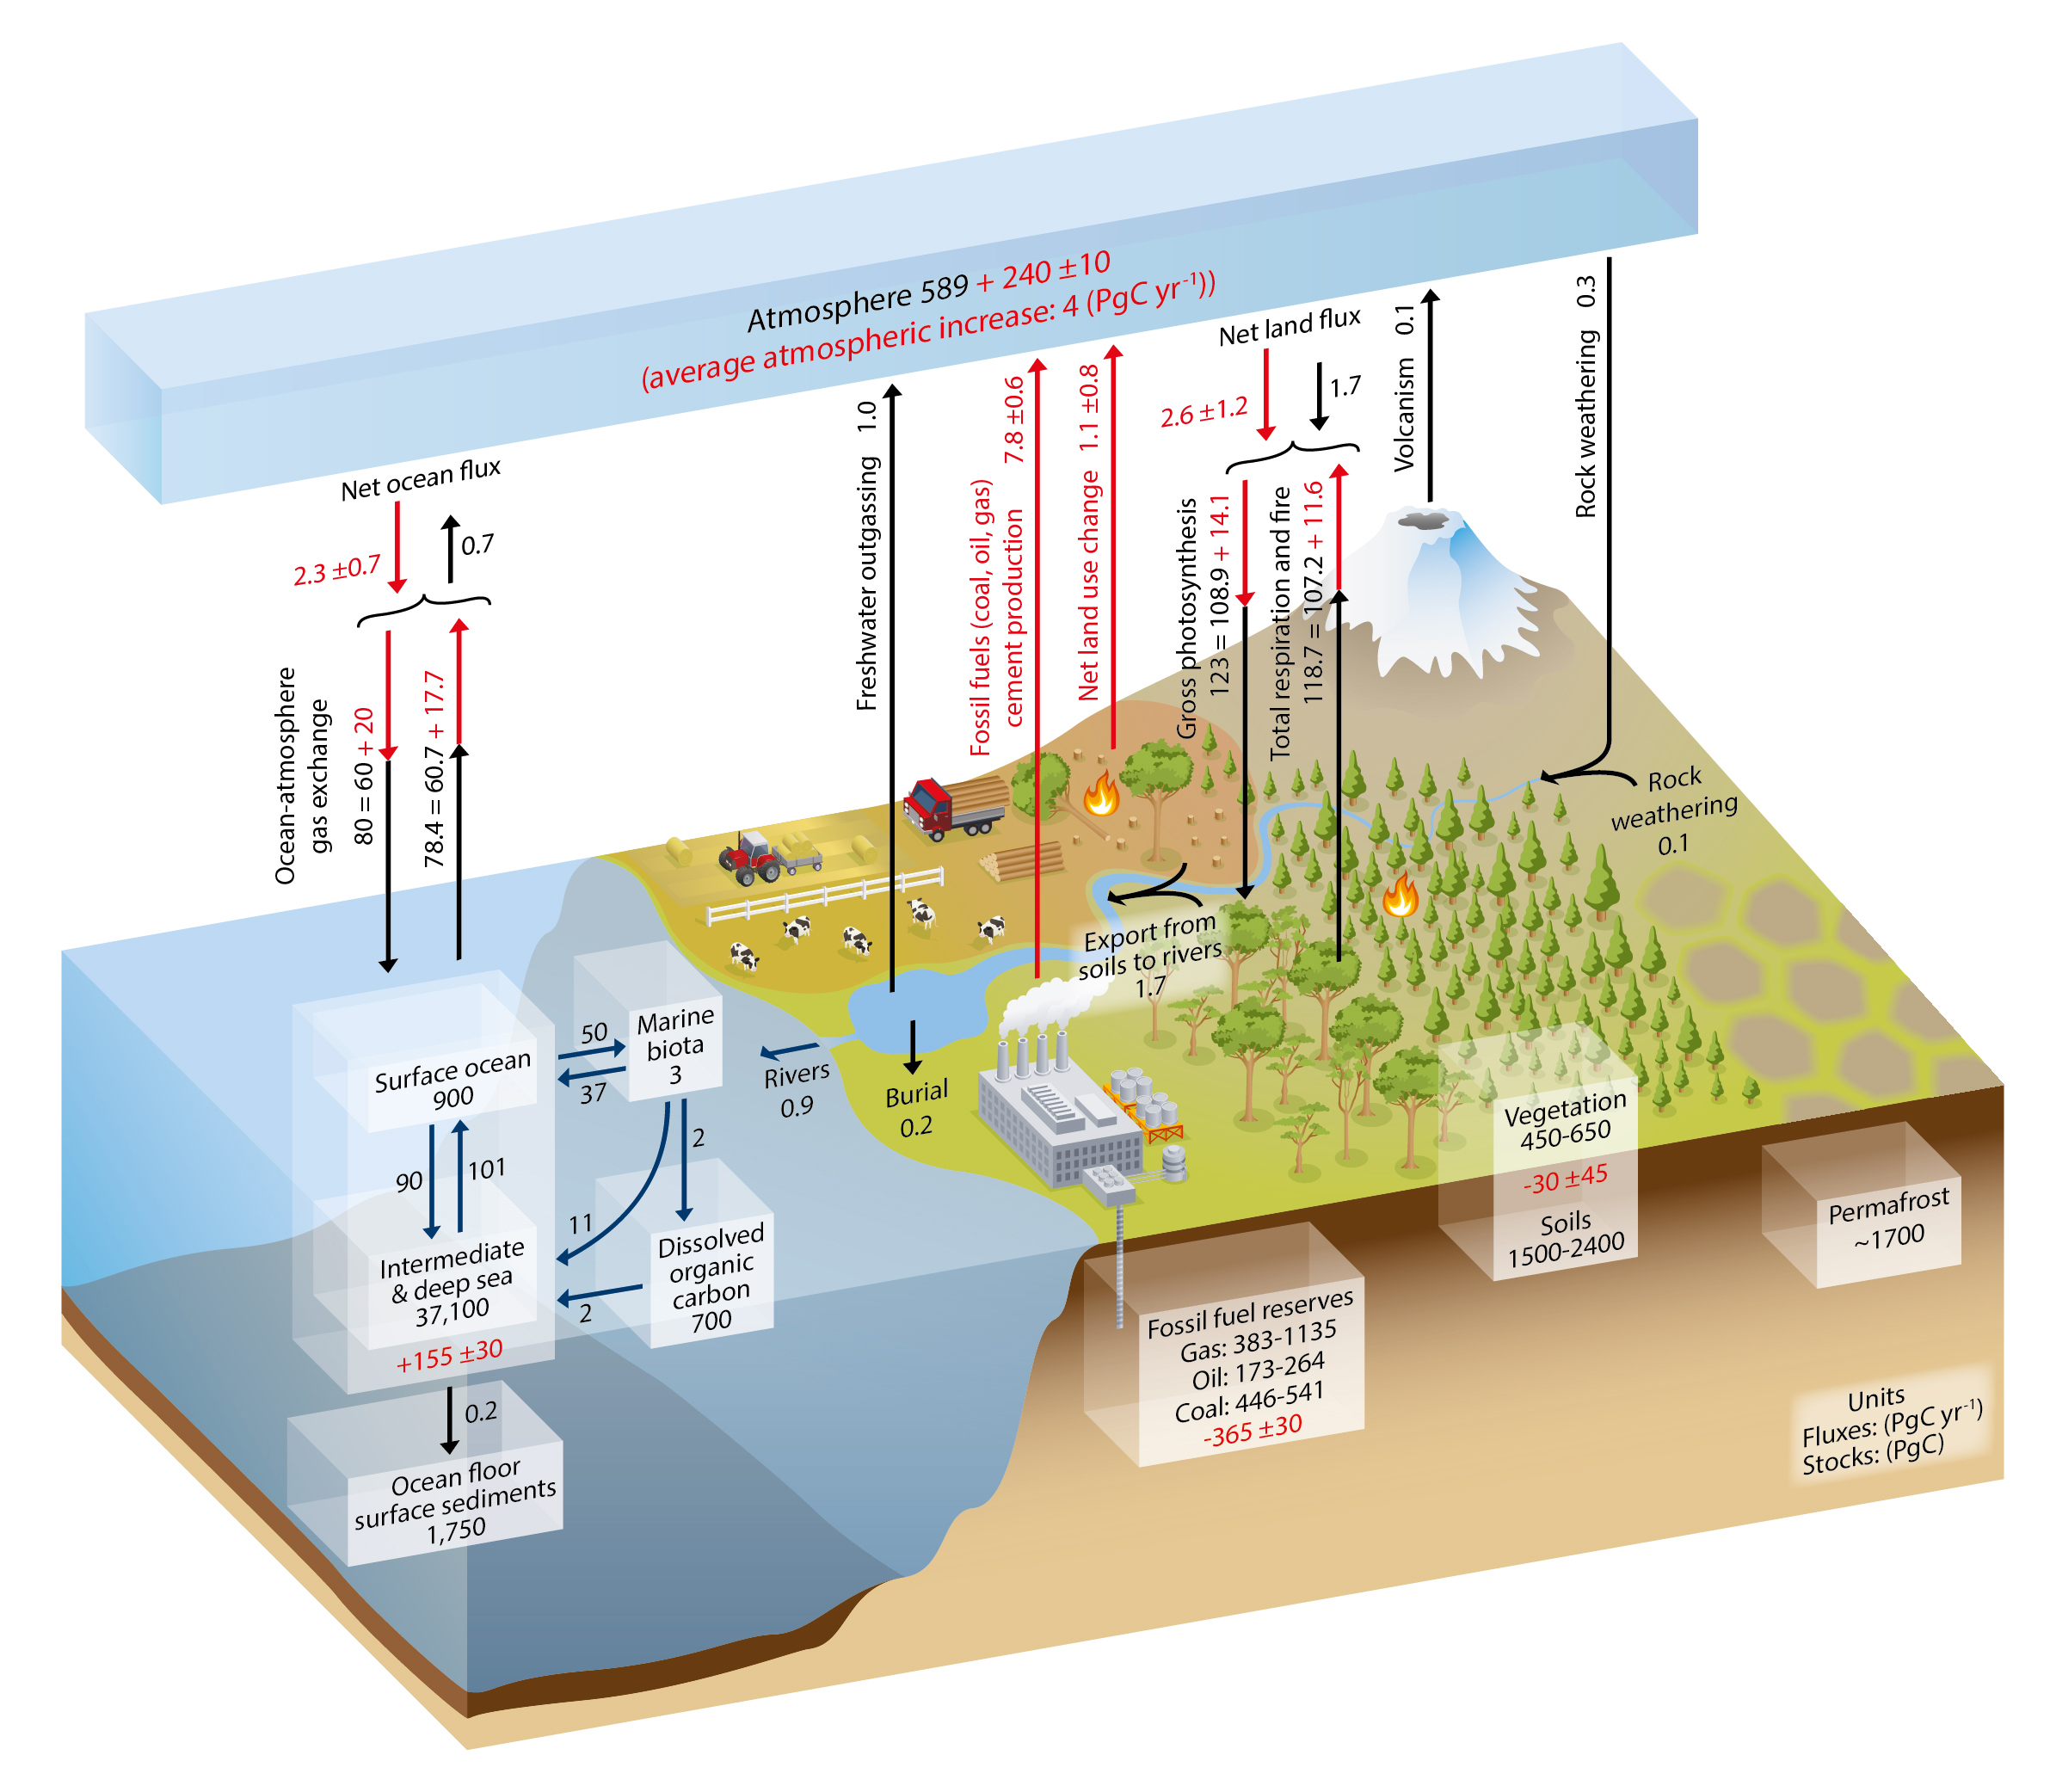
\includegraphics[width=0.9\textwidth]{cCycleIPCC.jpg}
\end{frame}
%%%%%%%%%%%%%%%%%%%%%%%%%%%%%%%%%%%%%%%%%%%%%%%%%%%%%%%%%%%%%%%%%%%%%%%%%%%%%%%%%%%%%%%%%%%%%%%%%%%%%
\begin{frame}
  
\includegraphics[width=0.3\textwidth]{Earth.jpg}
  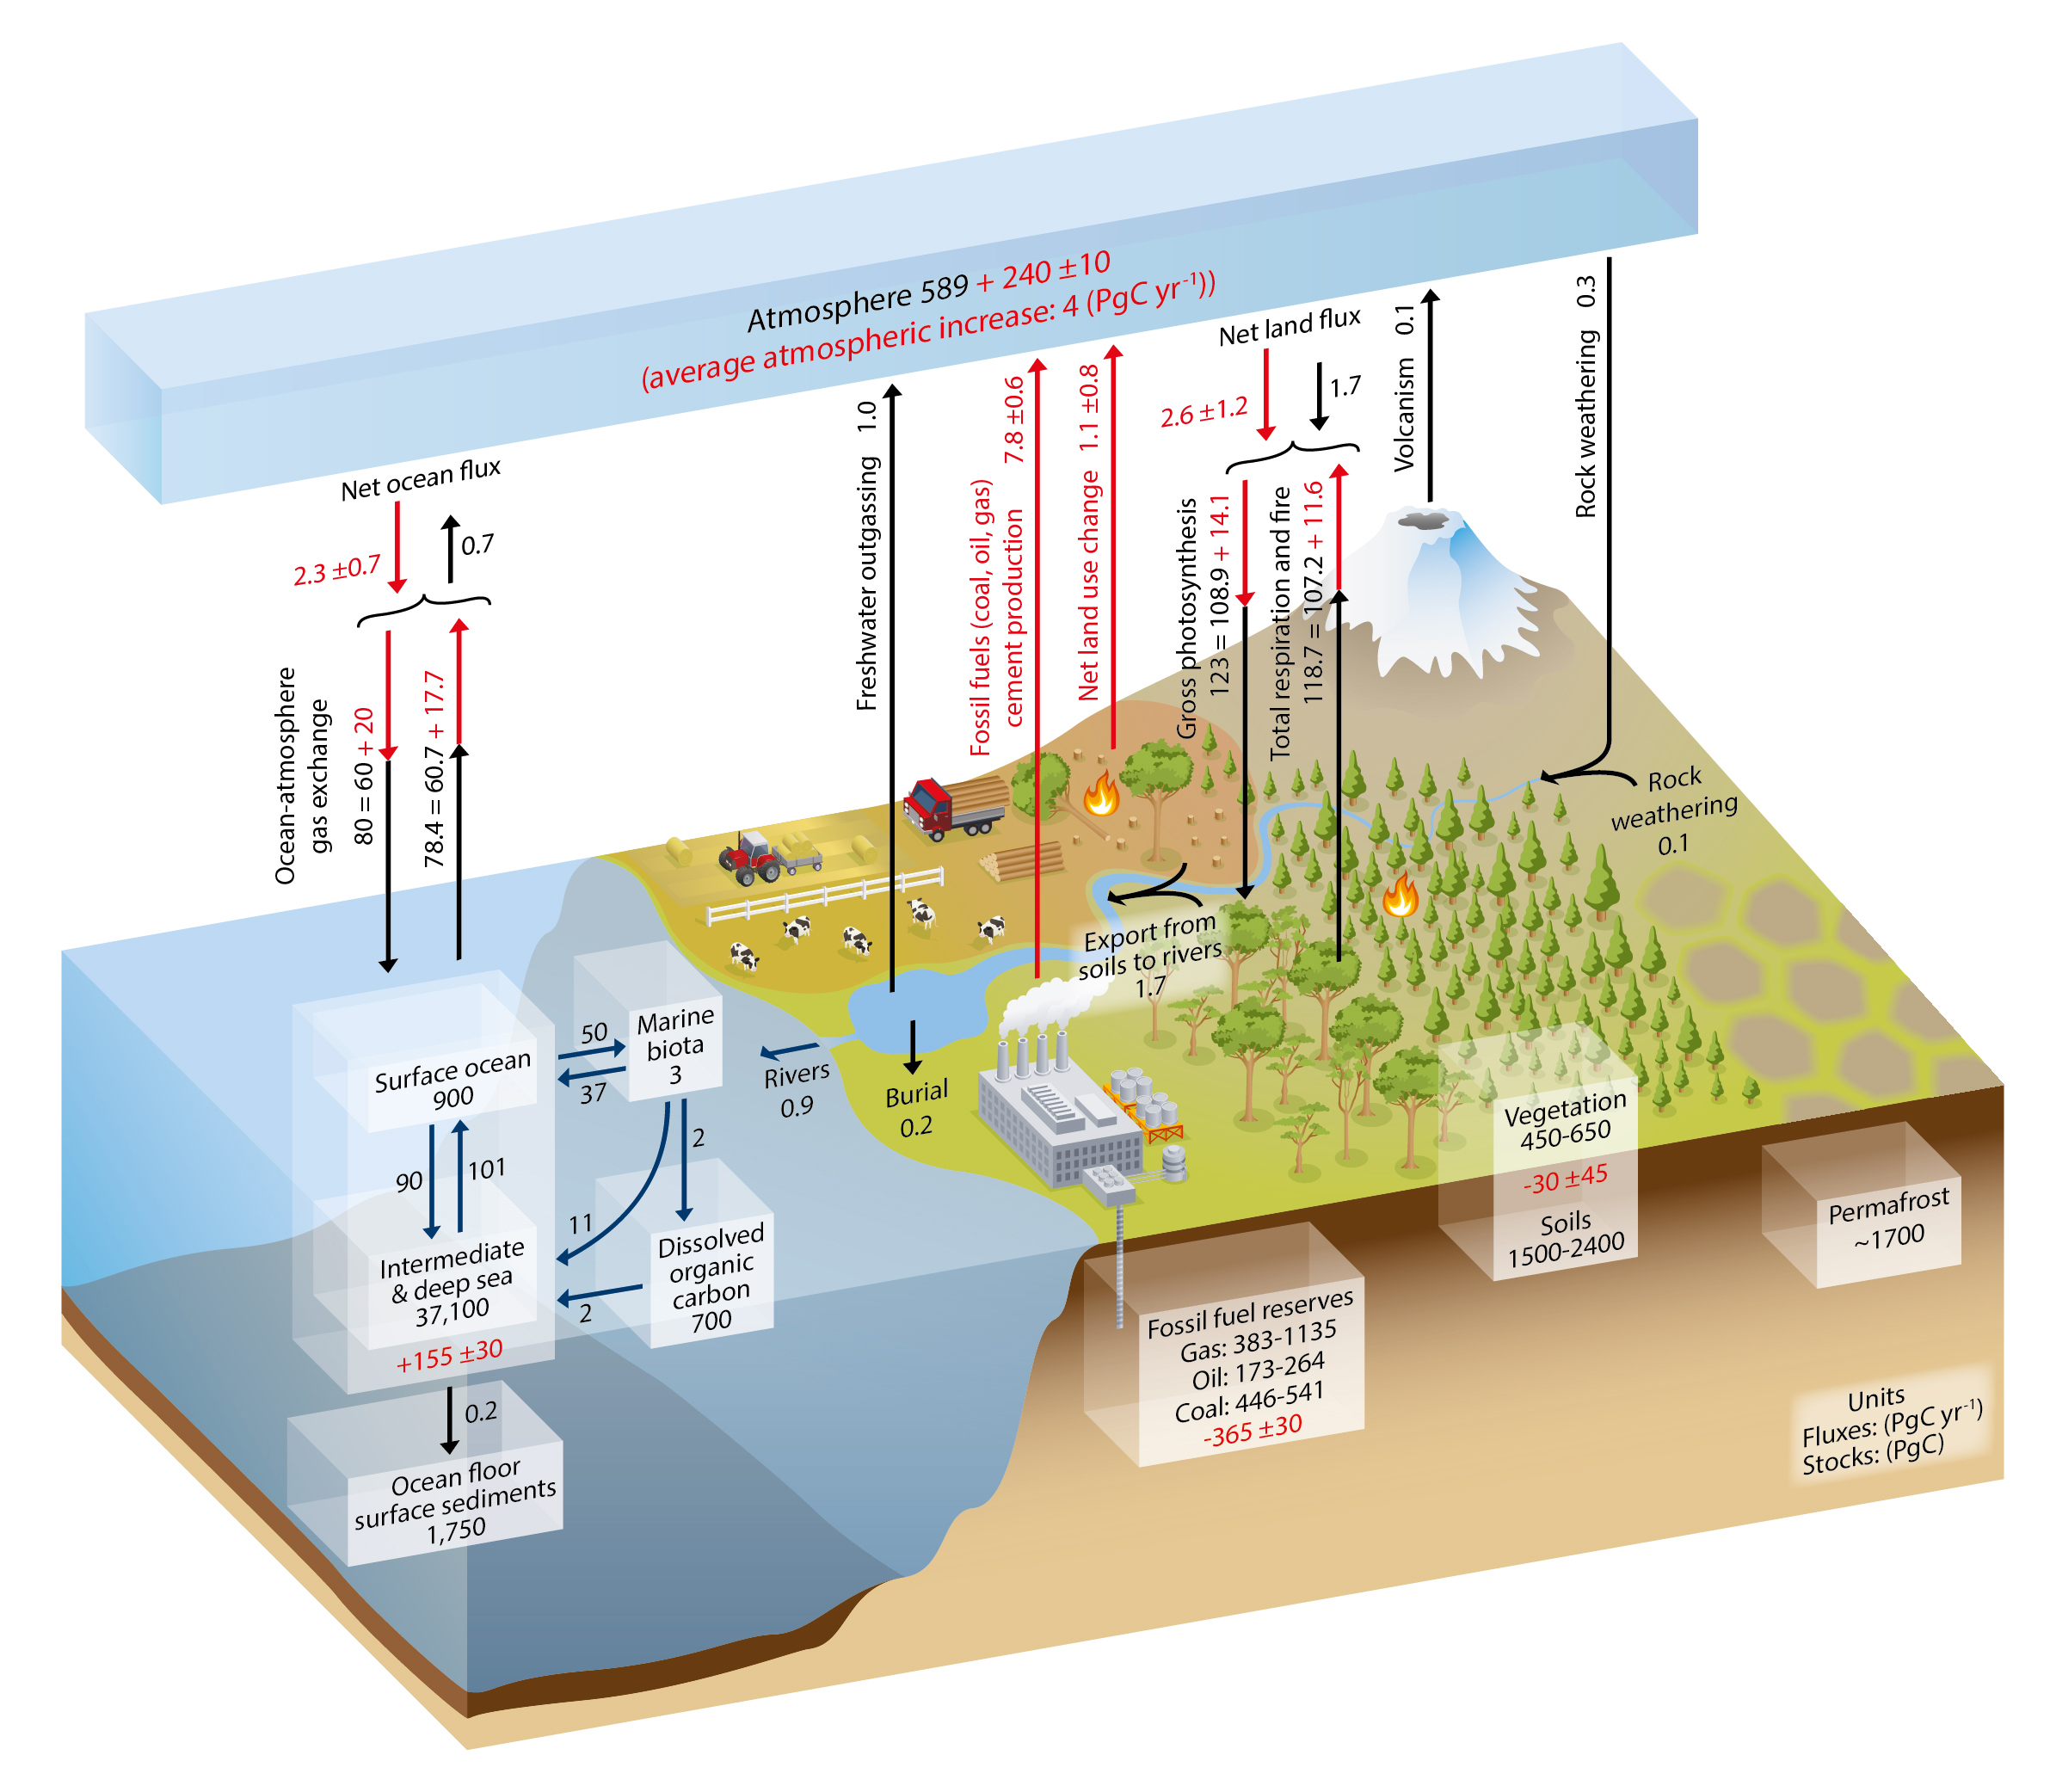
\includegraphics[width=0.3\textwidth]{cCycleIPCC.jpg}
  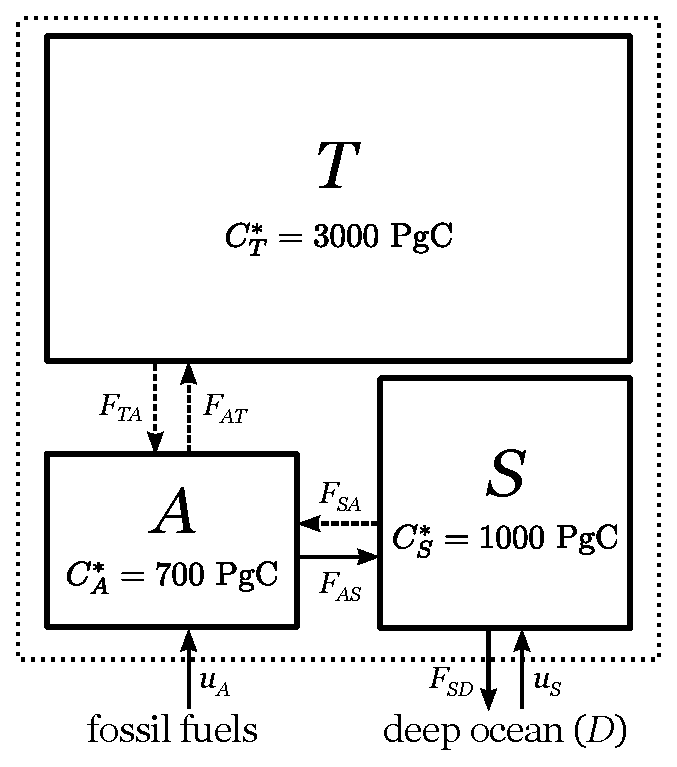
\includegraphics[width=0.35\textwidth]{model2.pdf}

\end{frame}
%%%%%%%%%%%%%%%%%%%%%%%%%%%%%%%%%%%%%%%%%%%%%%%%%%%%%%%%%%%%%%%%%%%%%%%%%%%%%%%%%%%%%%%%%%%%%%%%%%%%%
\subsection{Asking Simpler Questions}
%%%%%%%%%%%%%%%%%%%%%%%%%%%%%%%%%%%%%%%%%%%%%%%%%%%%%%%%%%%%%%%%%%%%%%%%%%%%%%%%%%%%%%%%%%%%%%%%%%%%%
\begin{frame}
	\frametitle{}
	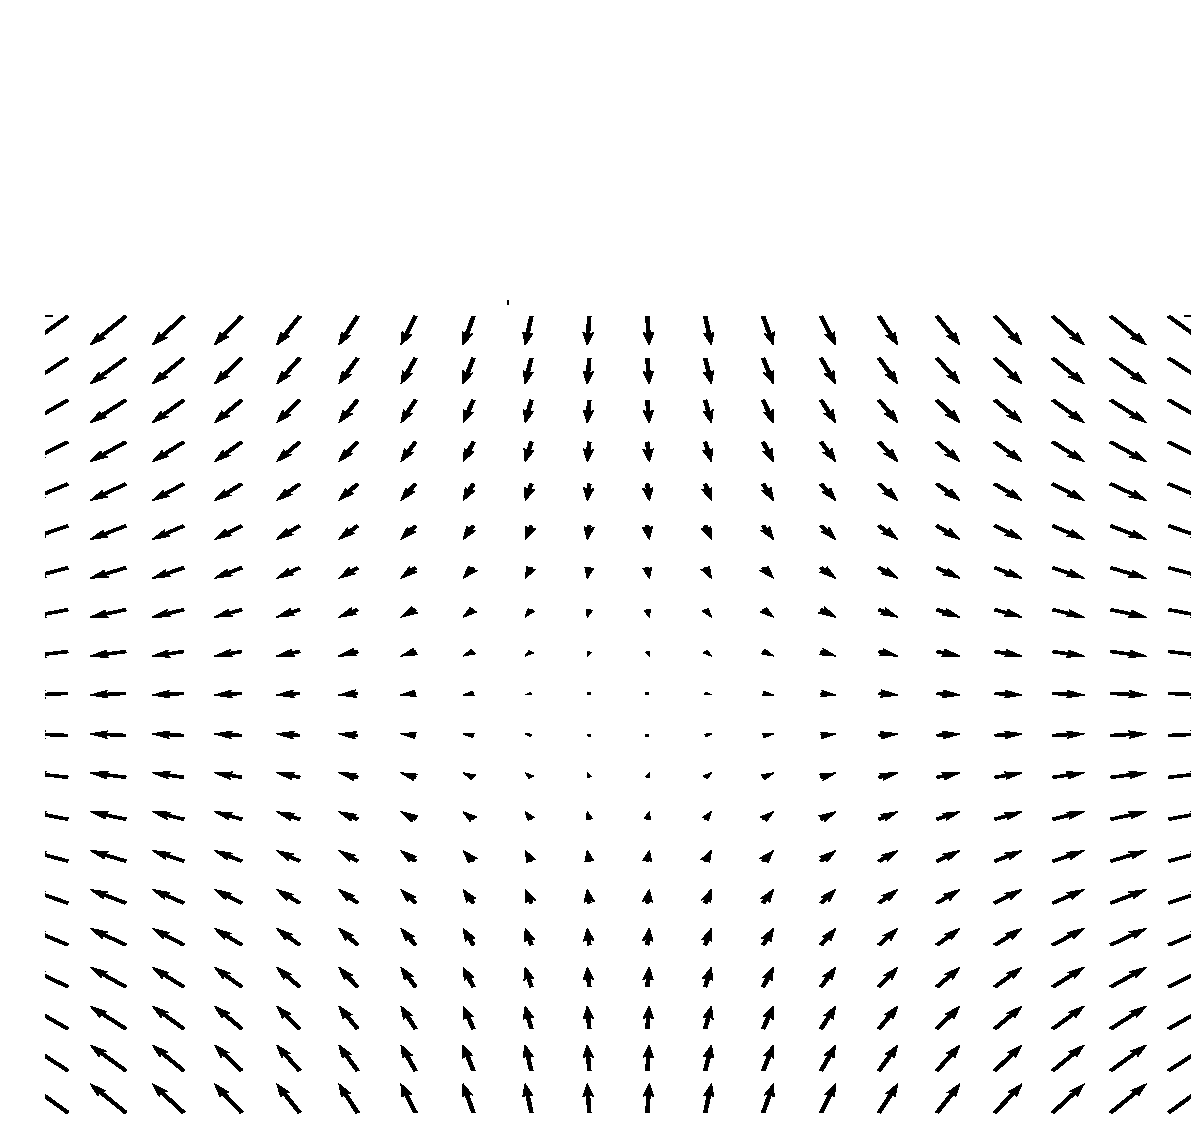
\includegraphics[width=0.9\textwidth]{Solenoidal_vector_field_2.pdf}
\end{frame}
%%%%%%%%%%%%%%%%%%%%%%%%%%%%%%%%%%%%%%%%%%%%%%%%%%%%%%%%%%%%%%%%%%%%%%%%%%%%%%%%%%%%%%%%%%%%%%%%%%%%%
\begin{frame}
	\frametitle{}
	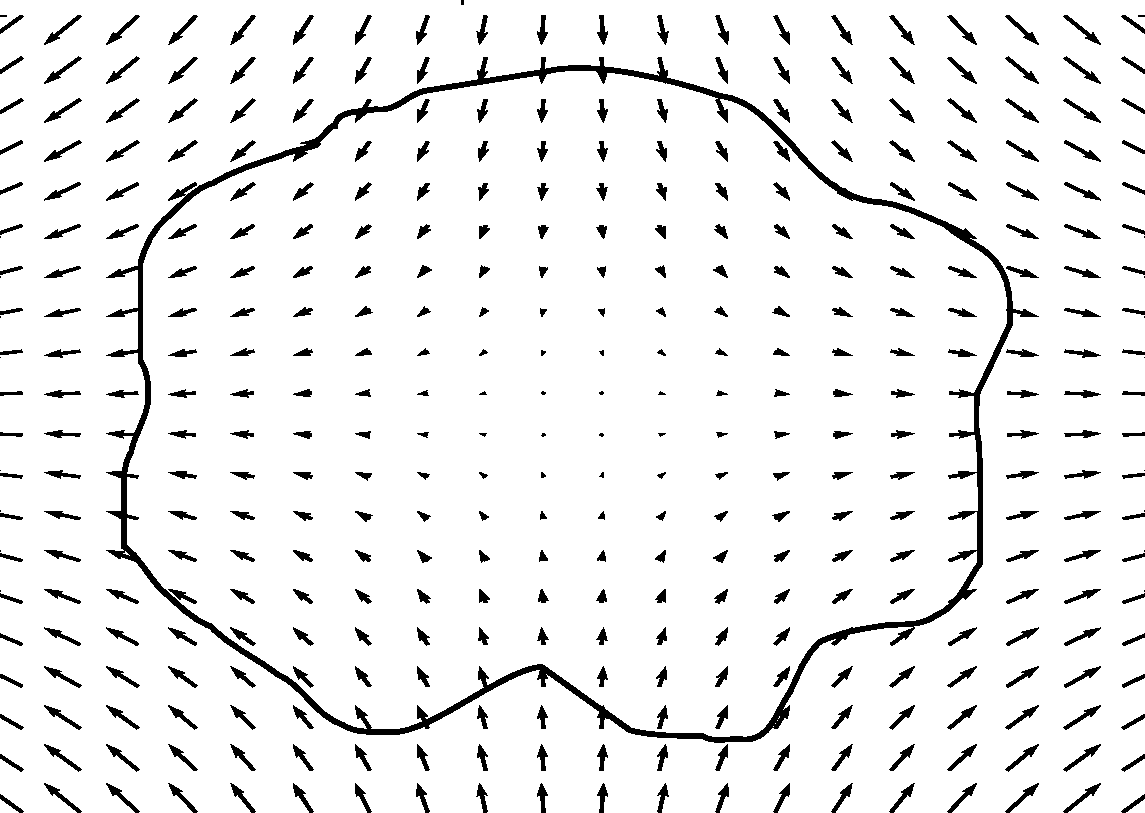
\includegraphics[width=0.9\textwidth]{VectorFieldWithOnePool.pdf}
\end{frame}
%%%%%%%%%%%%%%%%%%%%%%%%%%%%%%%%%%%%%%%%%%%%%%%%%%%%%%%%%%%%%%%%%%%%%%%%%%%%%%%%%%%%%%%%%%%%%%%%%%%%%
\begin{frame}
	\frametitle{}
	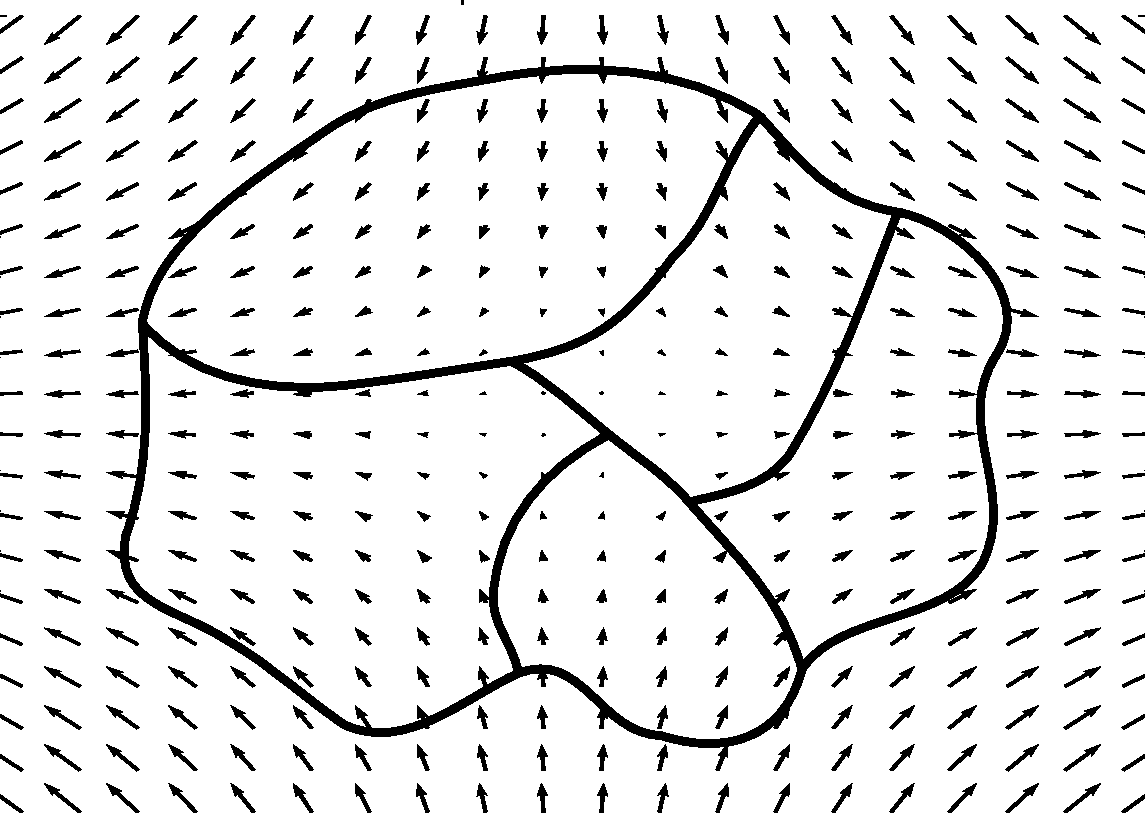
\includegraphics[width=0.9\textwidth]{VectorFieldWithOnePoolAndSubpools.pdf}
\end{frame}
%%%%%%%%%%%%%%%%%%%%%%%%%%%%%%%%%%%%%%%%%%%%%%%%%%%%%%%%%%%%%%%%%%%%%%%%%%%%%%%%%%%%%%%%%%%%%%%%%%%%%
\begin{frame}
	\frametitle{}
	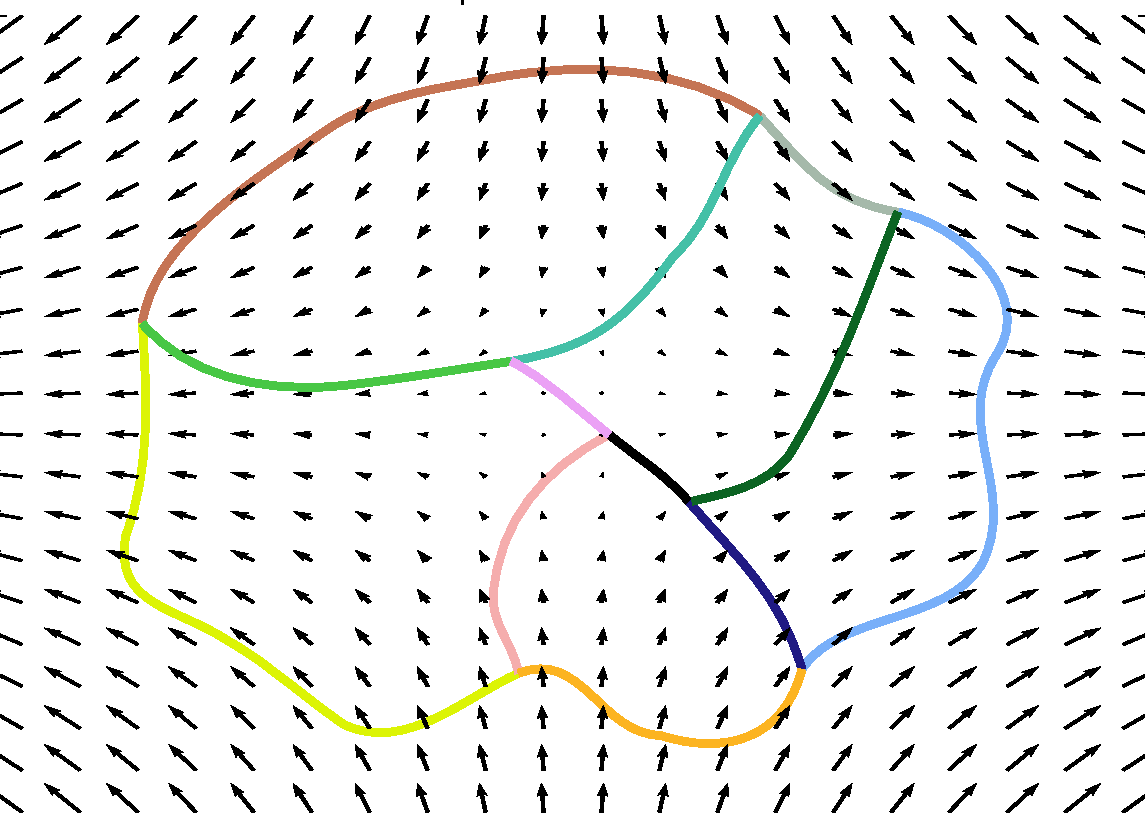
\includegraphics[width=0.9\textwidth]{VectorFieldWithOnePoolAndSubpoolsAndColoredBoundaries.pdf}
\end{frame}
%%%%%%%%%%%%%%%%%%%%%%%%%%%%%%%%%%%%%%%%%%%%%%%%%%%%%%%%%%%%%%%%%%%%%%%%%%%%%%%%%%%%%%%%%%%%%%%%%%%%%
\begin{frame}
	\frametitle{}
	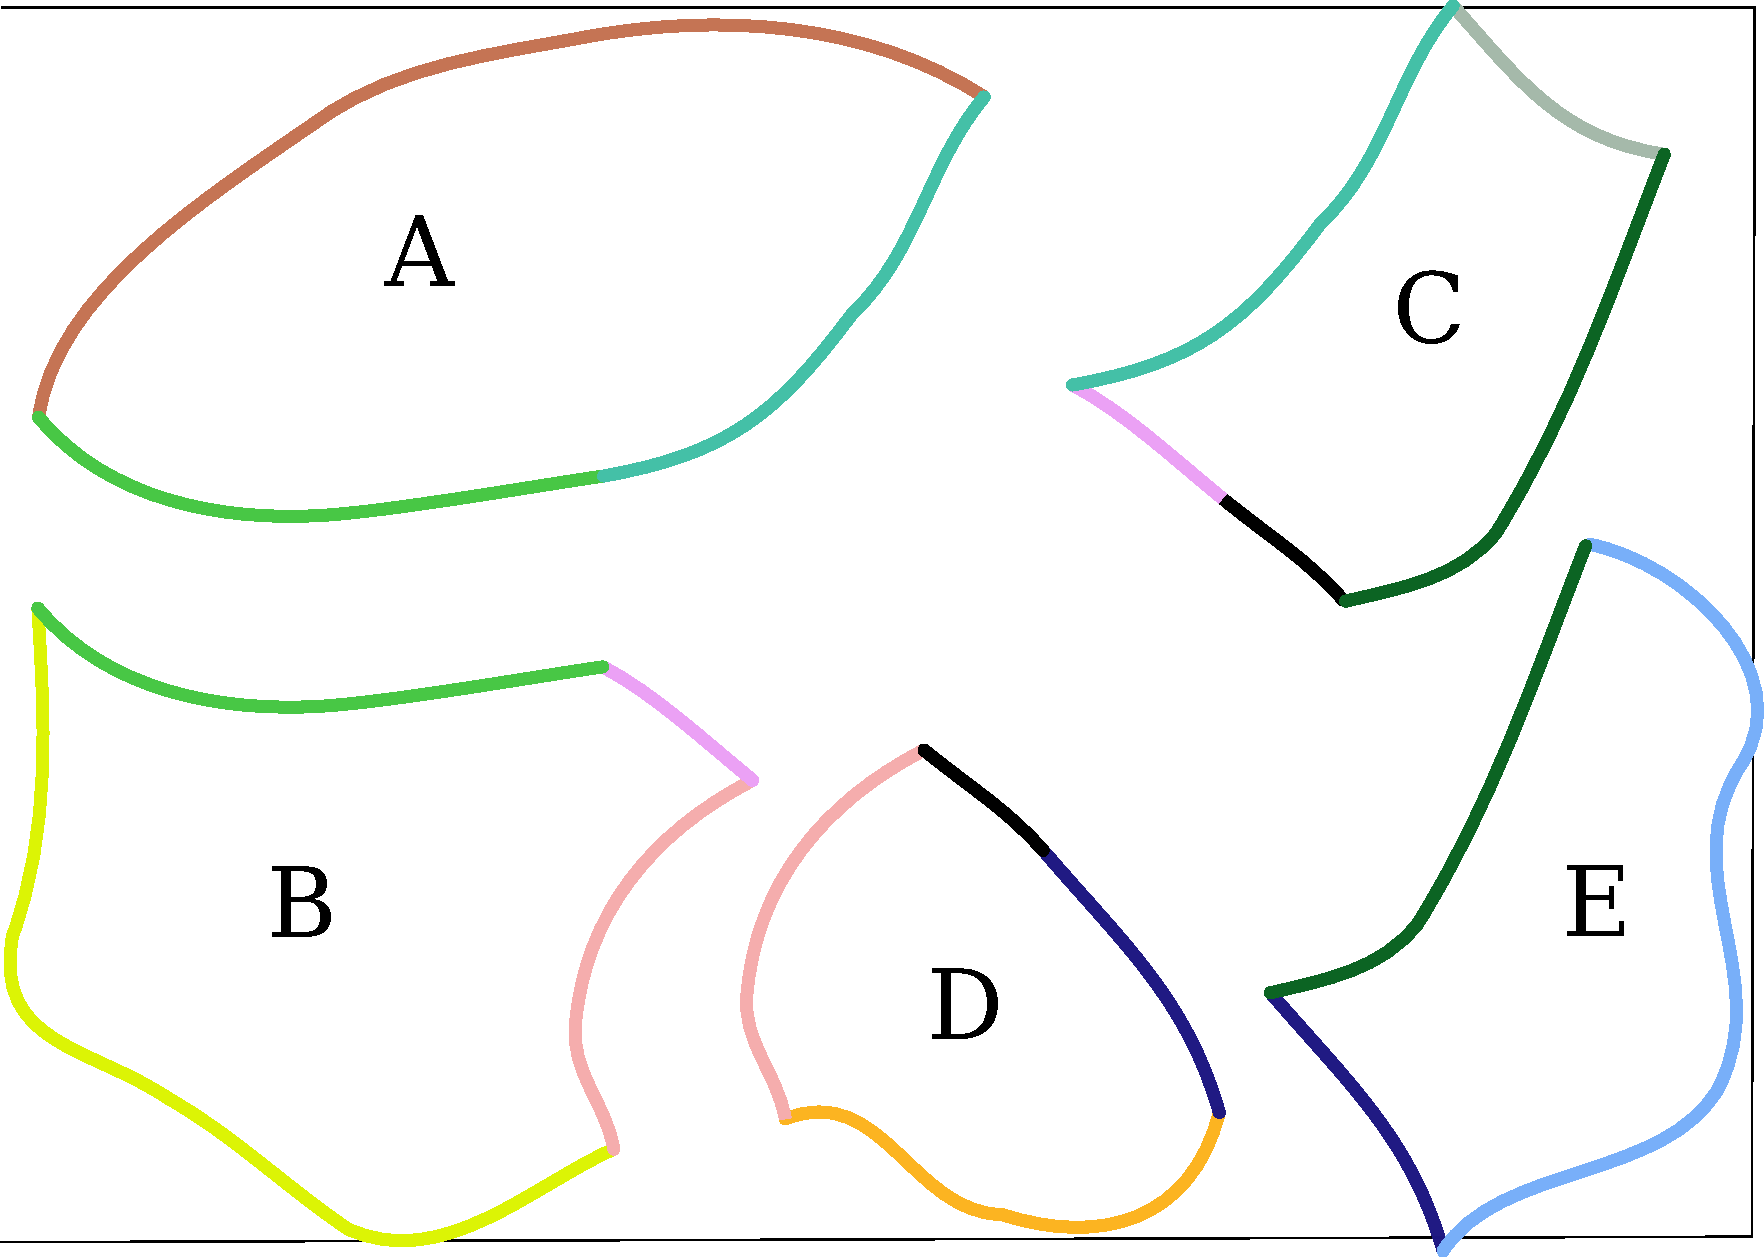
\includegraphics[width=0.9\textwidth]{SubpoolsAndColoredBoundaries.pdf}
\end{frame}
%%%%%%%%%%%%%%%%%%%%%%%%%%%%%%%%%%%%%%%%%%%%%%%%%%%%%%%%%%%%%%%%%%%%%%%%%%%%%%%%%%%%%%%%%%%%%%%%%%%%%
\begin{frame}
	\frametitle{}
	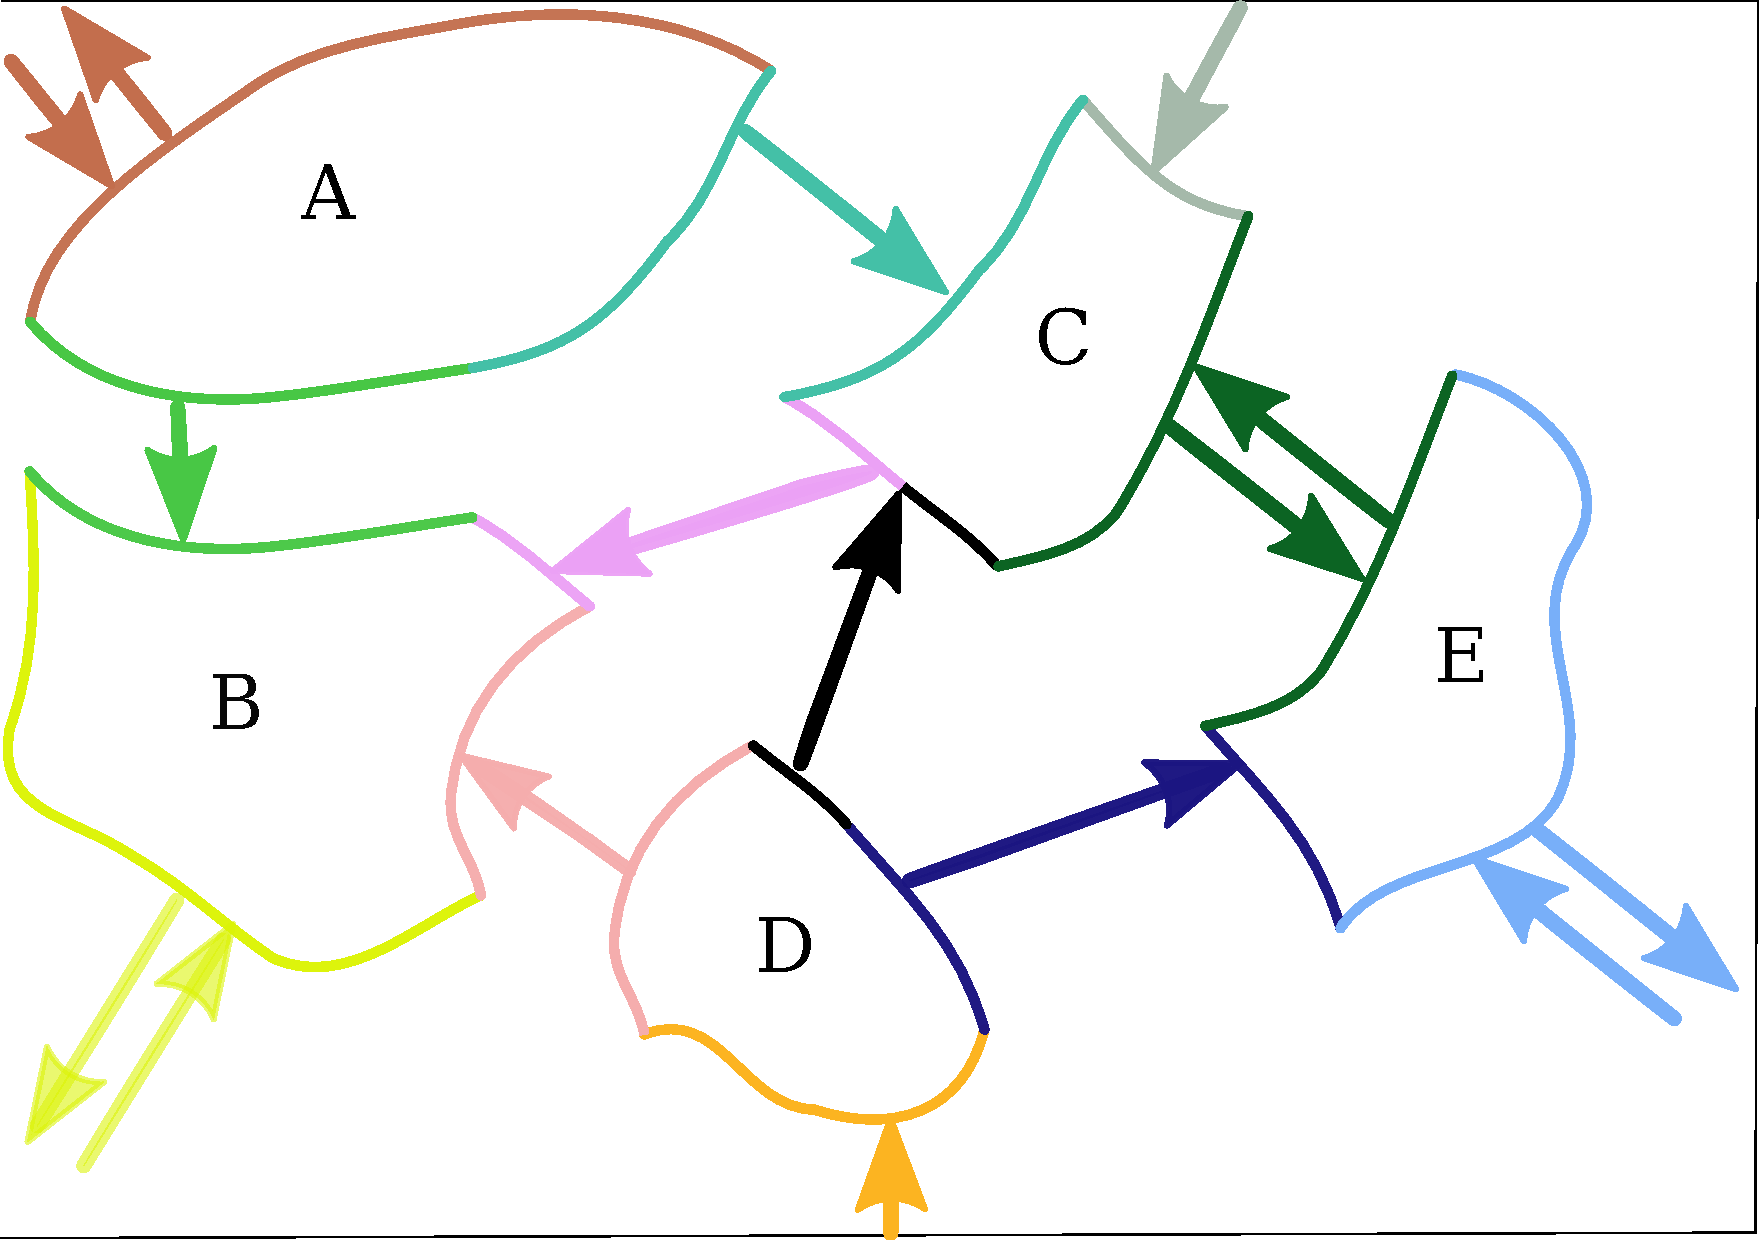
\includegraphics[width=0.9\textwidth]{SubpoolsAndColoredBoundariesAndArrows.pdf}
\end{frame}
%%%%%%%%%%%%%%%%%%%%%%%%%%%%%%%%%%%%%%%%%%%%%%%%%%%%%%%%%%%%%%%%%%%%%%%%%%%%%%%%%%%%%%%%%%%%%%%%%%%%%
\begin{frame}
	\frametitle{}
	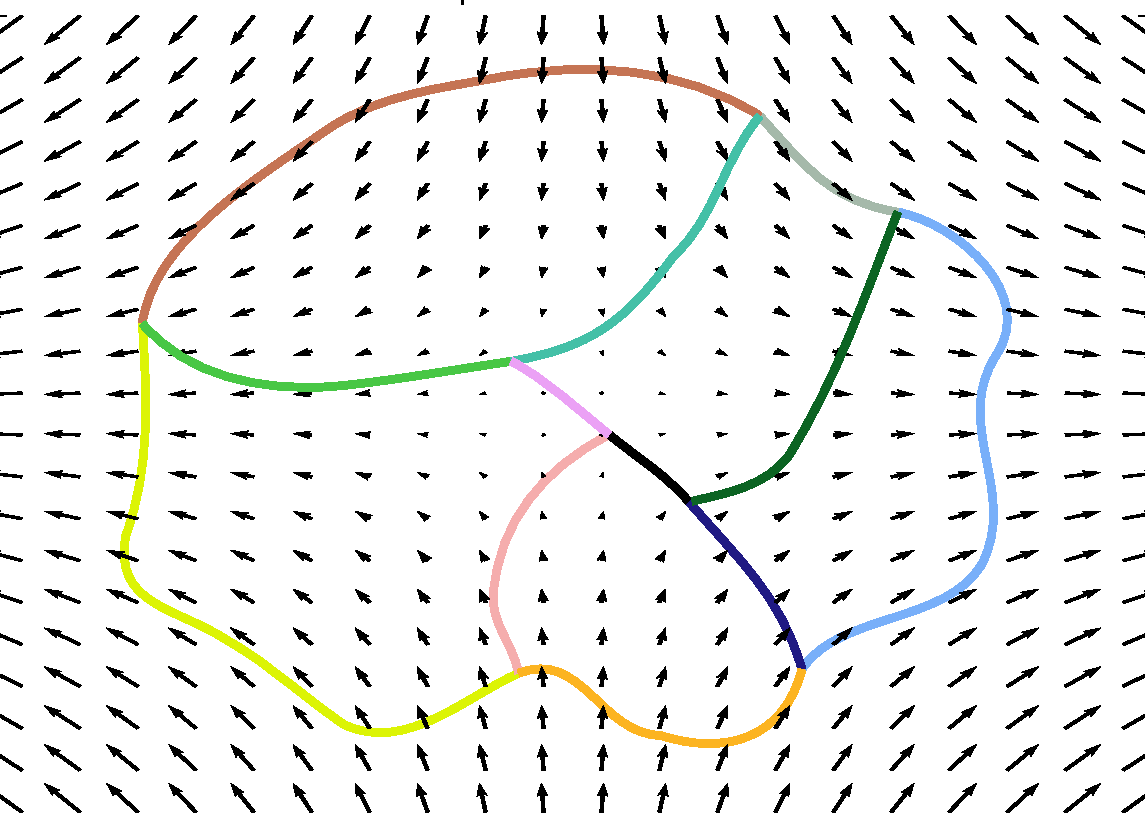
\includegraphics[width=0.45\textwidth]{VectorFieldWithOnePoolAndSubpoolsAndColoredBoundaries.pdf}
	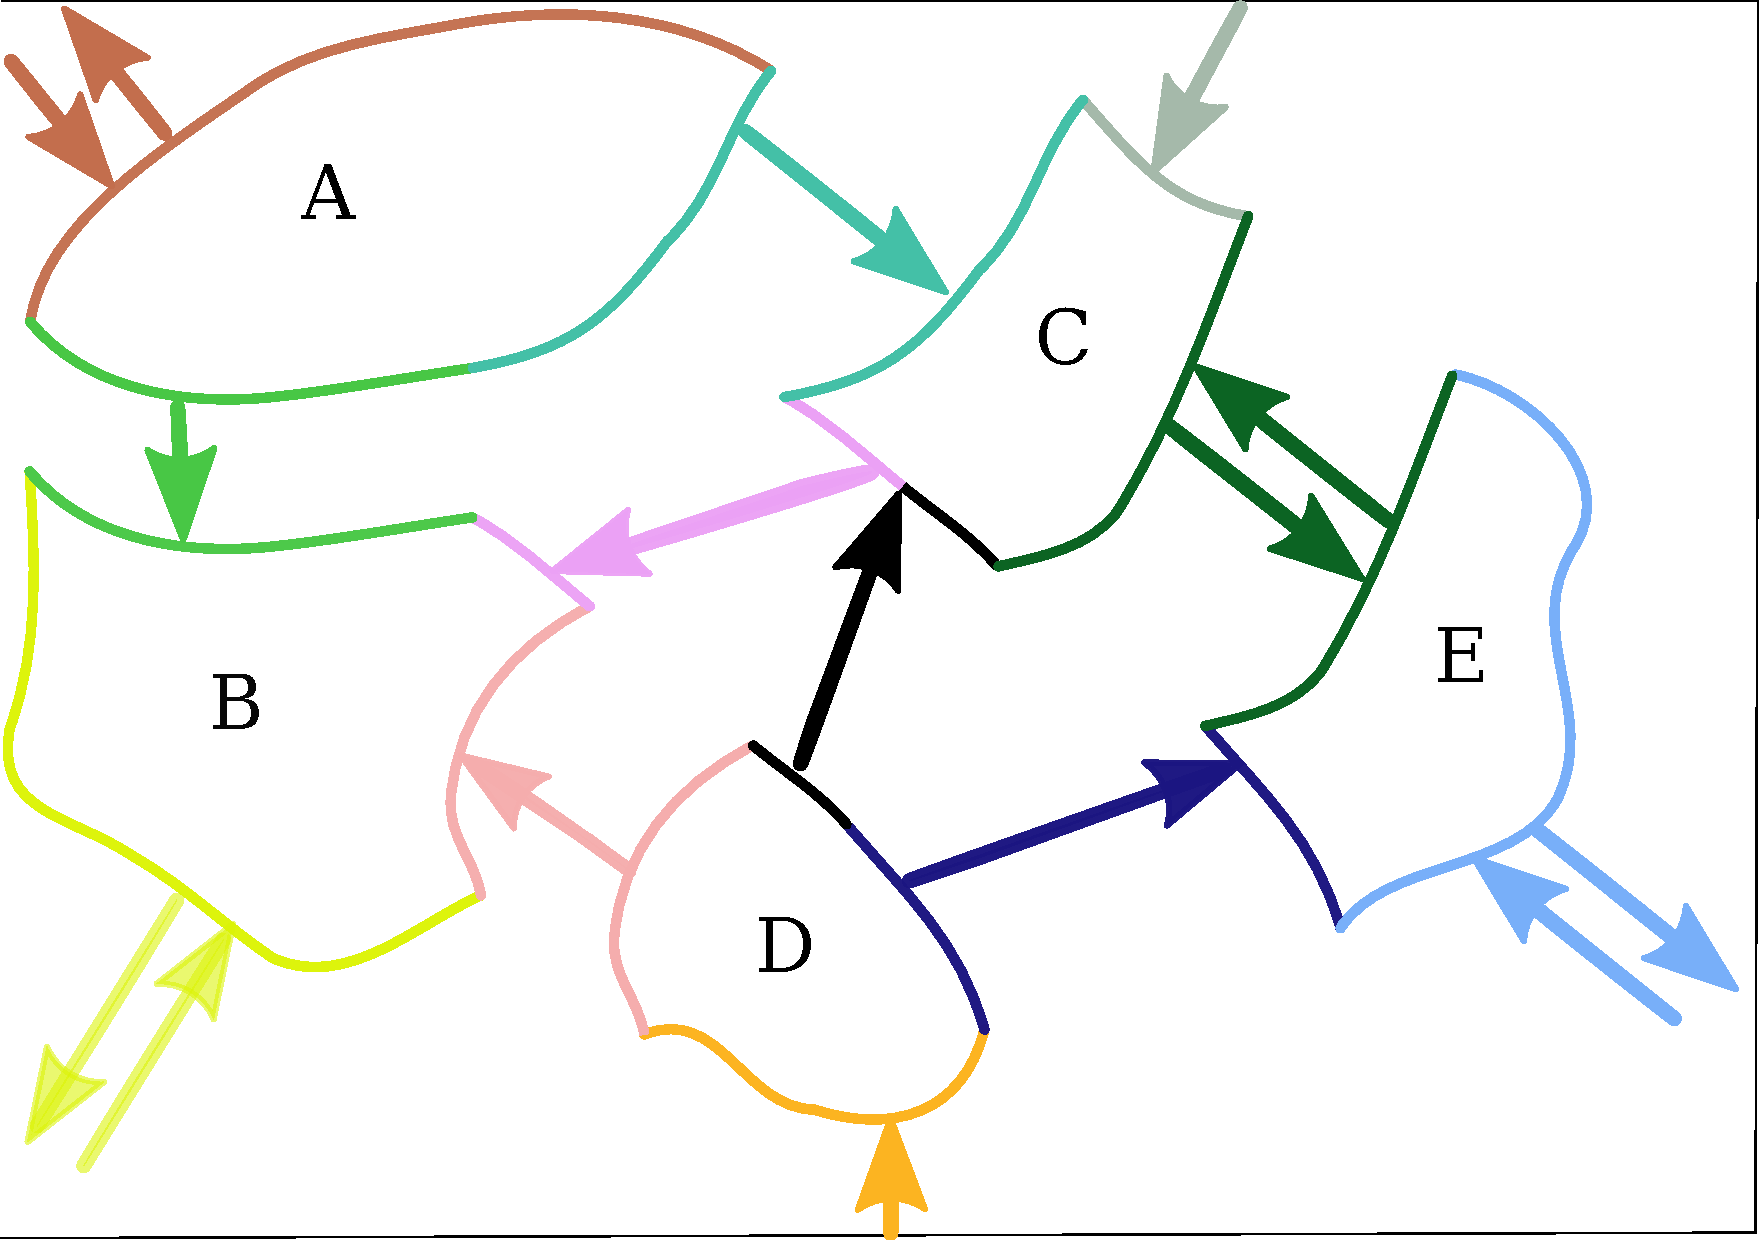
\includegraphics[width=0.45\textwidth]{SubpoolsAndColoredBoundariesAndArrows.pdf}
\end{frame}
%%%%%%%%%%%%%%%%%%%%%%%%%%%%%%%%%%%%%%%%%%%%%%%%%%%%%%%%%%%%%%%%%%%%%%%%%%%%%%%%%%%%%%%%%%%%%%%%%%%%%
\begin{frame}
	\frametitle{}
	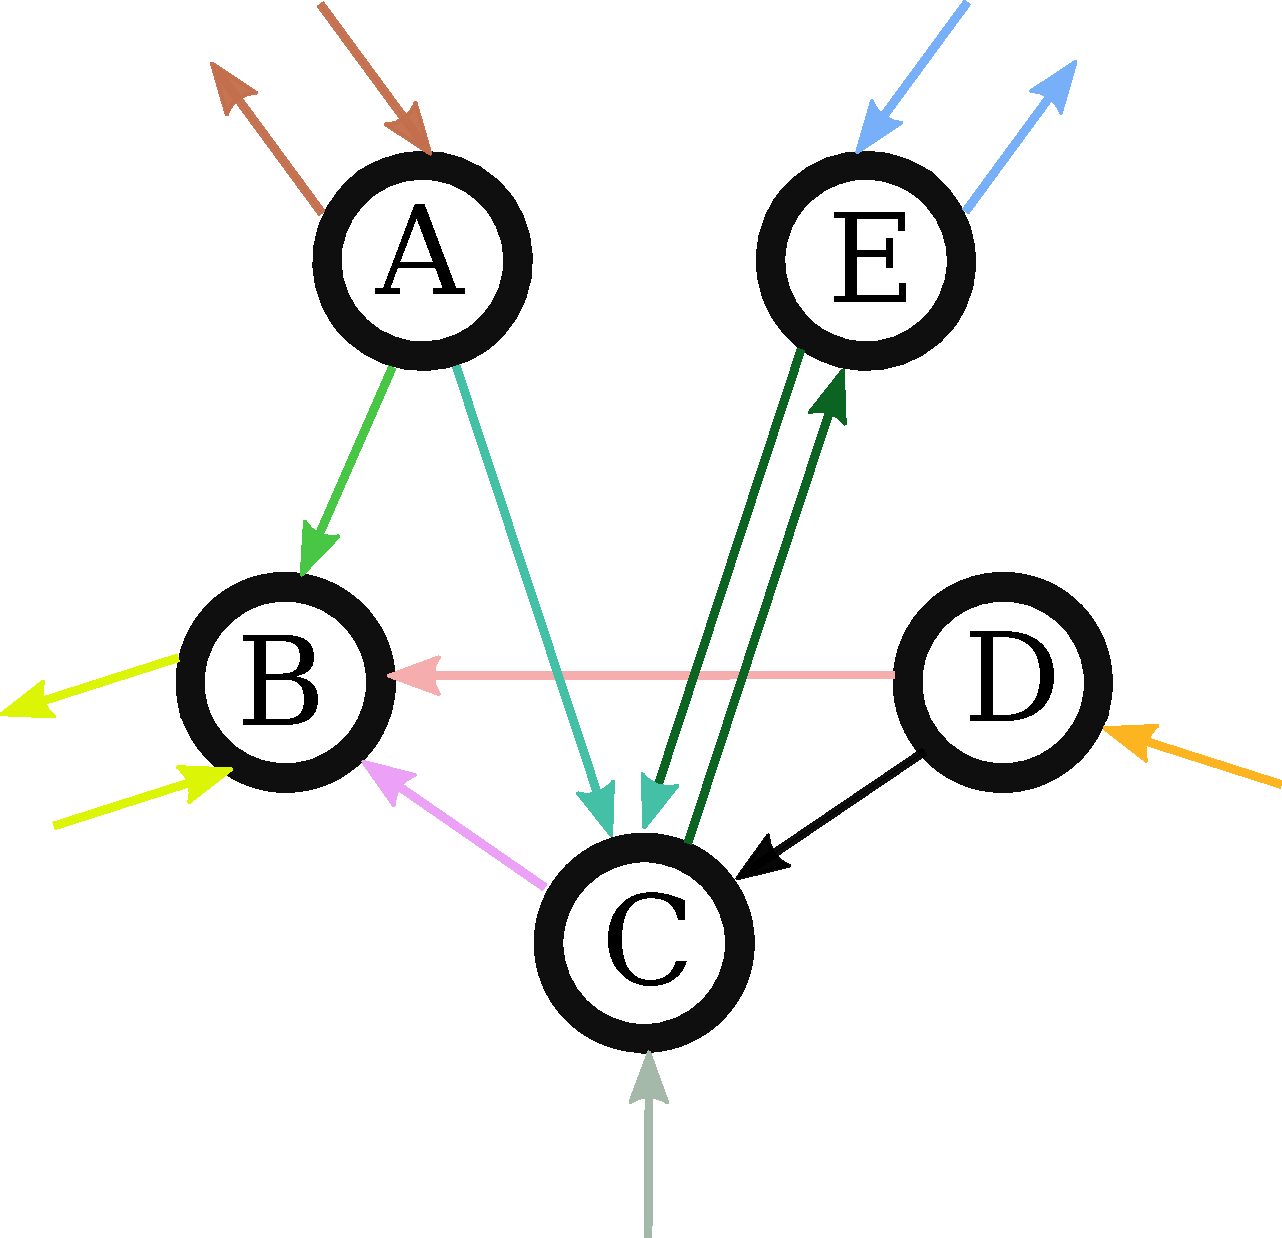
\includegraphics[height=0.9\textheight]{RoundPoolscColoredArrows.pdf}
\end{frame}
%%%%%%%%%%%%%%%%%%%%%%%%%%%%%%%%%%%%%%%%%%%%%%%%%%%%%%%%%%%%%%%%%%%%%%%%%%%%%%%%%%%%%%%%%%%%%%%%%%%%%
\begin{frame}
	\frametitle{}
	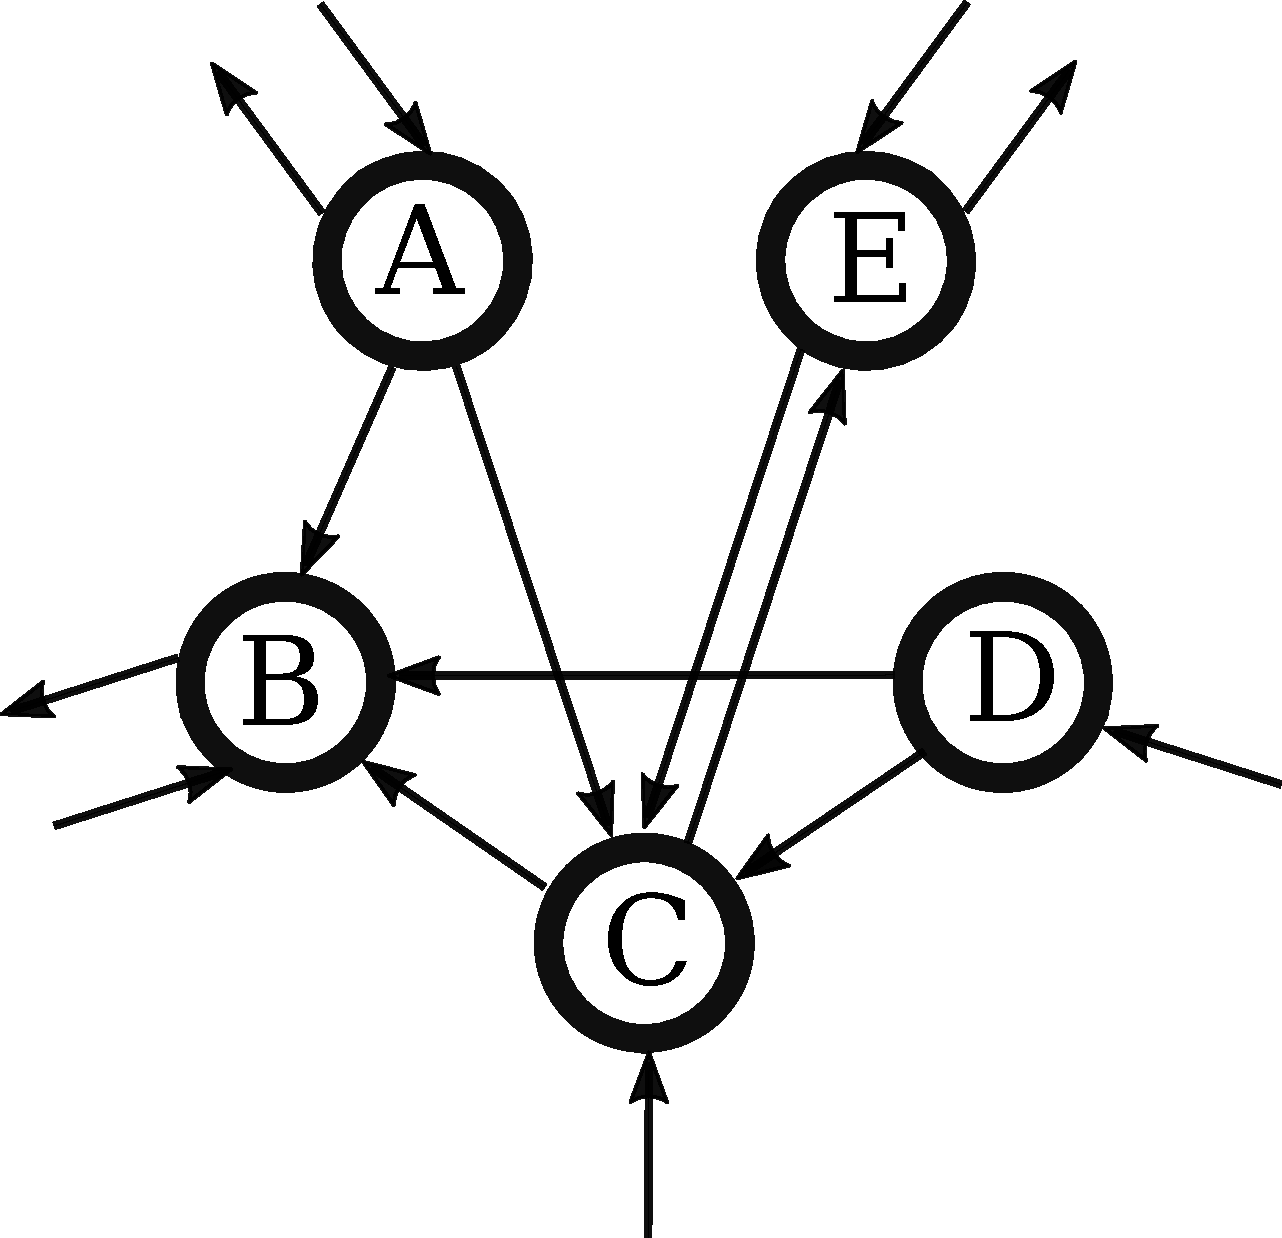
\includegraphics[height=0.9\textheight]{RoundPoolsBlackArrows.pdf}
\end{frame}
%%%%%%%%%%%%%%%%%%%%%%%%%%%%%%%%%%%%%%%%%%%%%%%%%%%%%%%%%%%%%%%%%%%%%%%%%%%%%%%%%%%%%%%%%%%%%%%%%%%%%
\begin{frame}
  
\includegraphics[width=0.45\textwidth]{FritzC.pdf}
  
\includegraphics[width=0.45\textwidth]{Open_passport.pdf}
\end{frame}
%%%%%%%%%%%%%%%%%%%%%%%%%%%%%%%%%%%%%%%%%%%%%%%%%%%%%%%%%%%%%%%%%%%%%%%%%%%%%%%%%%%%%%%%%%%%%%%%%%%%%
\begin{frame}
	\frametitle{}
	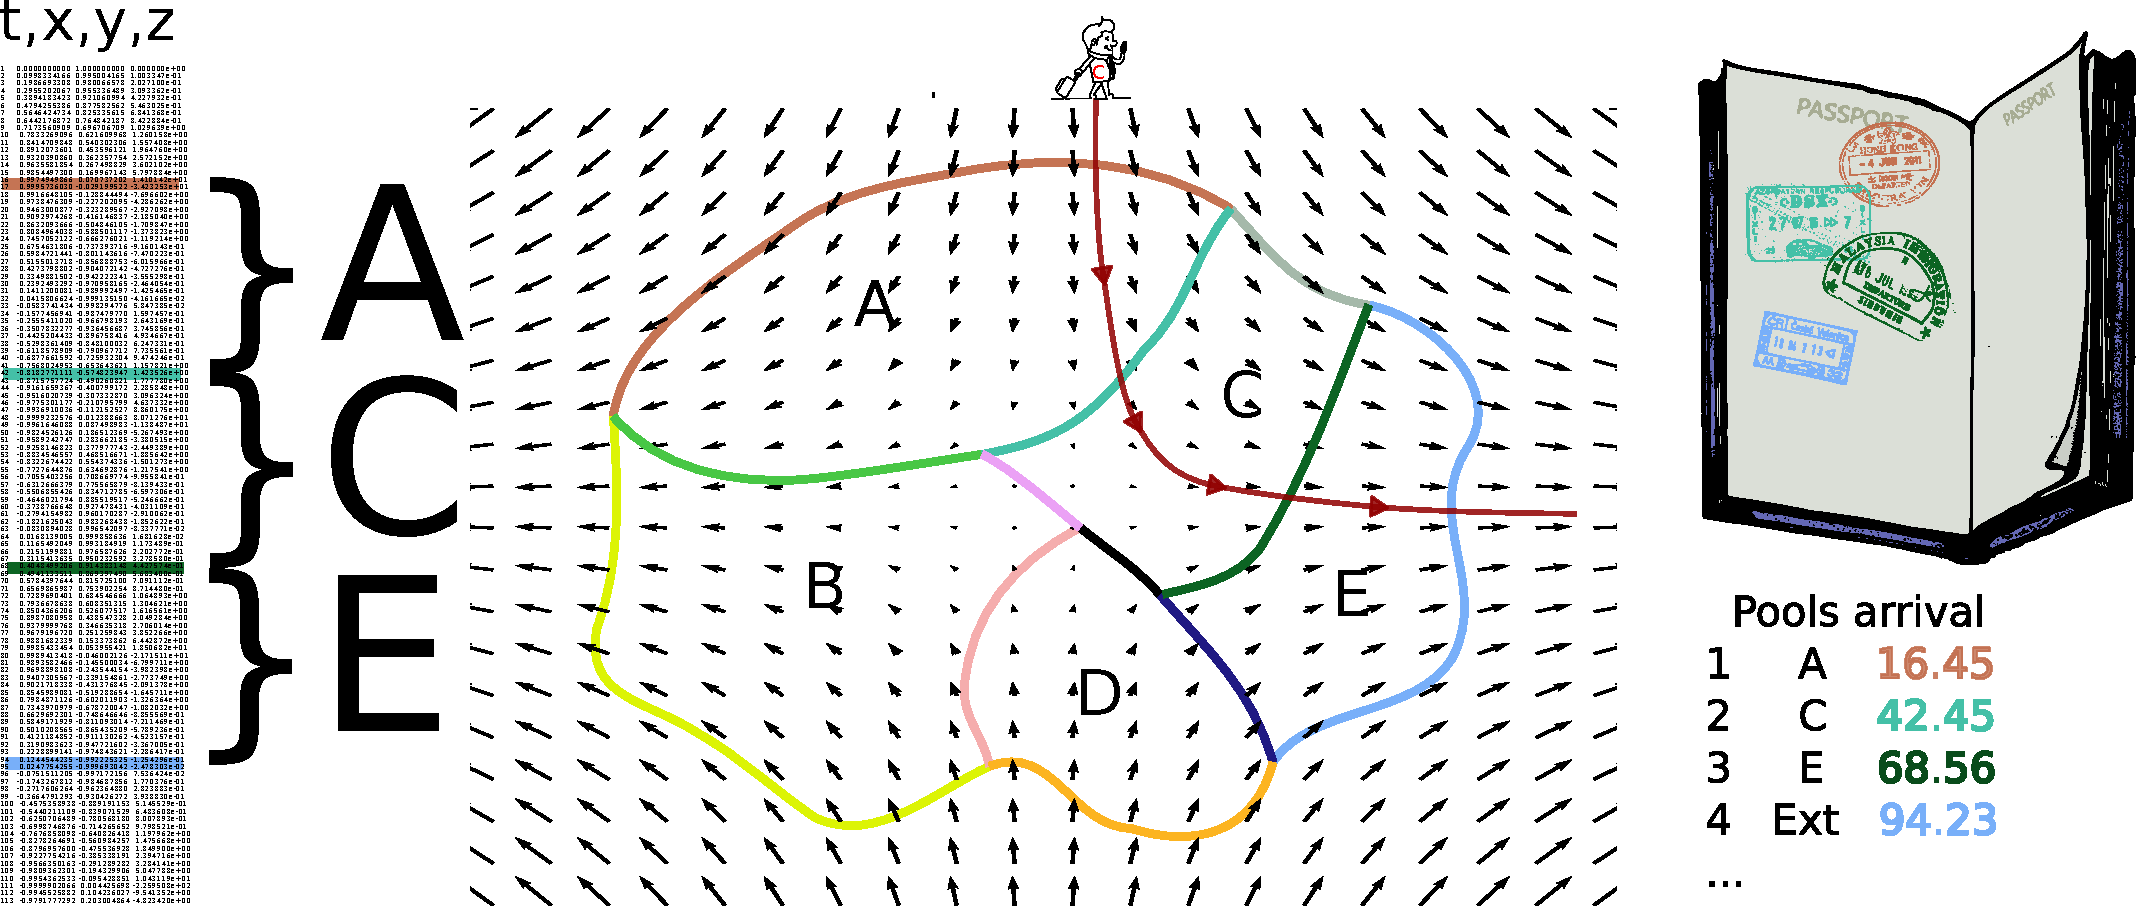
\includegraphics[width=0.9\textwidth]{VectorFieldWithOnePoolAndSubpoolsAndColoredBoundariesAndTrajectory.pdf} 
\end{frame}
%%%%%%%%%%%%%%%%%%%%%%%%%%%%%%%%%%%%%%%%%%%%%%%%%%%%%%%%%%%%%%%%%%%%%%%%%%%%%%%%%%%%%%%%%%%%%%%%%%%%%
\begin{frame}
	\frametitle{}
	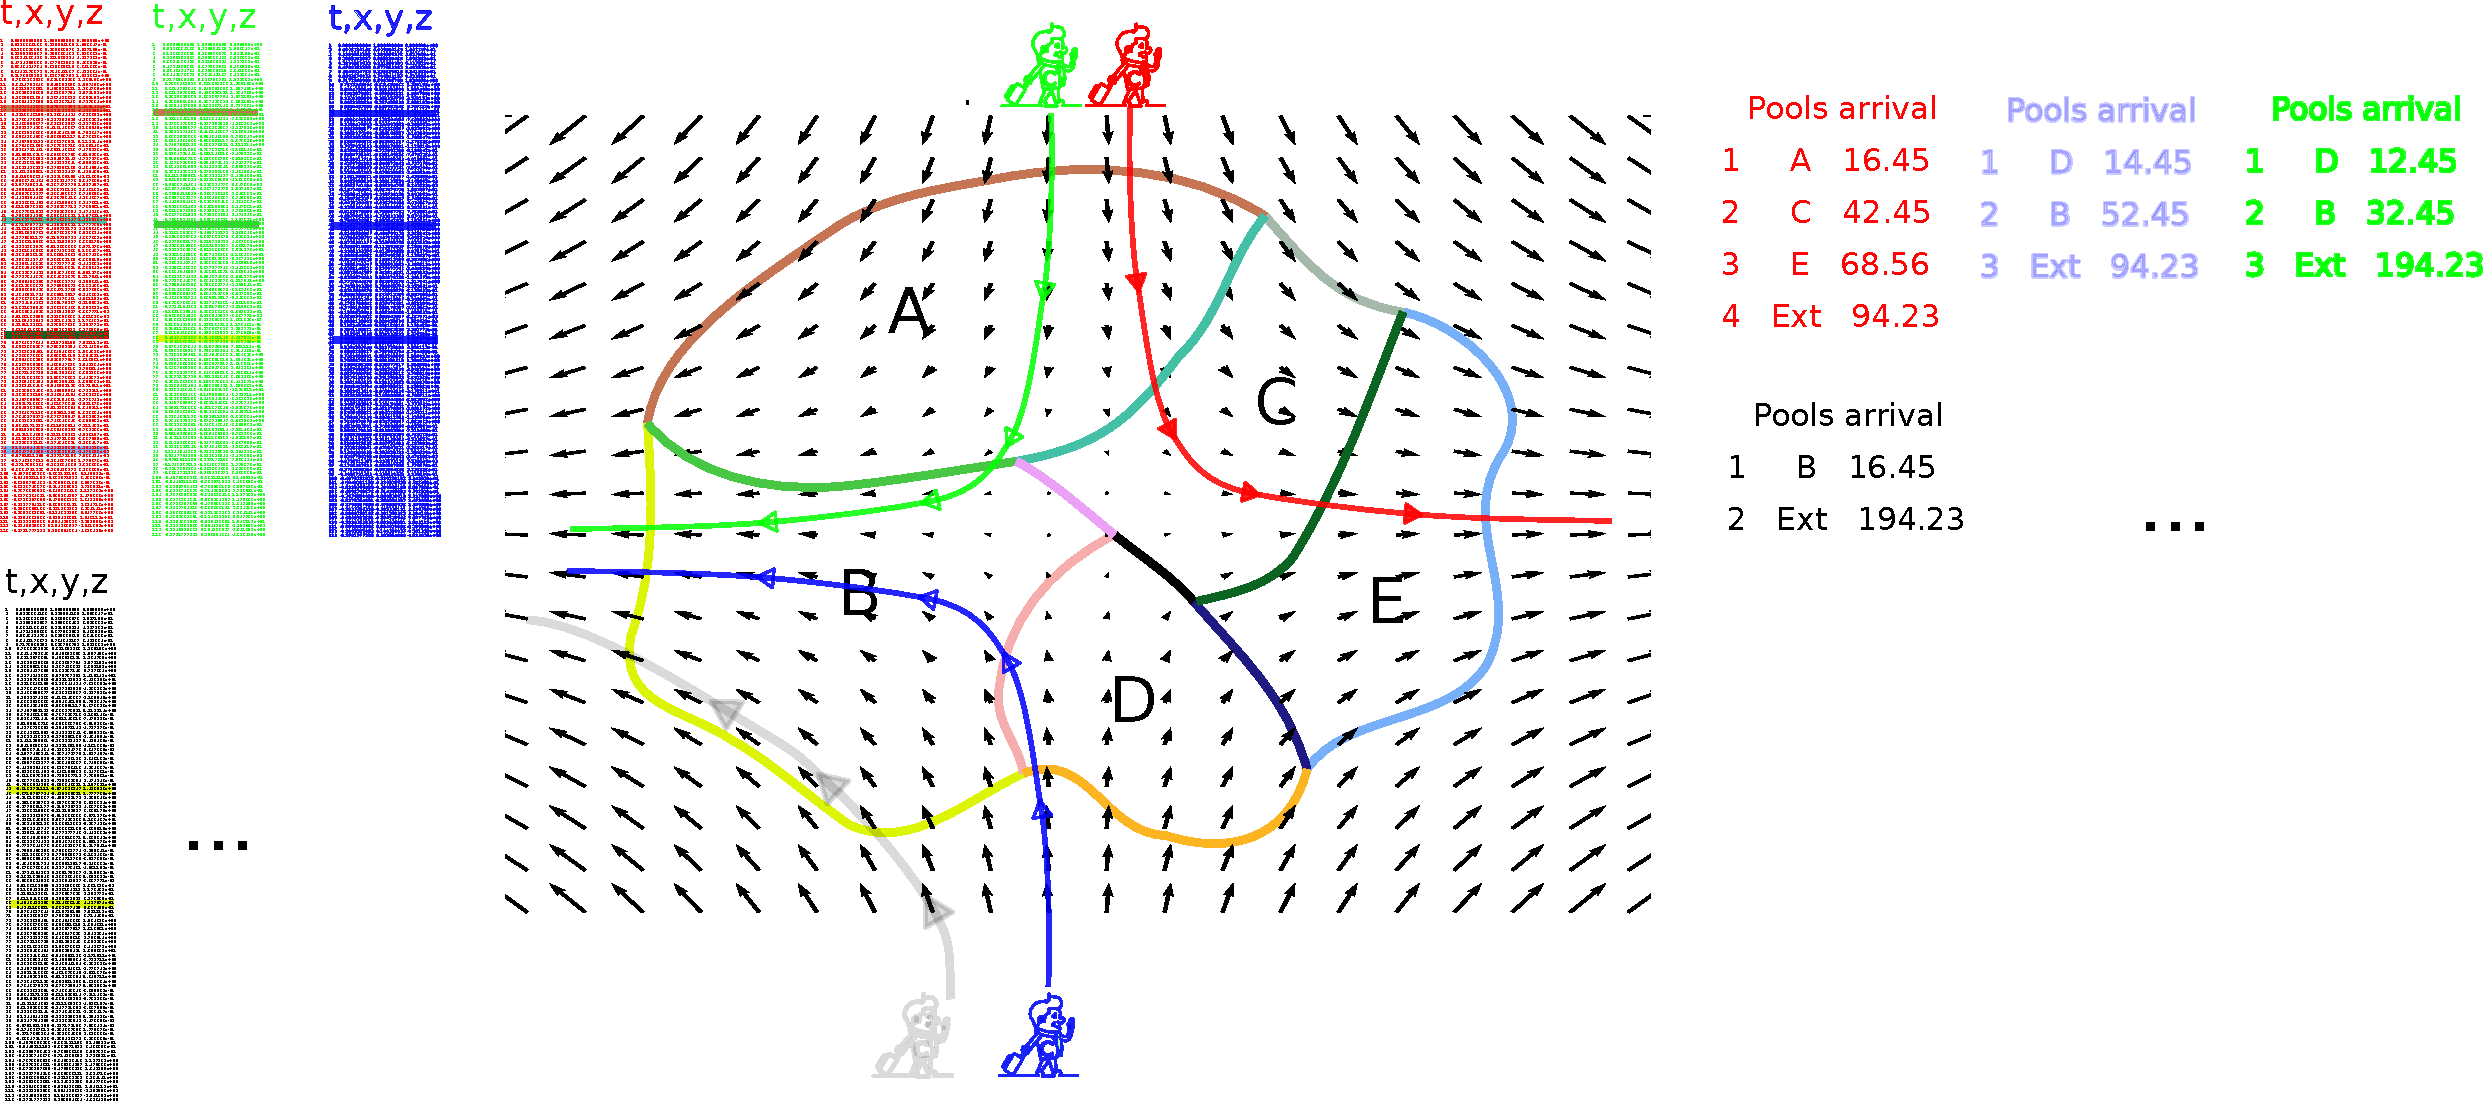
\includegraphics[width=0.99\textwidth]{VectorFieldWithOnePoolAndSubpoolsAndColoredBoundariesAndTrajectories.pdf} 
\end{frame}
%%%%%%%%%%%%%%%%%%%%%%%%%%%%%%%%%%%%%%%%%%%%%%%%%%%%%%%%%%%%%%%%%%%%%%%%%%%%%%%%%%%%%%%%%%%%%%%%%%%%%
\begin{frame}
	\frametitle{Possible  {\color{red} Descriptive} Statistics}
	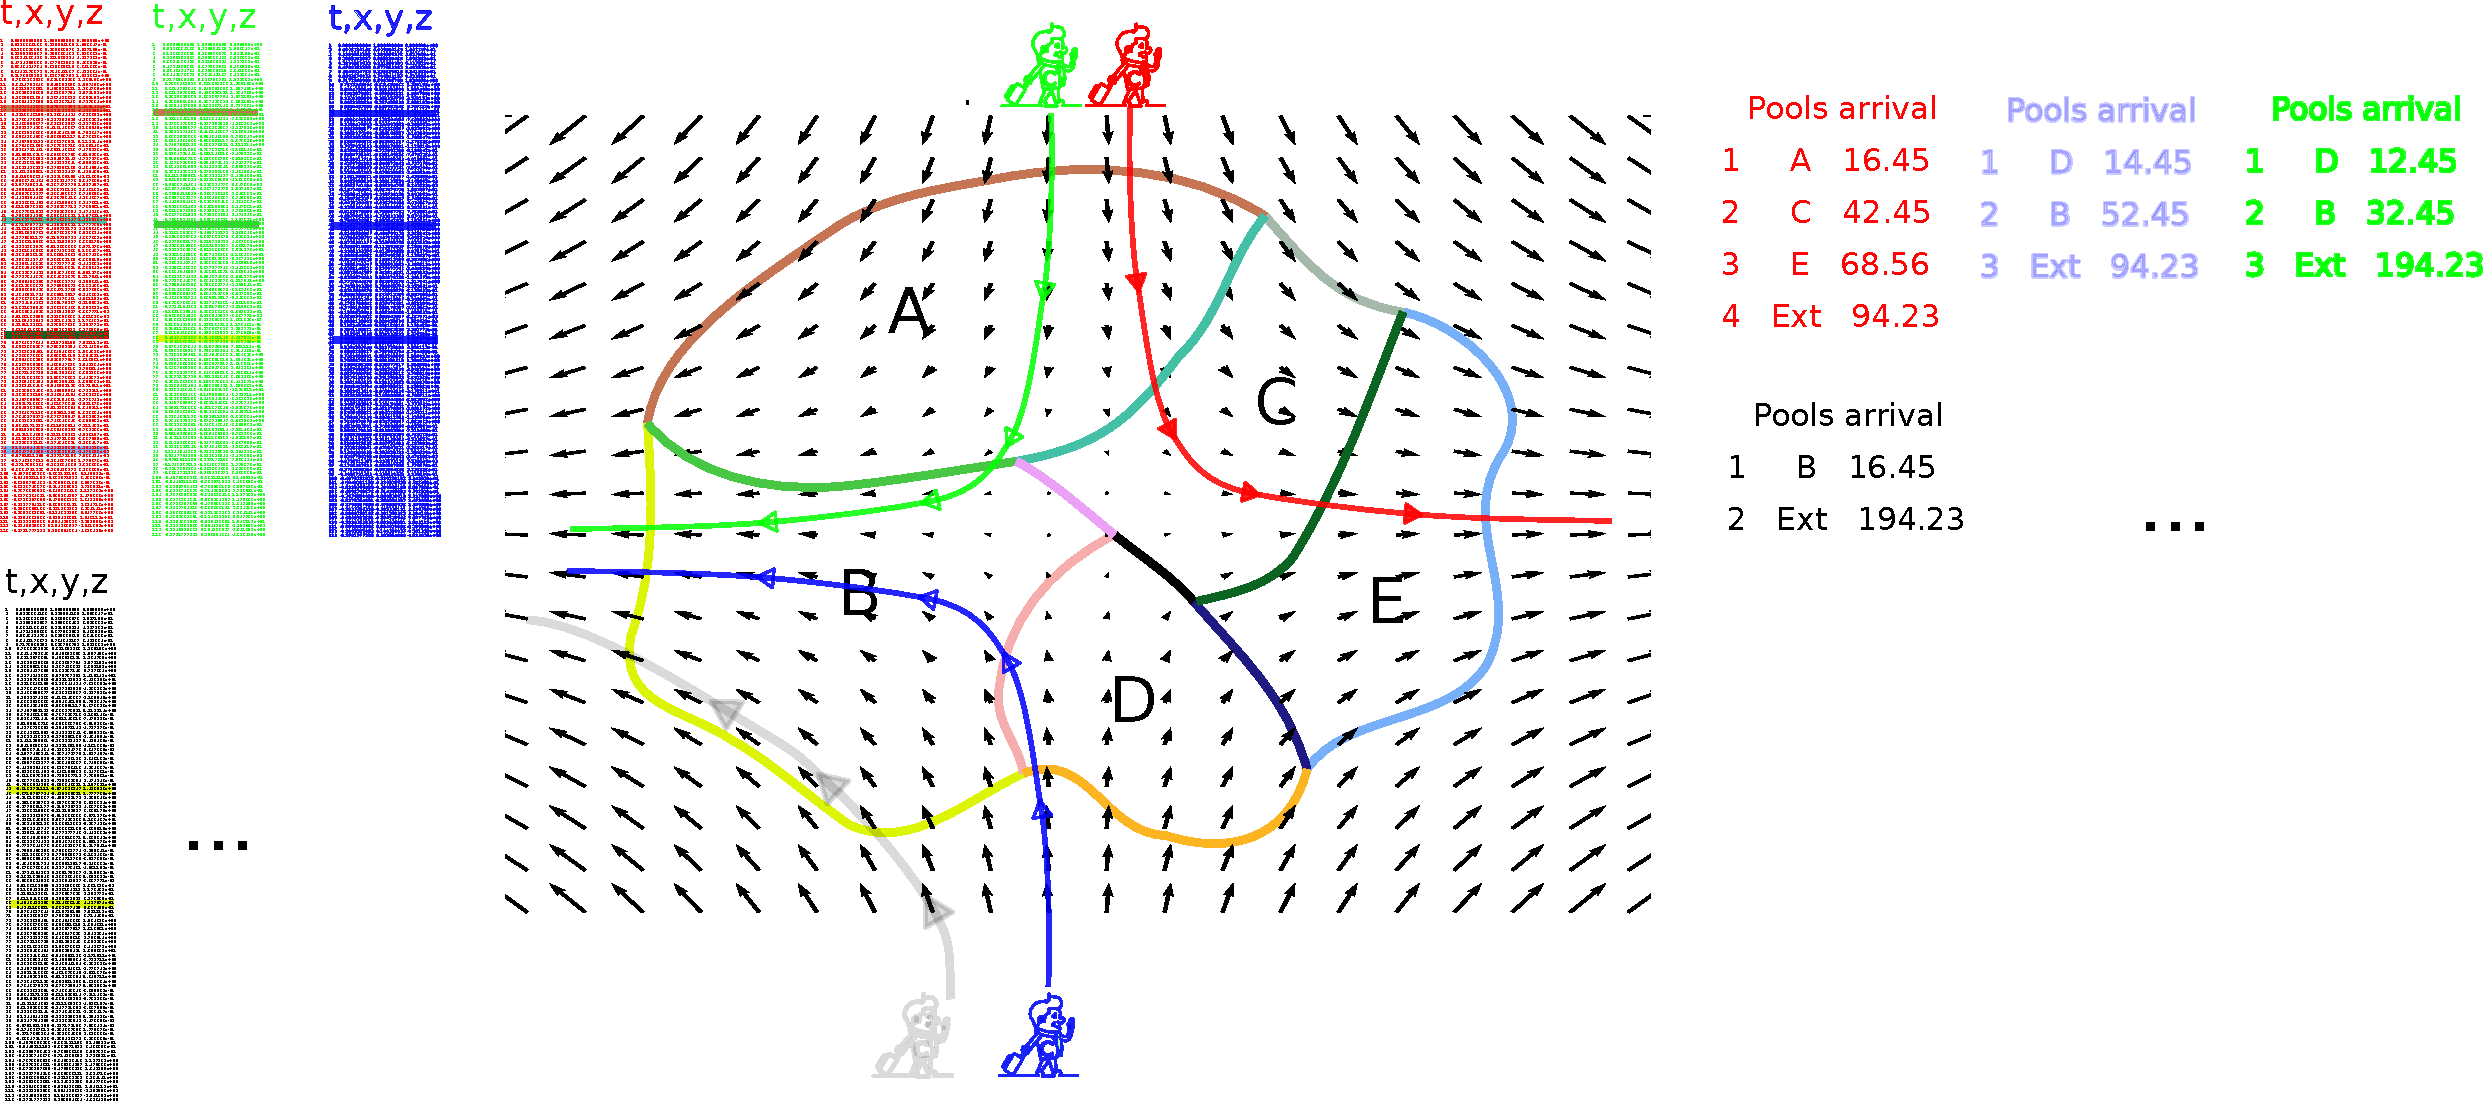
\includegraphics[height=0.45\textheight]{VectorFieldWithOnePoolAndSubpoolsAndColoredBoundariesAndTrajectories.pdf} 
	\begin{itemize}
		\item number / mass of particles in pool A, B, ...
		\item average time spent in a pool A ,B...
		\item average time spent in the whole system 
		\item average time of particles spent between pool C and E under the assumption of having entered by pool D (weird but possible...)
		\item deathrate of pool A.
	\end{itemize}
\end{frame}
%%%%%%%%%%%%%%%%%%%%%%%%%%%%%%%%%%%%%%%%%%%%%%%%%%%%%%%%%%%%%%%%%%%%%%%%%%%%%%%%%%%%%%%%%%%%%%%%%%%%%
\begin{frame}
\frametitle{Age of a Particle}
  \includegraphics<1,2,3>[width=0.6\textwidth]{ParticleAge.pdf}
  \note<1>{
  We can define the age of a particle with respect to the reservoir as the time it has spent in it.
  In the case of the human population this refers to the age in common sense.
  But in general the age refers not to the time of creation but to the time the reservoir was entered.
  If the reservoir in question is e.g. the soil and the particle a $^{14}C$ atom that entered the soil 5 minutes ago
  it is at least 
  possible that the atom is as old as the universe while its age with respect to the soil is only 5 minutes}
  
\begin{itemize}
     \item <2> The ``age '' is always defined in \emph{context} of the reservoir
     \item <3> The ``age '' can not be negative!
\end{itemize}

\end{frame}
%%%%%%%%%%%%%%%%%%%%%%%%%%%%%%%%%%%%%%%%%%%%%%%%%%%%%%%%%%%%%%%%%%%%%%%%%%%%%%%%%%%%%%%%%%%%%%%%%%%%%
\begin{frame}
 [fragile]
\frametitle{Mean Age }
\begin{itemize}
   \item Which set of particles to use for the average?\\ 
      proposition:
      \emph{all} particles that are in the reservoir at the given time. \\
      $\rightarrow$ usually depends on input rates as well as the dynamics of the system.
\end{itemize}
%\begin{tabular}{tt}
  \includegraphics<1>[height=0.3\textheight]{Reservoir_Peoples_Ages.pdf}
  \[
  \bar a(t) =\frac{a_1+a_2+\cdots+a_N}{N}
  \]
  With $N=N(t)$ the number of all particles in the reservoir at time $t$.
%\end{tabular}
  \note{To compute the average age of the population  of the world at a given time we would have to ask everybody how old he is and then compute the mean value.
  If we treat this room as a reservoir everybody would have started a stopwatch entering the room, press the stop button now and we would have to add all the times and divide them by the number of people.}
\end{frame}
%%%%%%%%%%%%%%%%%%%%%%%%%%%%%%%%%%%%%%%%%%%%%%%%%%%%%%%%%%%%%%%%%%%%%%%%%%%%%%%%%%%%%%%%%%%%%%%%%%%%%
\begin{frame}
 [fragile]
\frametitle{Mean Transit Time }
  \includegraphics<1>[height=0.3\textheight]{MeanTransitTime.pdf}
  \[
  \bar t_r(t) =\frac{a_1+a_2+\cdots+a_{n_{o}}}{n_{o}}
  \]
  With $n_{o}=n_{o}(t)$ the number of particles {\color{red} just leaving} at time $t$
\begin{itemize}
   \item Can be time dependent as well
      \pause
   \item Includes only the subset of particles that are just leaving at the given time.
   (Can only be computed when there is an output stream)
   %\item could be independent of input rates and only depend on the dynamics of the system.
\end{itemize}
\note{In the example of the world population it would be sufficient to observe the grave yards.
We would investigate the birth date of every person who dies and compute the average of the live spans. We ignore all the people still alive and concentrate only on the people just dying.
In this room it would be hard to compute the average transit time right now, because nobody is leaving at the moment. (dropping of to sleep does not count as leaving).
But we could after the talk.
Every person would press the stop bottom at its watch in the moment she passes the door.
If two or more people would leave in the same moment we could compute the average of the
times. 
It is also }
\end{frame}
%%%%%%%%%%%%%%%%%%%%%%%%%%%%%%%%%%%%%%%%%%%%%%%%%%%%%%%%%%%%%%%%%%%%%%%%%%%%%%%%%%%%%%%%%%%%%%%%%%%%%
\begin{frame}
 [fragile]
\frametitle{Differences between mean age and mean transit time}
\begin{tabular}{ll}
  \includegraphics<1>[height=0.2\textheight]{Reservoir_Peoples_Ages.pdf} 
  &
  \includegraphics<1>[height=0.2\textheight]{MeanTransitTime.pdf} 
  \\
  \parbox{0.45\textwidth}{
      \begin{itemize}
	 \item Includes { \color{red} all} particles that are in the reservoir at the given time.
         \item Directly coupled to input rates
      \end{itemize}
  }
  &
  \parbox{0.45\textwidth}{
      \begin{itemize}
	 \item Includes only the subset of particles that are {\color{red} just leaving} at the given time.
         \item Indirectly coupled to inputs 
      \end{itemize}
   }
\end{tabular}
\end{frame}
%%%%%%%%%%%%%%%%%%%%%%%%%%%%%%%%%%%%%%%%%%%%%%%%%%%%%%%%%%%%%%%%%%%%%%%%%%%%%%%%%%%%%%%%%%%%%%%%%%%%%
\begin{frame}
 [fragile]
\frametitle{Iteration over all particles}

   \begin{enumerate}
      \item
         To compute the mean transit time we have to identify the particles {\color{red} just leaving}.
      \item
         Ask every leaving  particle   when it entered and compute its age.
      \item
         Iterate over all particles and compute the average of their ages.
      \pause
     \[
     \bar t_r(t) =\frac{a_1+a_2+\cdots+a_{n_{o}}}{n_{o}}
     \]
     With $n_{o}=n_{o}(t)$ the number of particles just leaving at time $t$
   \end{enumerate}
\begin{knitrout}\footnotesize
\definecolor{shadecolor}{rgb}{0.969, 0.969, 0.969}\color{fgcolor}

{\centering 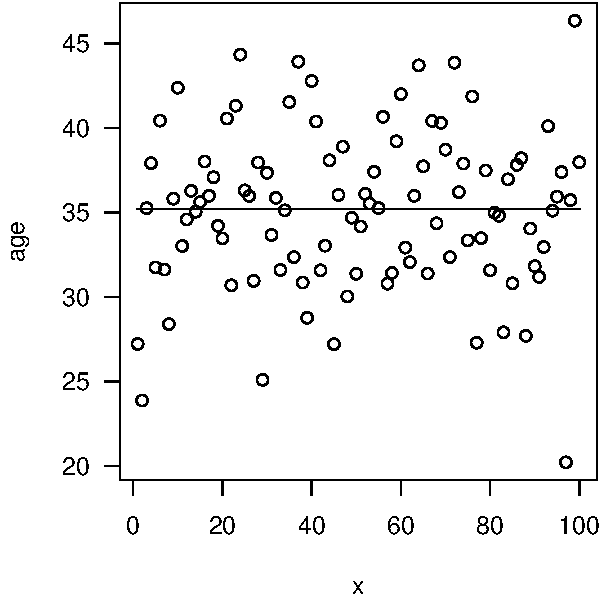
\includegraphics[width=.4\linewidth]{figure/beamer-mean-1} 

}



\end{knitrout}
\end{frame}
%%%%%%%%%%%%%%%%%%%%%%%%%%%%%%%%%%%%%%%%%%%%%%%%%%%%%%%%%%%%%%%%%%%%%%%%%%%%%%%%%%%%%%%%%%%%%%%%%%%%%%
\begin{frame}
 [fragile]
   \frametitle{Iteration over all {\color{red} ages}}
\begin{enumerate}
   \item as above
   \item as above + make a histogram of all ages
   \item iterate over all ages and compute their weighted average
      \pause
     \[
     \bar t_r(t) =\frac{a_1 n_{a_1} +a_2 n_{a_2} +\cdots+a_{n}n_{a_n}}{n_{o}}
     \]
     With $n_{o}=n_{o}(t)=n_{a_1} + n_{a_2} +\cdots +n_{a_n}$ 
   \end{enumerate}
\begin{knitrout}\footnotesize
\definecolor{shadecolor}{rgb}{0.969, 0.969, 0.969}\color{fgcolor}

{\centering 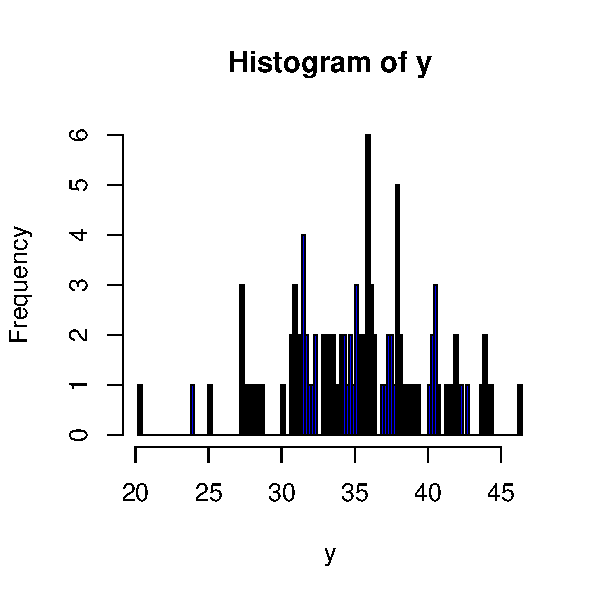
\includegraphics[width=.35\linewidth]{figure/beamer-histogram-1} 

}



\end{knitrout}
\end{frame}
%%%%%%%%%%%%%%%%%%%%%%%%%%%%%%%%%%%%%%%%%%%%%%%%%%%%%%%%%%%%%%%%%%%%%%%%%%%%%%%%%%%%%%%%%%%%%%%%%%%%%%
\begin{frame}
 [fragile]
   \frametitle{Integration over a {\color{red}density}}
\begin{eqnarray*}
     \bar t_r(t) &=&\lim_{n\to \infty} \frac{a_1 n_{a_1} +a_2 n_{a_2} +\cdots+a_{n}n_{a_n}}{n_{o}}
     \\
     &=&\lim_{n\to \infty}\sum_{minage}^{maxage} a \frac{n(a)}{n_o} da
     \\
     &=&\int_{minage}^{maxage} a \psi(a) da
\end{eqnarray*}
\begin{knitrout}\footnotesize
\definecolor{shadecolor}{rgb}{0.969, 0.969, 0.969}\color{fgcolor}

{\centering 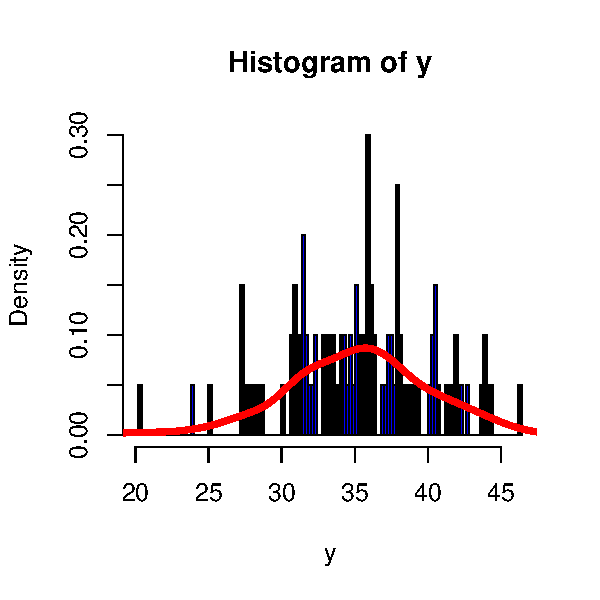
\includegraphics[width=.35\linewidth]{figure/beamer-dens-1} 

}



\end{knitrout}
\end{frame}
%%%%%%%%%%%%%%%%%%%%%%%%%%%%%%%%%%%%%%%%%%%%%%%%%%%%%%%%%%%%%%%%%%%%%%%%%%%%%%%%%%%%%%%%%%%%%%%%%%%%%%
\begin{frame}
 [fragile]
 \frametitle{Same procedure for {\color{red} age} density}
\begin{eqnarray*}
     \bar a(t) &=&\lim_{n\to \infty} \frac{a_1 n_{a_1} +a_2 n_{a_2} +\cdots+a_{n}n_{a_n}}{n_{p}}
     \\
     &=&\lim_{n\to \infty}\sum_{minage}^{maxage} a \frac{n(a)}{n_p} da
     \\
     &=&\int_{minage}^{maxage} a \phi(a) da
\end{eqnarray*}
\begin{knitrout}\footnotesize
\definecolor{shadecolor}{rgb}{0.969, 0.969, 0.969}\color{fgcolor}

{\centering 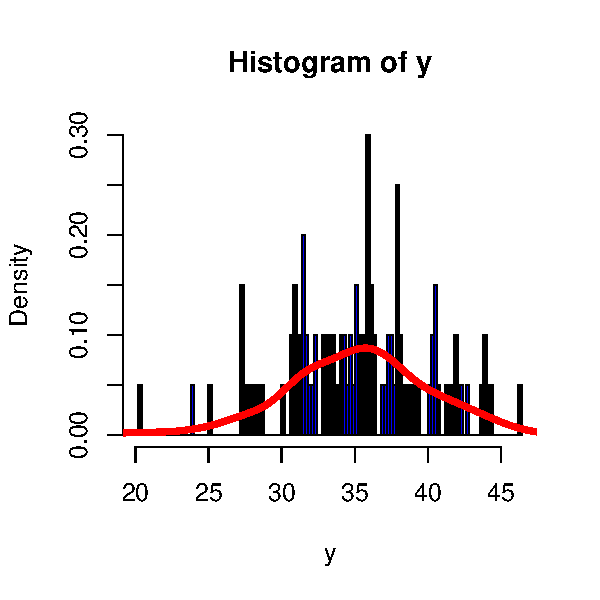
\includegraphics[width=.35\linewidth]{figure/beamer-dens2-1} 

}
\end{knitrout}
\end{frame}
%%%%%%%%%%%%%%%%%%%%%%%%%%%%%%%%%%%%%%%%%%%%%%%%%%%%%%%%%%%%%%%%%%%%%%%%%%%%%%%%%%%%%%%%%%%%%%%%%%%%%
\subsection{Answer Questions more simply}
%%%%%%%%%%%%%%%%%%%%%%%%%%%%%%%%%%%%%%%%%%%%%%%%%%%%%%%%%%%%%%%%%%%%%%%%%%%%%%%%%%%%%%%%%%%%%%%%%%%%%
\begin{frame}
	\frametitle{Possible {\color{red} Predictive} Statistics ?}
	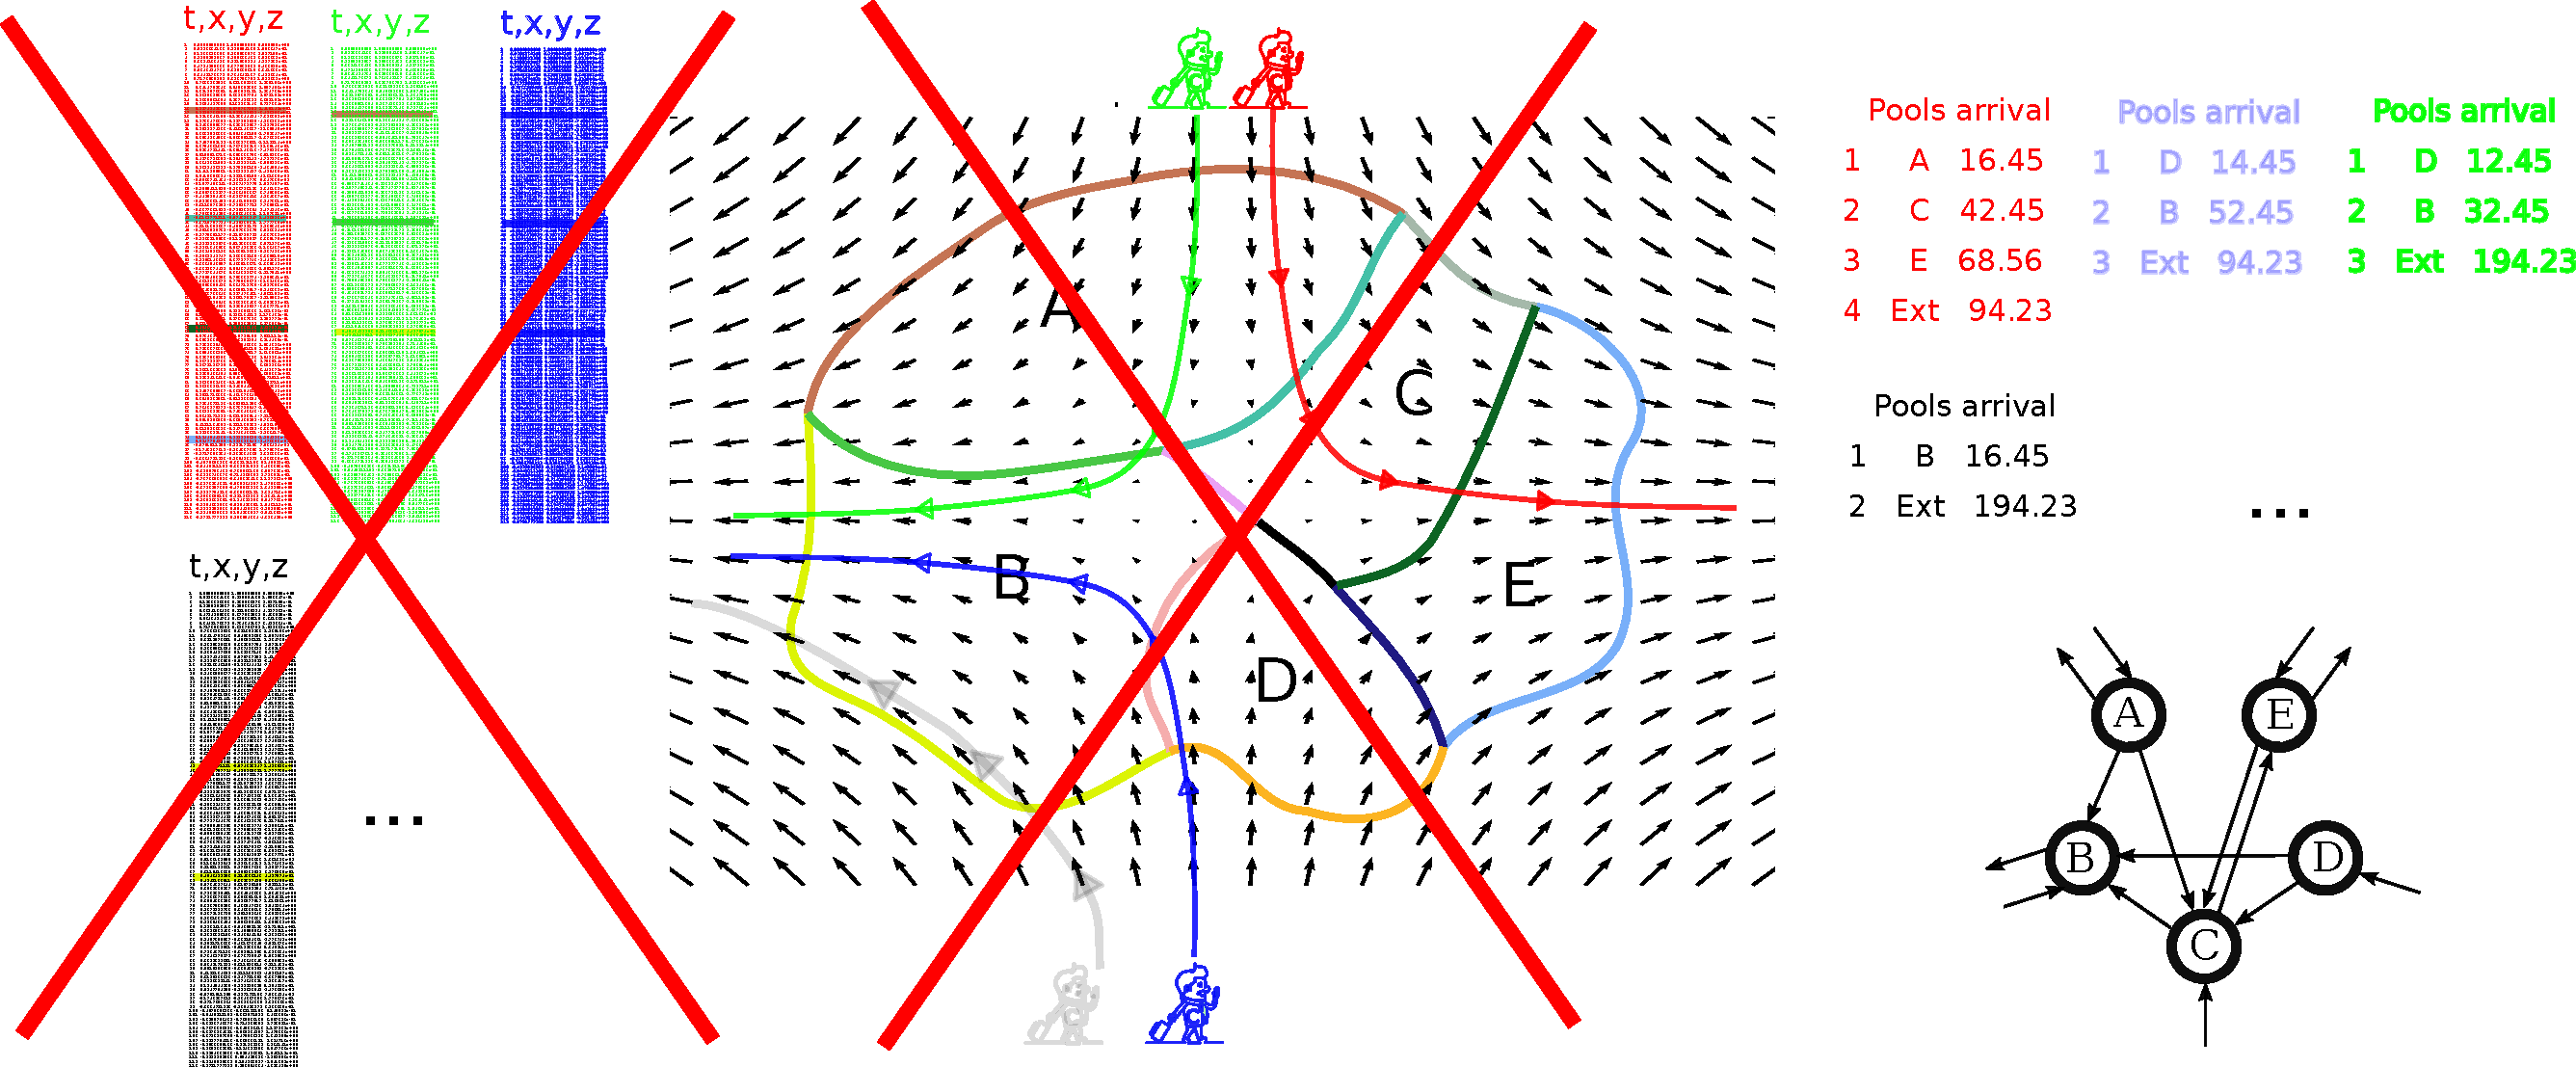
\includegraphics[height=0.45\textheight]{VectorFieldWithOnePoolAndSubpoolsAndColoredBoundariesAndCrossedTrajectories.pdf} 
	\begin{itemize}
	\item
		Could we make a rule to predict the number of particles exiting from Pool E at time using only the particle passports? (Assuming that the exit from E is not recorded.)  
	\item
		Could we make a rule to predict the age distribution of particles exiting from Pool E at time using only the particle passports? (Assuming again that the exit from E is not recorded.)  

	\end{itemize}
\end{frame}

%%%%%%%%%%%%%%%%%%%%%%%%%%%%%%%%%%%%%%%%%%%%%%%%%%%%%%%%%%%%%%%%%%%%%%%%%%%%%%%%%%%%%%%%%%%%%%%%%%%%%
\begin{frame}
	\frametitle{Intermediate Summary}
	\begin{enumerate}
	\item
		Pool descriptions condense complex information to a time series of pool changes.(A series of stamps in the passport)
	\item 
		There are many possible statistics on sets of these time series,
		usually related to numbers of particles and times.
		(e.g. the number of particles in a pool, 
		
	\item 
		Pool {\color{red} Models} predict = model some of these {\color{red} exclusively} with respect to 
			the information obtainable from (all) passports. 
	\item  
		The most common even disregard most of the information in the passports.
		

	\end{enumerate}
\end{frame}
%%%%%%%%%%%%%%%%%%%%%%%%

\frame{
\frametitle{Diverse model predictions}
\begin{center}
  \begin{multicols}{2}
    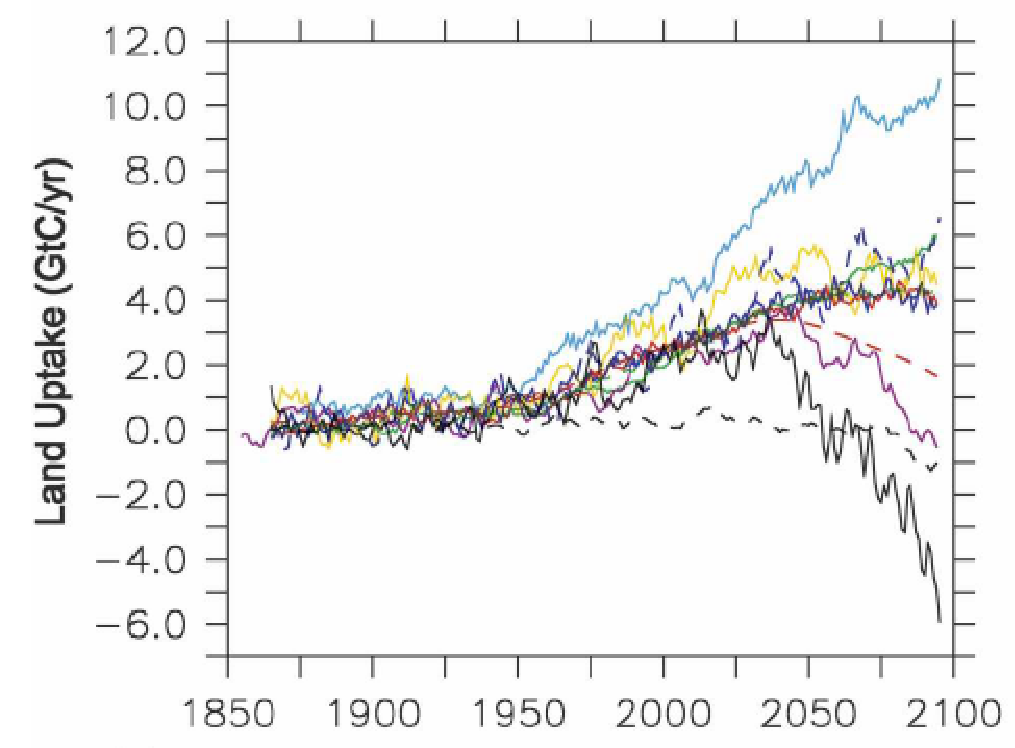
\includegraphics[scale=0.3]{Figures/Fried1} \\
    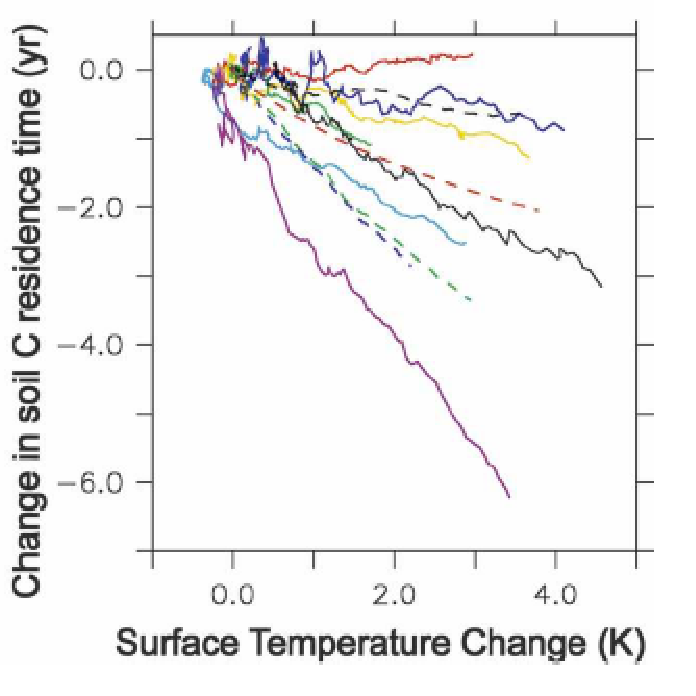
\includegraphics[scale=0.35]{Figures/Fried2}
  \end{multicols}
  \tiny{\citet{Friedlingstein2006JC}}
\end{center}
}

%%%%%%%%%%%%%%%%%%%%%%%%
\frame{
\frametitle{Model comparison}
\bf{Key quantities}\vspace{1cm}
\begin{itemize}
  \item<2 -> transit time
    \begin{itemize}
      \item the time that particles need to travel through the system
      \item exit time - entry time
    \end{itemize}
  \item<3 -> system age
    \begin{itemize}
      \item for particles in the system
      \item current time - entry time
    \end{itemize}
  \item<4-> compartment age
    \begin{itemize}
      \item system age of particles in a compartment
    \end{itemize}
\end{itemize}
}

%%%%%%%%%%%%%%%%%%%%%%%%

\frame{
\frametitle{Linear autonomous compartmental models}
\begin{figure}[htbp]
  \begin{minipage}{0.4\textwidth}
  \hspace{1cm}
  $\frac{d}{dt}\,\vec{x}(t) = \tens{A}\,\vec{x}(t) + \vec{u}$
  \end{minipage}
  \hfill
  \begin{minipage}{0.55\textwidth}
    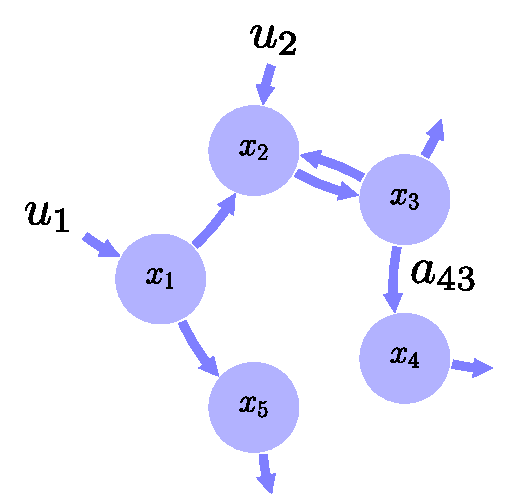
\includegraphics[scale=0.35]{Figures/ModelLogo}
  \end{minipage}  
\end{figure} 

{\renewcommand{\arraystretch}{1.5}
\begin{tabular}{ll}
  \pause $\vec{x}(t)$ & vector of compartment content (e.g. C) at time $t$\\
  \pause $\vec{u}$ & constant input vector\\
  \pause $\tens{A}=(a_{ij})$ & compartmental matrix\\
  \pause $a_{ij}\,(i\neq j)$ & fractional transfer coefficients,\\
  & rate of flow from compartment $j$ to compartment $i$ \\
  \pause $-a_{ii}>0$ & rate of flow out of compartment $i$
\end{tabular}
}
}

%%%%%%%%%%%%%%%%%%%%%%%%

% \frame{
% \frametitle{Existing results}
% \bf{Existing results for transit time and age}\vspace{1cm}
% \begin{itemize}
%   \item<1 -> formulas for means \citep{Rasmussen2016JMB}
%   \begin{itemize}
%     \item <2 -> \color[rgb]{1,0,0}no consideration of deviations from ideal behavior possible
%   \end{itemize}
% 
%   \item<3 -> numerical computations of densities \citep{Thompson1999GCB}
%   \begin{itemize}
%     \item<4 -> \color[rgb]{1,0,0}costly long-time simulation
%   \end{itemize}
%   \item<5 -> formulas for densities \citep{Manzoni2009JGR}
%   \begin{itemize}
%     \item<6 -> \color[rgb]{1,0,0}only models with very simple structure
%     \item<7 -> \color[rgb]{1,0,0}difficult case-by-case computation
%     %\item<8 -> transformation of impulsive inputs to Laplace domain and back
%   \end{itemize}
% \end{itemize}
% }

%%%%%%%%%%%%%%%%%%%%%%%%%%%%

% \frame{
% \frametitle{Goals}
% \bf{Stochastic approach}\vspace{1cm}
% \begin{itemize}
%   \item<2 -> represent compartmental model by {\color[rgb]{1,0,0}stochastic process}: continuous-time Markov chain
%   \item<3 -> find {\color[rgb]{1,0,0}general, simple, explicit} density formulas
%   \item<4 -> (re)open stochastic toolbox to carbon cycle modeling
% \end{itemize}
% 
% }

%%%%%%%%%%%%%%%%%%%%%%%%

% \frame{
% \frametitle{One-particle perspective}
% Instead of entire masses we consider one single particle:
% \vspace{1cm}
% \begin{itemize}
%   \item<2-> enters the system at a pool according to input vector $\vec{u}$
%   \item<3-> travels through and leaves system according to compartmental matrix $\tens{A}$
%   \item<4-> path represented by stochastic process
%   \begin{itemize}
%     \item linear autonomous system: continuous-time Markov chain
%   \end{itemize}
%   \item<5->[$\to$] probability density functions of this particle reflect distribution of mass in the system.
% 
% \end{itemize}
% }

%%%%%%%%%%%%%%%%%%%%%%%%

\frame{
\frametitle{A particle travels \hspace{3cm} $\frac{d}{dt}\,\vec{x}(t)=\tens{A}\,\vec{x}(t)+\vec{u}$}

%\begin{center}
  \begin{minipage}[t]{1.0\textwidth}
    \begin{minipage}{0.35\textwidth}
      \vspace{-1cm}
      \includegraphics<1>[scale=0.5]{Figures/system_empty.pdf}
      \includegraphics<2>[scale=0.5]{Figures/system_T0.pdf}
      \includegraphics<3>[scale=0.5]{Figures/system_T1-T0.pdf}
      \includegraphics<4>[scale=0.5]{Figures/system_T1.pdf}
      \includegraphics<5>[scale=0.5]{Figures/system_T2-T1.pdf}
      \includegraphics<6>[scale=0.5]{Figures/system_T2.pdf}
      \includegraphics<7>[scale=0.5]{Figures/system_T3-T2.pdf}
      \includegraphics<8>[scale=0.5]{Figures/system_T3.pdf}
      \includegraphics<9>[scale=0.5]{Figures/system_T4-T3.pdf}
      \includegraphics<10>[scale=0.5]{Figures/system_T4.pdf}
      \includegraphics<11>[scale=0.5]{Figures/system_end.pdf}
    \end{minipage}
    \hfill
    \begin{minipage}{0.6\textwidth}
      \vspace{-0.2cm}
      \begin{tabular}{rcc}
        &$\tens{A}$ & $\vec{u}$ \\
        & \\
        
	&$\begin{pmatrix}
	    \colorize<3,7>-a_{11} & \colorize<6>a_{12} & \colorize<10>0 \\
	    \colorize<4,8>a_{21} & \colorize<5>-a_{22} & \colorize<10>0 \\
	    \colorize<4,8>a_{31} & \colorize<6>0 & \colorize<9>-a_{33}\\
	\end{pmatrix}$
	&
	$\begin{pmatrix} \colorize<2>u_1 \\ \colorize<2>u_2 \\ 0 \end{pmatrix}$ \\
	\\
	$-\sum$ & $\begin{matrix} \colorize<4,8>0 & \quad\colorize<6> >0 & \quad\colorize<10> >0\end{matrix}$ & $\|\vec{u}\|$
      \end{tabular}
      \vspace{1cm}
      
      \begin{tabular}{cc}
	\only<1,3,5,7,9,11>{\uncover<0>{$p_{12} = \frac{3}{4}$ &}}
	\only<2>{\red{$\beta_1 = \frac{u_1}{u_1+u_2}$}
	&
	\red{$\beta_2 = \frac{u_2}{u_1+u_2}$}}

	\only<4>{\red{$p_{21} = \frac{a_{21}}{a_{11}}$}
	&
	\red{$p_{31} = \frac{a_{31}}{a_{11}}$}}

	\only<6>{\red{$p_{12} = \frac{a_{12}}{a_{22}}$}
	&
	\red{$p_{02} = 1-\frac{a_{12}}{a_{22}}$}}

	\only<8>{\red{$p_{21} = \frac{a_{21}}{a_{11}}$}
	&
	\red{$p_{30} = \frac{a_{31}}{a_{11}}$}}

	\only<10>{\red{$p_{03} = 1$}
	&
	}

      \end{tabular}
    \end{minipage}
  \end{minipage}
%\end{center}

\includegraphics<1>[scale=0.6]{Figures/timeline_empty.pdf}
\includegraphics<2>[scale=0.6]{Figures/timeline_T0.pdf}
\includegraphics<3>[scale=0.6]{Figures/timeline_T1-T0.pdf}
\includegraphics<4>[scale=0.6]{Figures/timeline_T1.pdf}
\includegraphics<5>[scale=0.6]{Figures/timeline_T2-T1.pdf}
\includegraphics<6>[scale=0.6]{Figures/timeline_T2.pdf}
\includegraphics<7>[scale=0.6]{Figures/timeline_T3-T2.pdf}
\includegraphics<8>[scale=0.6]{Figures/timeline_T3.pdf}
\includegraphics<9>[scale=0.6]{Figures/timeline_T4-T3.pdf}
\includegraphics<10>[scale=0.6]{Figures/timeline_T4.pdf}
\includegraphics<11>[scale=0.6]{Figures/timeline.pdf}
}

%%%%%%%%%%%%%%%%%%%%%%%

% \frame{ 
% \frametitle{Absorbing continuous-time Markov chain}
% \begin{itemize} 
%   \item<1-> path of particle represented by stochastic process $(X_t)_{t\geq0}$
%   \item<2-> $X_t=k$ if particle in compartment $k$ at time $t$
%   \item<3-> $X_t=0$ if particle has left the system
%   \item<4-> future of particle
%   \begin{itemize}
%     \item depends only on current position
%     \item independent of past
%     \item[$\to$] Markov property
%   \end{itemize}
%   \item<5-> $X=(X_t)_{t\geq0}$ \red{continuous-time Markov chain}
%   \begin{itemize}
%     \item $0$ is absorbing state (will never be left)
%     \item if $\tens{A}$ invertible, absorbing state will be reached
%     \item[$\to$] $X$ is called \red{absorbing}
%   \end{itemize}
% \end{itemize}
% }

%%%%%%%%%%%%%%%%%%%%%%%%

\frame{
\frametitle{Transit time distribution}
\begin{itemize}
  \item<1-> transit time computation:
    \[
      T = \underbrace{(T_1-T_0)}_{\sim \Exp(a_{11})} + \underbrace{(T_2-T_1)}_{\sim \Exp(a_{22})} + \underbrace{(T_3-T_2)}_{\sim \Exp(a_{11})} + \underbrace{(T_4-T_3)}_{\sim \Exp(a_{33})}
    \]
  \item<2-> mixture of exponential distributions
  \item<3-> length of mixture is stochastic
  \item<4->[$\to$] $T$ follows \red{phase-type distribution} with parameters $\vec{\beta}$, $\tens{A}$
  \item<5->[] $\vec{\beta} = \frac{\vec{u}}{\|\vec{u}\|}$
  \item<6->[$\to$] $T\sim\operatorname{PH}(\vec{\beta},\tens{A})$
\end{itemize}
}

%%%%%%%%%%%%%%%%%%%%%

% \frame{
% \frametitle{Phase-type distribution}
% \begin{itemize} 
%   \item <1-> describes transit time $T$
%   \item <2-> mixture of exponential distributions
%   \item <3-> probability density function:
%     \[
%       f_T(t) = \vec{z}^T\, e^{t\,\tens{A}}\,\vec{\beta},\quad t\geq0.
%     \]
%   \item <4-> expected value:
%     \[
%       \E[T] = -\vec{1}^T\, \tens{A}^{-1}\,\vec{\beta} = \|\tens{A}^{-1}\,\vec{\beta}\|,
%     \]
%   \item <5-> higher order moments:
%     \[
%       \E[T^n] = (-1)^n\,n!\,\vec{1}^T\, \tens{A}^{-n}\,\vec{\beta}.
%     \]
% \end{itemize}
% }

%%%%%%%%%%%%%%%%%%%%%

% \frame{
% \frametitle{Renewal process for age}
% \begin{itemize}
%   \item<1-> need infinite history (no maximum age)
%   \item<1->[$\to$] particle reenters system after leaving it
%   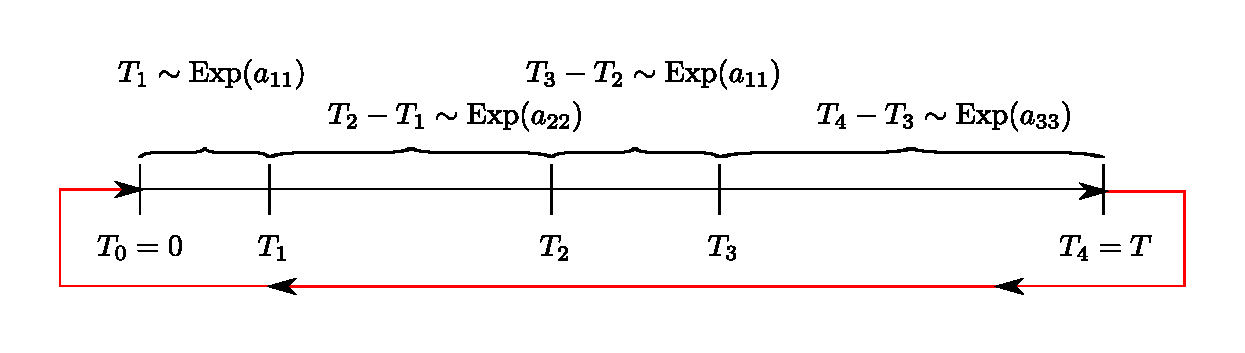
\includegraphics[scale=0.5]{Figures/cycles_single.pdf}
%   \vspace{-0.25cm}
%   \item<2->[$\to$] infinite number of cycles
%   
\includegraphics[width=10cm,height=1cm]{Figures/cycles_infinite.pdf}
%   \vspace{-0.25cm}
%   \item<2-> \emph{system age} = time since last restart at random time
%   \item<2-> \emph{compartment age} = time since last restart at random time given particle is in certain compartment
% \end{itemize}
% }

% \frame{
% \frametitle{System age and pool age densities}
% \bf{Steady state formulas}\vspace{1cm}
% \begin{itemize}
%   \item<2-> system age density 
%     \[
%       f_A(y) = \vec{z}^T\, e^{y\,\tens{A}}\,\vec{\eta},\quad y\geq0
%     \]
%     \vspace{-0.5cm}
%     \begin{itemize}
%       \item $\vec{\eta}=\frac{\vec{x^\ast}}{\|\vec{x^\ast}\|}$
%       \item $\vec{x^\ast} = -\tens{A}^{-1}\,\vec{u}$ steady state vector
%     \end{itemize}
%   \item<3->[$\to$] system age \red{phase-type} distributed with parameters $\vec{\eta}$, $\tens{A}$
%   \item<4-> age density of compartment $j$
%   \[
%     f_{a_j}(y) = \frac{1}{x^\ast_j}\,\left(e^{y\,\tens{A}}\,\vec{\beta}\right)_j,\quad y\geq0
%   \]
% \end{itemize}
% }
 
% \frame{
% \frametitle{General, simple, explicit formulas}
% \begin{itemize}
%   \item<1-> {\it Transit time}
% 	\begin{itemize}
% 	\item $f_{T}(t) = \vec{z}^T\,e^{t\,\tens{A}}\,\vec{\beta}$
% 	\item \red{$\E[T] = \|\tens{A}^{-1}\,\vec{\beta}\|=\frac{\|\vec{x^\ast}\|}{\|\vec{u}\|}$}
% 	\end{itemize}
%   \item<2-> {\it System age}
% 	\begin{itemize}
% 	\item $ f_A(y)=\vec{z}^T\,e^{y\,\tens{A}}\,\vec{\eta} = \vec{z}^T\,e^{y\,\tens{A}}\,\frac{\vec{x^\ast}}{\|\vec{x^\ast}\|} $
% 	\item $ \E[A]=-\vec{1}^T\,\tens{A}^{-1}\,\vec{\eta} = \frac{\|\tens{A}^{-1}\,\vec{x^\ast}\|}{\|\vec{x^\ast}\|} $
% 	\end{itemize}
%   \item<3-> {\it Compartment age}
% 	\begin{itemize}
% 	  \item \red{$\vec{f_a}(y) = (\tens{X^\ast})^{-1}\,e^{y\,\tens{A}}\,\vec{u}$}
% 	  \item $\E[\vec{a}] = -(\tens{X^\ast})^{-1}\, \tens{A}^{-1}\,\vec{x^\ast}$
% 	\end{itemize}
% \end{itemize}
% }
 
\frame{ 
\frametitle{General, simple, explicit formulas}
\begin{itemize}
  \item phase-type distribution is well known:
  \begin{itemize}
    \item probability density
    \item cumulative distribution function
    \item quantiles
    \item mean and higher order moments
    \begin{itemize}
      \item \red{$\E[T] = \|\tens{A}^{-1}\,\vec{\beta}\|=\frac{\|\vec{x^\ast}\|}{\|\vec{u}\|}$} (mean transit time)
    \end{itemize}
  \end{itemize}
  \item system age is also phase-type distributed
  \begin{itemize}
    \item parameters $\eta:=\frac{\vec{x}^\ast}{\|\vec{x}^\ast\|}, \tens{A}$
  \end{itemize}
  \item probability density of compartmental age
  \begin{itemize}
    \item \red{$\vec{f_a}(y) = (\tens{X^\ast})^{-1}\,e^{y\,\tens{A}}\,\vec{u}$}
  \end{itemize}
\end{itemize}
}

%%%%%s%%%%%%%%%%%%%%%%%%%%

\frame{
\frametitle{Application to a nonlinear carbon cycle model} 
\bf{Nonlinear model in steady state \citep{Rodhe1979Tellus} with three compartments}\\
\begin{figure}[htbp]
  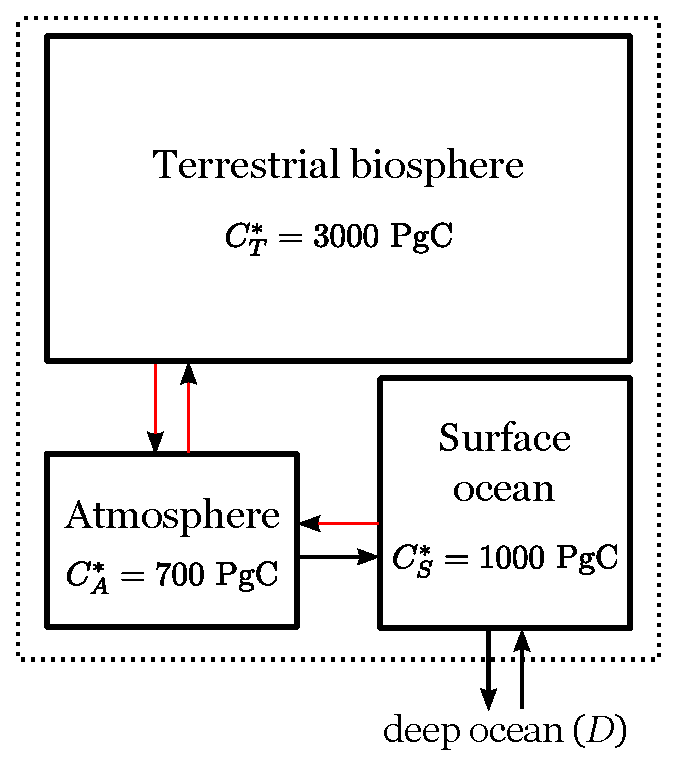
\includegraphics[height=0.7\textheight]{Figures/model_eq.pdf}
\end{figure}

}

\frame{ 
\frametitle{Equilibrium age densities}
  \begin{center} 
    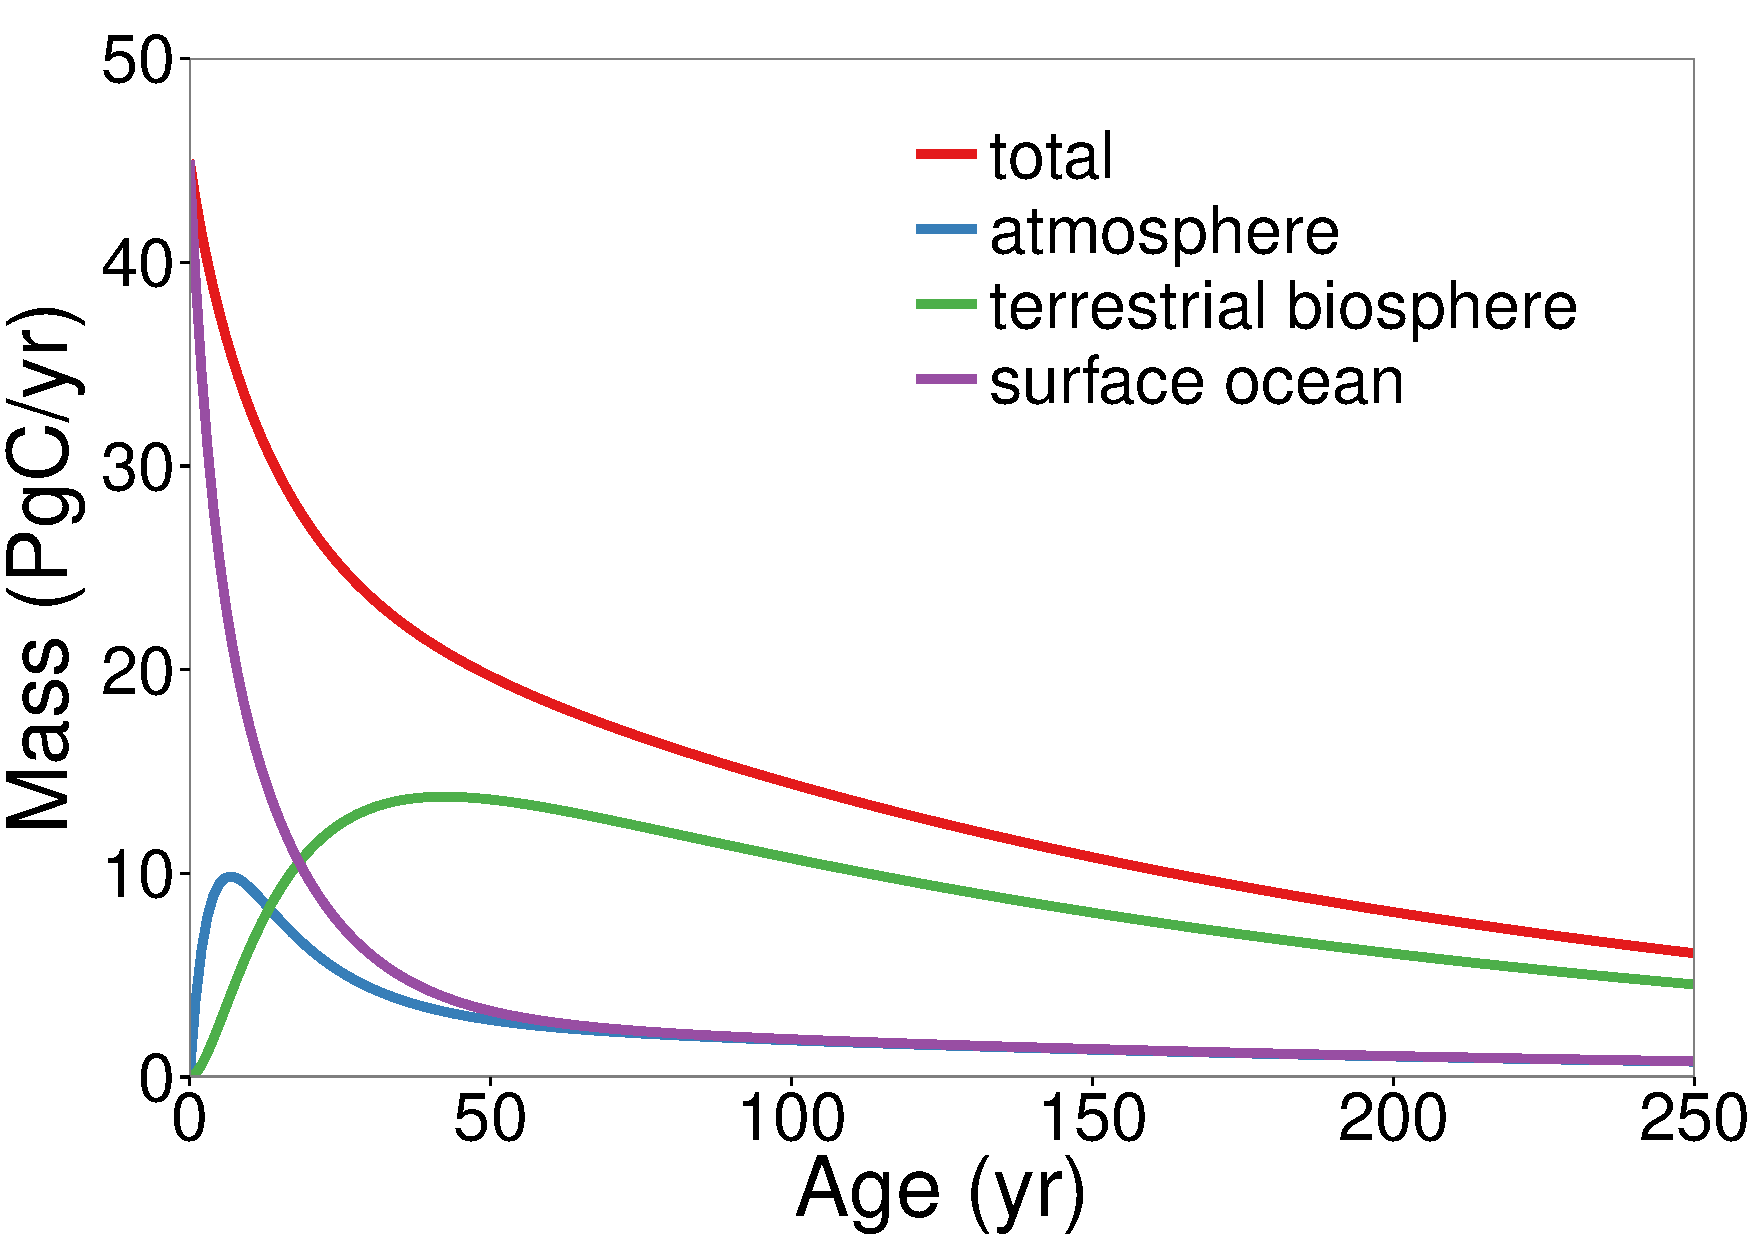
\includegraphics[width=0.9\textwidth]{Figures/equilibrium} 
  \end{center}
}


%%%%%%%%%%%%%%%%%%%%%%%%%%%%

\frame{ 
\frametitle{Linear \red{non}autonomous systems}
\uncover<-7>{
  \[
    \deriv{t}\,\vec{x}(t) = \tens{A}\red{(t)}\,\vec{x}(t)+\vec{u}\red{(t)}
  \]
}
\begin{itemize}
  \item<2-> \uncover<-7>{\textbf{general solution}}
  \[
    \uncover<-7>{
      \vec{x}(t) = \tens{\Phi}(t,0)\,\vec{x}^0 + \int_{0}^t \only<-6>{\tens{\Phi}(t,s)\,\vec{u}(s)}
    }
    \only<7->{\blue{\underbrace{\tens{\Phi}(t,s)\,\vec{\vec{u}(s)}}_{\text{mass with age }t-s\text{ at time }t}}}
    \uncover<-7>{\,ds}
  \]
  \only<9->{
    \[
      \qquad\qquad\qquad\Rightarrow\underbrace{\tens{\Phi}(t,t-a)\,\vec{u}(t-a)}_{\text{mass with age }a\text{ at time }t}
    \]
  }
\uncover<-7>{
  \item<3-> \textbf{special case of no time dependence}
  \[
    \vec{x}(t) = e^{t\,\tens{A}}\,\vec{x}^0 + \int_0^t \only<-5>{e^{(t-s)\,\tens{A}}\,\vec{u}} \only<6->{\blue{\underbrace{e^{(t-s)\,\tens{A}}\,\vec{u}}_{\text{mass with age }t-s\text{ at time }t}}}\,ds
  \]
  \item<4->[$\to$] compartmental age probability density
  \[
    \vec{f_a}(y) = \left(\tens{X}^\ast\right)^{-1}\,e^{y\,\tens{A}}\,\vec{u} \uncover<5->{\quad\Rightarrow\quad \blue{\text{mass with age }y:\; e^{y\,\tens{A}}\,\vec{u}}}
  \]
 }
\end{itemize}
}

\frame{
\frametitle{The state transition operator $\tens{\Phi}$}
\begin{itemize}
  \item solution to the matrix ordinary differential equation
  \[
    \deriv{t}\,\tens{\Phi}(t,s) = \tens{A}(t)\,\tens{\Phi}(t,s), \quad\text{initial condition }\tens{\Phi(s,s)} = \tens{I}
  \]
  
  \item<2-> time-independent system
  \[
    \tens{\Phi}(t,s) = e^{(t-s)\,\tens{A}}\quad\text{(matrix exponential)}
  \]

  \item<3-> one-dimensional system with $\tens{A} = -\lambda$,
  \[
    \Phi(t,s) = e^{-\lambda\,(t-s)}\quad\text{(exponential function)}
  \]
  
  \item<4->[$\to$] describes the time evolution of mass in the system
  \item<5->[$\to$] we can always obtain it (at least numerically)
\end{itemize}
}

\frame{ 
\frametitle{Splitting the system}
\begin{itemize}
  \item we split the system into two parts
	\begin{align*}
	 \parbox{3cm}{mass in the system at time $t$ with age $a$} &=
	 \begin{cases}
	   \uncover<3->{\parbox{3.7cm}{remainings from input at time $t-a$}}\uncover<2->{,  &a<t}\\
	   \\
	   \uncover<5->{\parbox{3.7cm}{remainings from initial content $\vec{x}^0$ with initial age $a-t$}}\uncover<2->{, \quad&a\geq t}\\
	 \end{cases}\\
	 \\
	 \uncover<4->{
	 &= \begin{cases}
	      \uncover<4->{\tens{\Phi}(t,t-a)\,\vec{u}(t-a),\quad  &a<t,}\\
	      \\
	      \uncover<6->{\tens{\Phi}(t,0)\,\vec{p}^0(a-t), \quad & a\geq t}
	    \end{cases}
	}
        \end{align*}
  \item<7-> $\vec{p}^0$ is a given age distribution of the initial content vector $\vec{x}^0$
\end{itemize}
}

\frame{
\frametitle{Transit time}
\begin{itemize}
  \item<1-> transit time := age of particles in the outflux
  \item[$\to$]<2-> transit time distribution is weighted average of 
  \begin{itemize}
    \item compartmental ages
    \item compartment contents
    \item outflow rates
  \end{itemize}
  \item[$\to$]<3-> mean, higher order moments, quantiles, \ldots
  \item[$\to$]<4-> \red{$\text{mean transit time} \neq \frac{\text{stock}}{\text{flux}}$}
\end{itemize}
}


% \frame{ 
% \frametitle{Additional information available}
% \begin{itemize}
%   \item total information about the age distribution at any time by (semi-)explicit formulas
%   \item[$\to$] possible \red{(semi-)analytic investigation of model's age properties}
%   \begin{itemize}
%     \item before: age distribution (if at all) available only through long-term simulation
%     \item no further investigation possible
%   \end{itemize}
%   
%   \item[$\to$] system of ordinary differential equations for time evolution of mean age \red{and higher order moments}
%   \begin{itemize}
%     \item before: ODE system only for the mean \citep{Rasmussen2016JMB}
%   \end{itemize}
% 
%   \item[$\to$] system of ordinary differential equations for time evolution of \red{age quantiles}
%   \begin{itemize}
%     \item median as unique $2$-quantile is a special case
%     \item before: no computation of quantiles possible at all
%   \end{itemize}
% \end{itemize}
% }

% \frame{
% \frametitle{Transit time}
% \begin{itemize}
%   \item \textbf{forward transit time} ($\FTT$)
%   \begin{itemize}
%     \item<2-> particle arrives at time $t_a$
%     \item<2-> $\FTT$ is the a random variable that describes the age $a$ the particle will have when it leaves the system at time $t_e=t_a+a$
%     \item<4-> \red{evaluated at arrival time}
%     \item<6-> hard to measure the future
%   \end{itemize}
%   \item \textbf{backward transit time} ($\BTT$)
%   \begin{itemize}
%     \item<3-> $\BTT$ is the a random variable that describes the age $a$ of the particle when it leaves the system at time $t_e$
%     \item<5-> \red{evaluated at exit time}
%     \item<7-> measurable with a labeling experiment
%   \end{itemize}
%   
%   \item<8-> knowledge of the state transition operator allows us to compute $\FTT$ and $\BTT$
%   \item<9-> $\BTT = \text{shifted }\FTT:\quad f_{\BTT}(a,\red{t_a}) = f_{\BTT}(a,\red{t_e})$
%   \item<10-> \red{$\text{mean transit time} \neq \frac{\text{stock}}{\text{flux}}$}
% \end{itemize}
% }


\frame{
\frametitle{\red{Non}linear nonautonomous systems}
  \[
    \deriv{t}\,\vec{x}(t) = \tens{A}(\red{\vec{x}(t)},t)\,\vec{x}(t)+\vec{u}(t)
  \]

\begin{itemize} 
  \item<1-> \textbf{linearization along a solution trajectory}
  \begin{itemize}
    \item<2-> solve this equation (numerically)
    \item<3-> plug the solution $\tilde{\vec{x}}$ into $\tens{A}$:
    \[
      \tilde{\tens{A}}(t):= \tens{A}(\tilde{\vec{x}}(t),t)
    \]
    \item[$\to$]<4-> \red{linear} nonautonomous system
    \[
      \deriv{t}\,\vec{x}(t) = \tilde{\tens{A}}(t)\,\vec{x}(t)+\vec{u}(t)
    \]
  \end{itemize}
\end{itemize}
}

\frame{
\frametitle{A global carbon cycle model}
\begin{figure}[htbp]
  \begin{minipage}{0.35\textwidth}
    \hspace{1cm}
    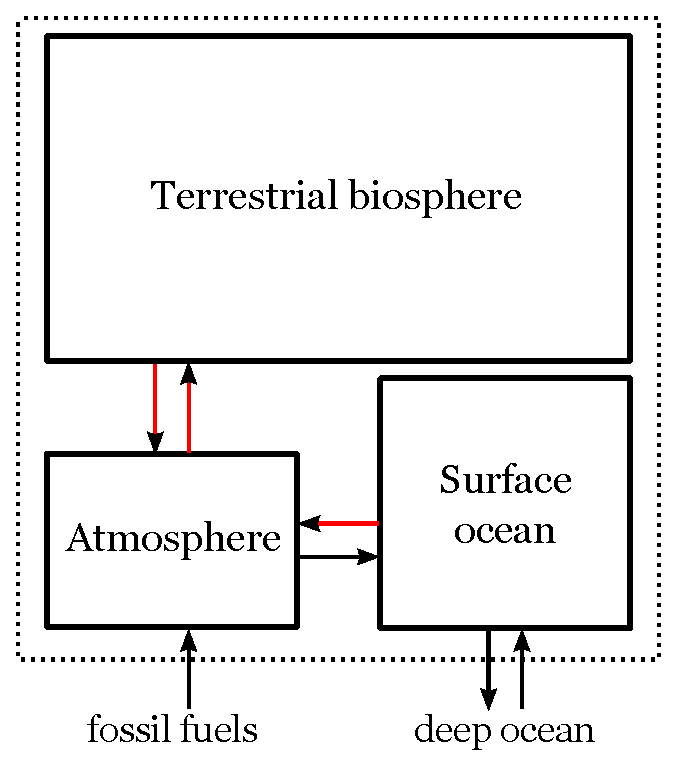
\includegraphics[width=\textwidth]{Figures/presentation/model}  
  \end{minipage}
  \hfill
  \uncover<2->{
  \begin{minipage}{0.52\textwidth}
    \center{\textbf{Equilibrium age densities in 1765}}\\
    %\vspace{0.5cm}
    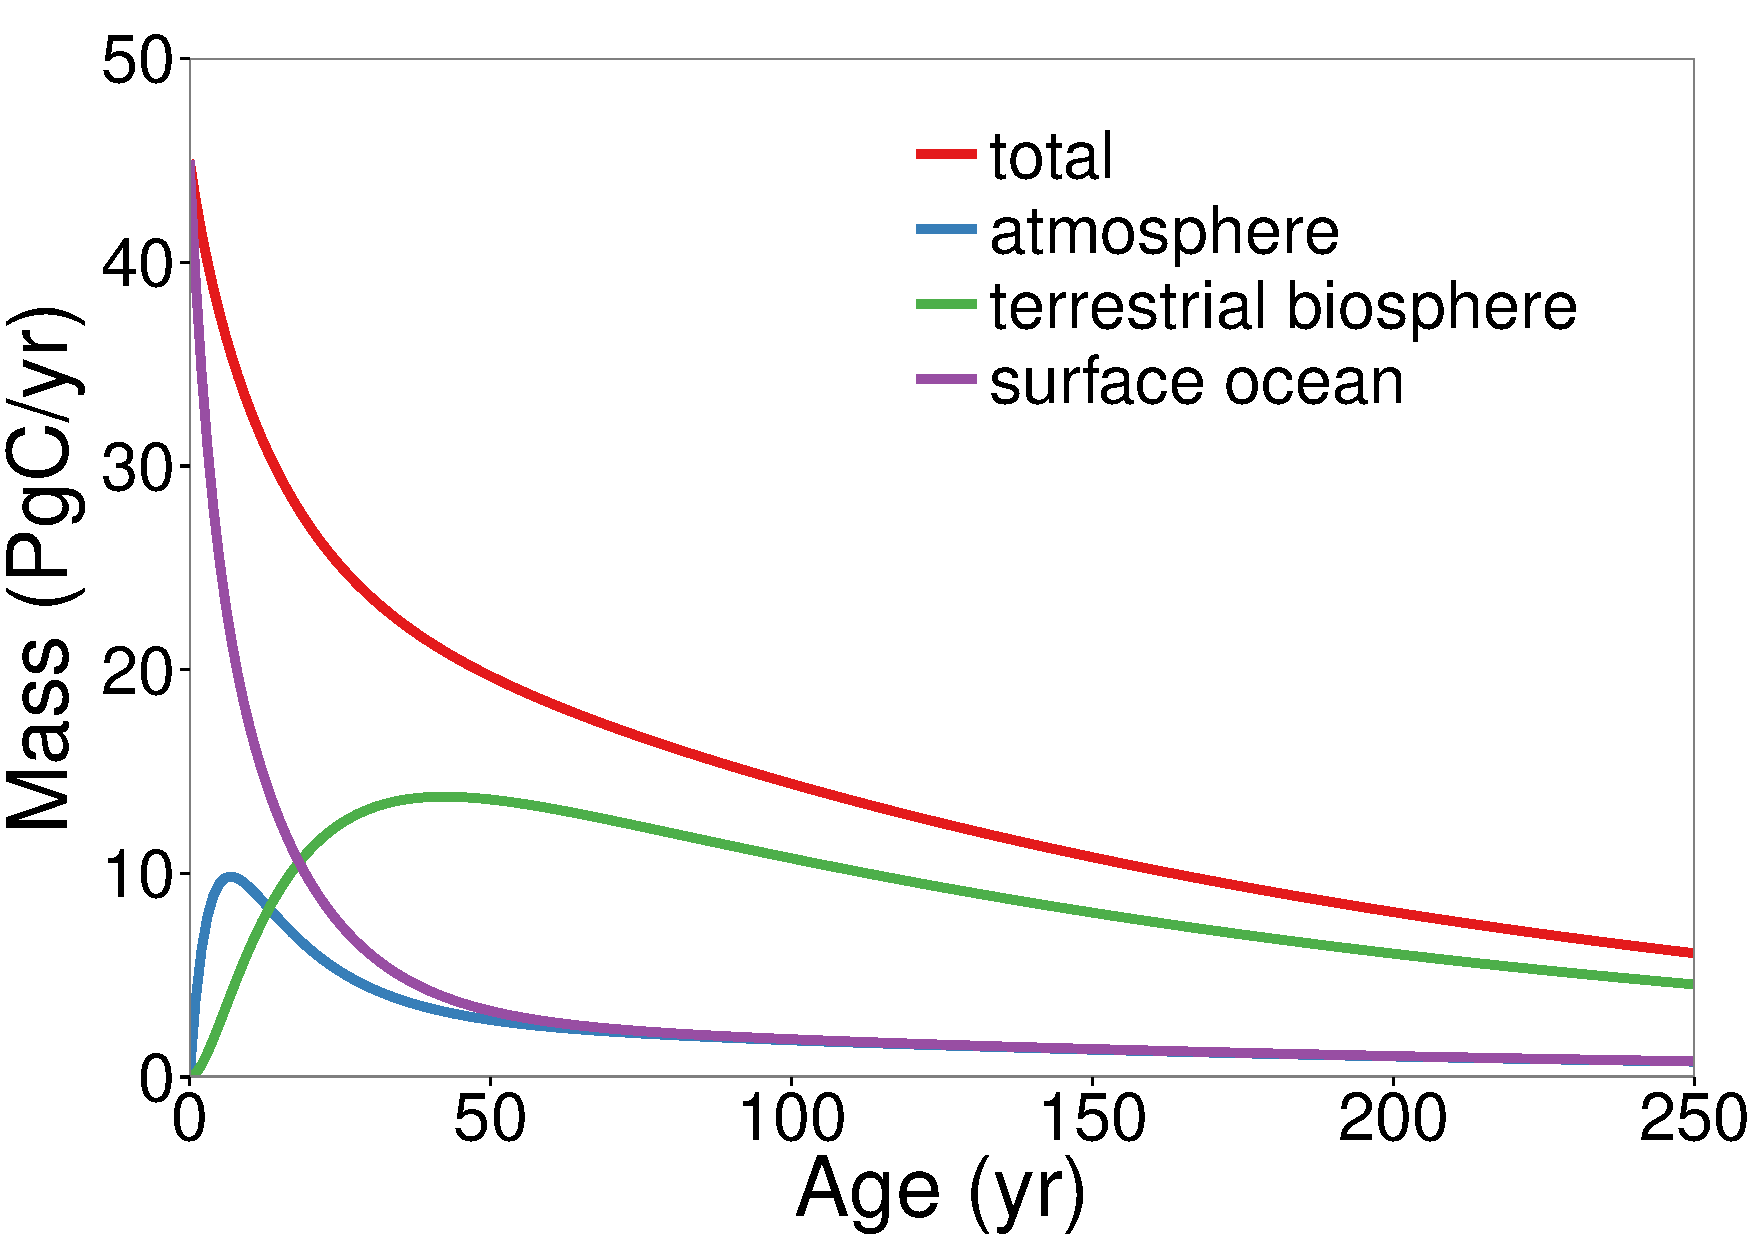
\includegraphics[width=0.7\textwidth]{Figures/equilibrium} 
    \uncover<3>{
    \center{\textbf{RCP8.5 scenario}}\\
    %\vspace{0.5cm}
      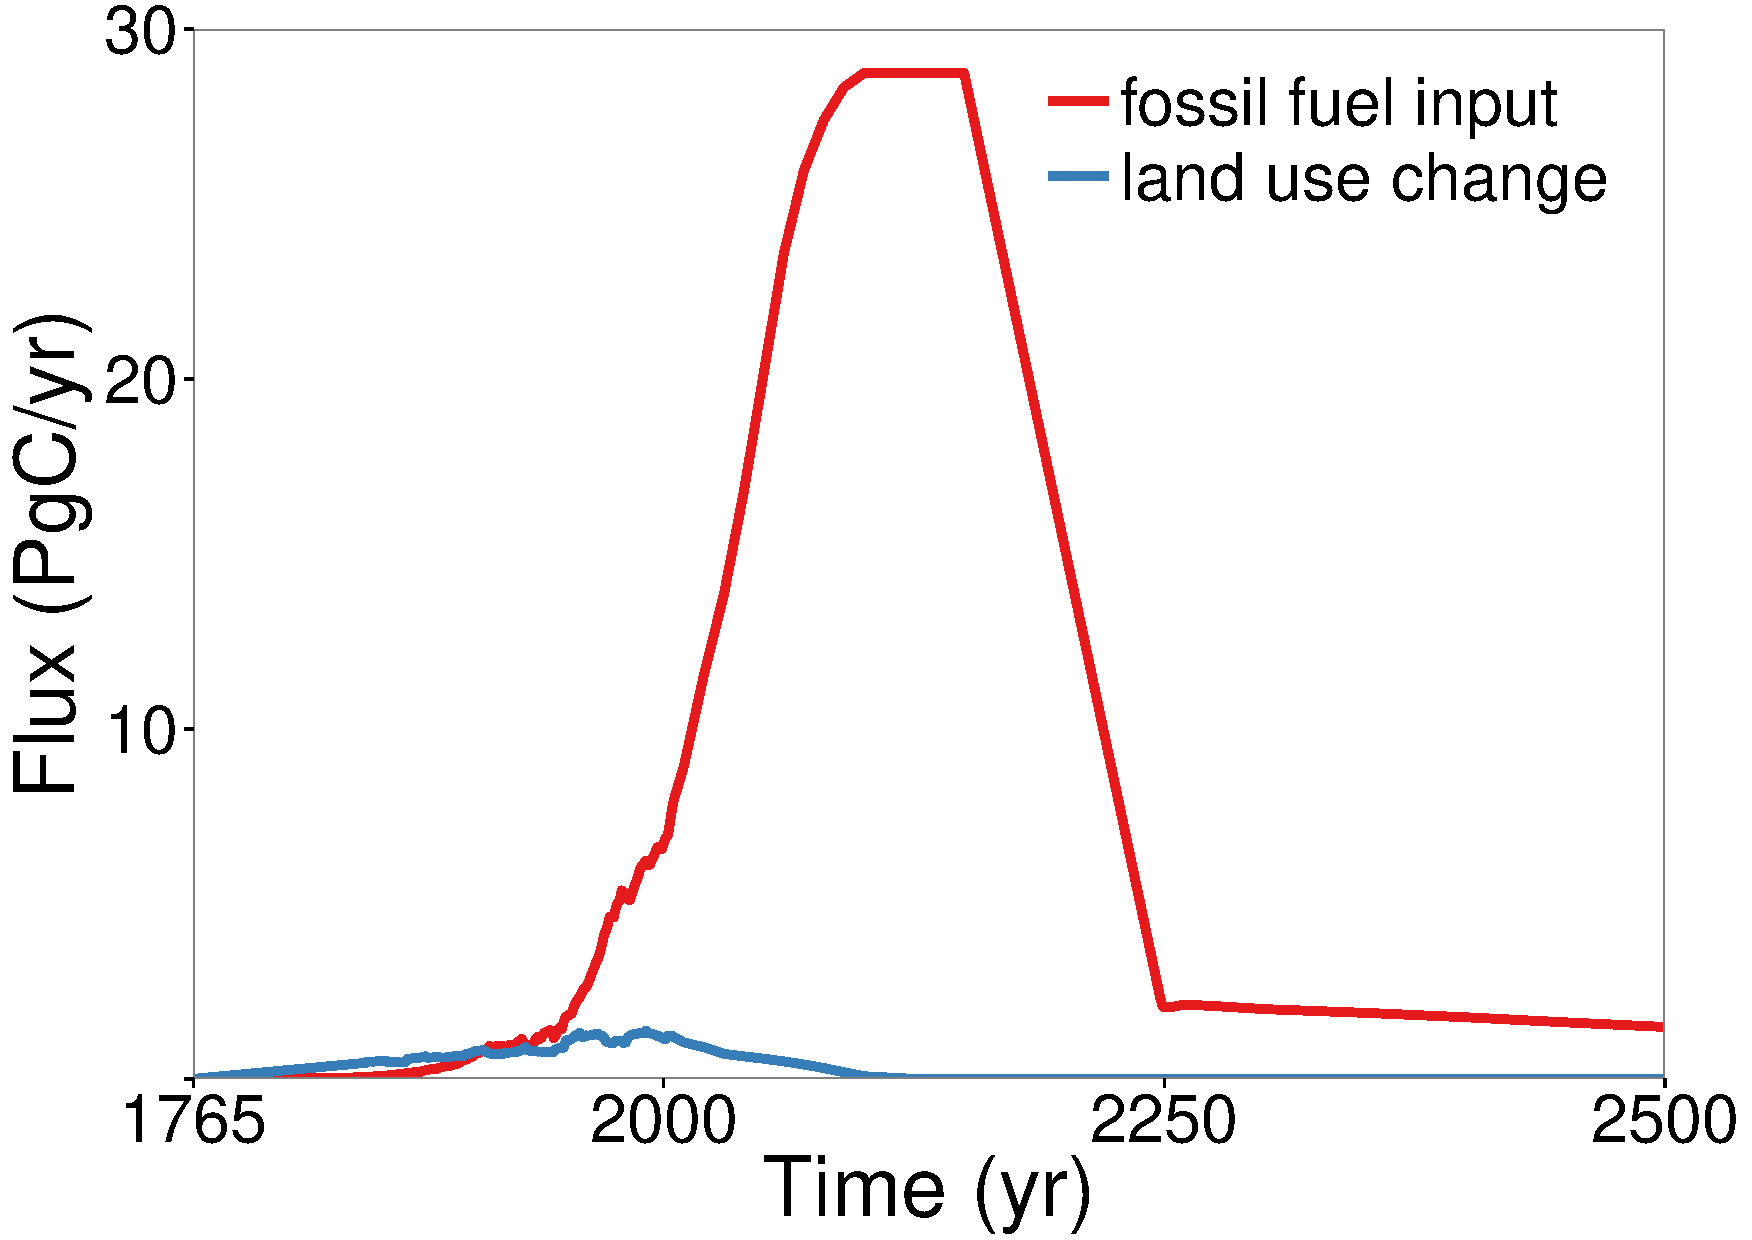
\includegraphics[width=0.7\textwidth]{Figures/perturb}
    }
  \end{minipage}  
  }
\end{figure} 
}
 
\frame{
\frametitle{Time-dependent carbon contents}
  \begin{center}
    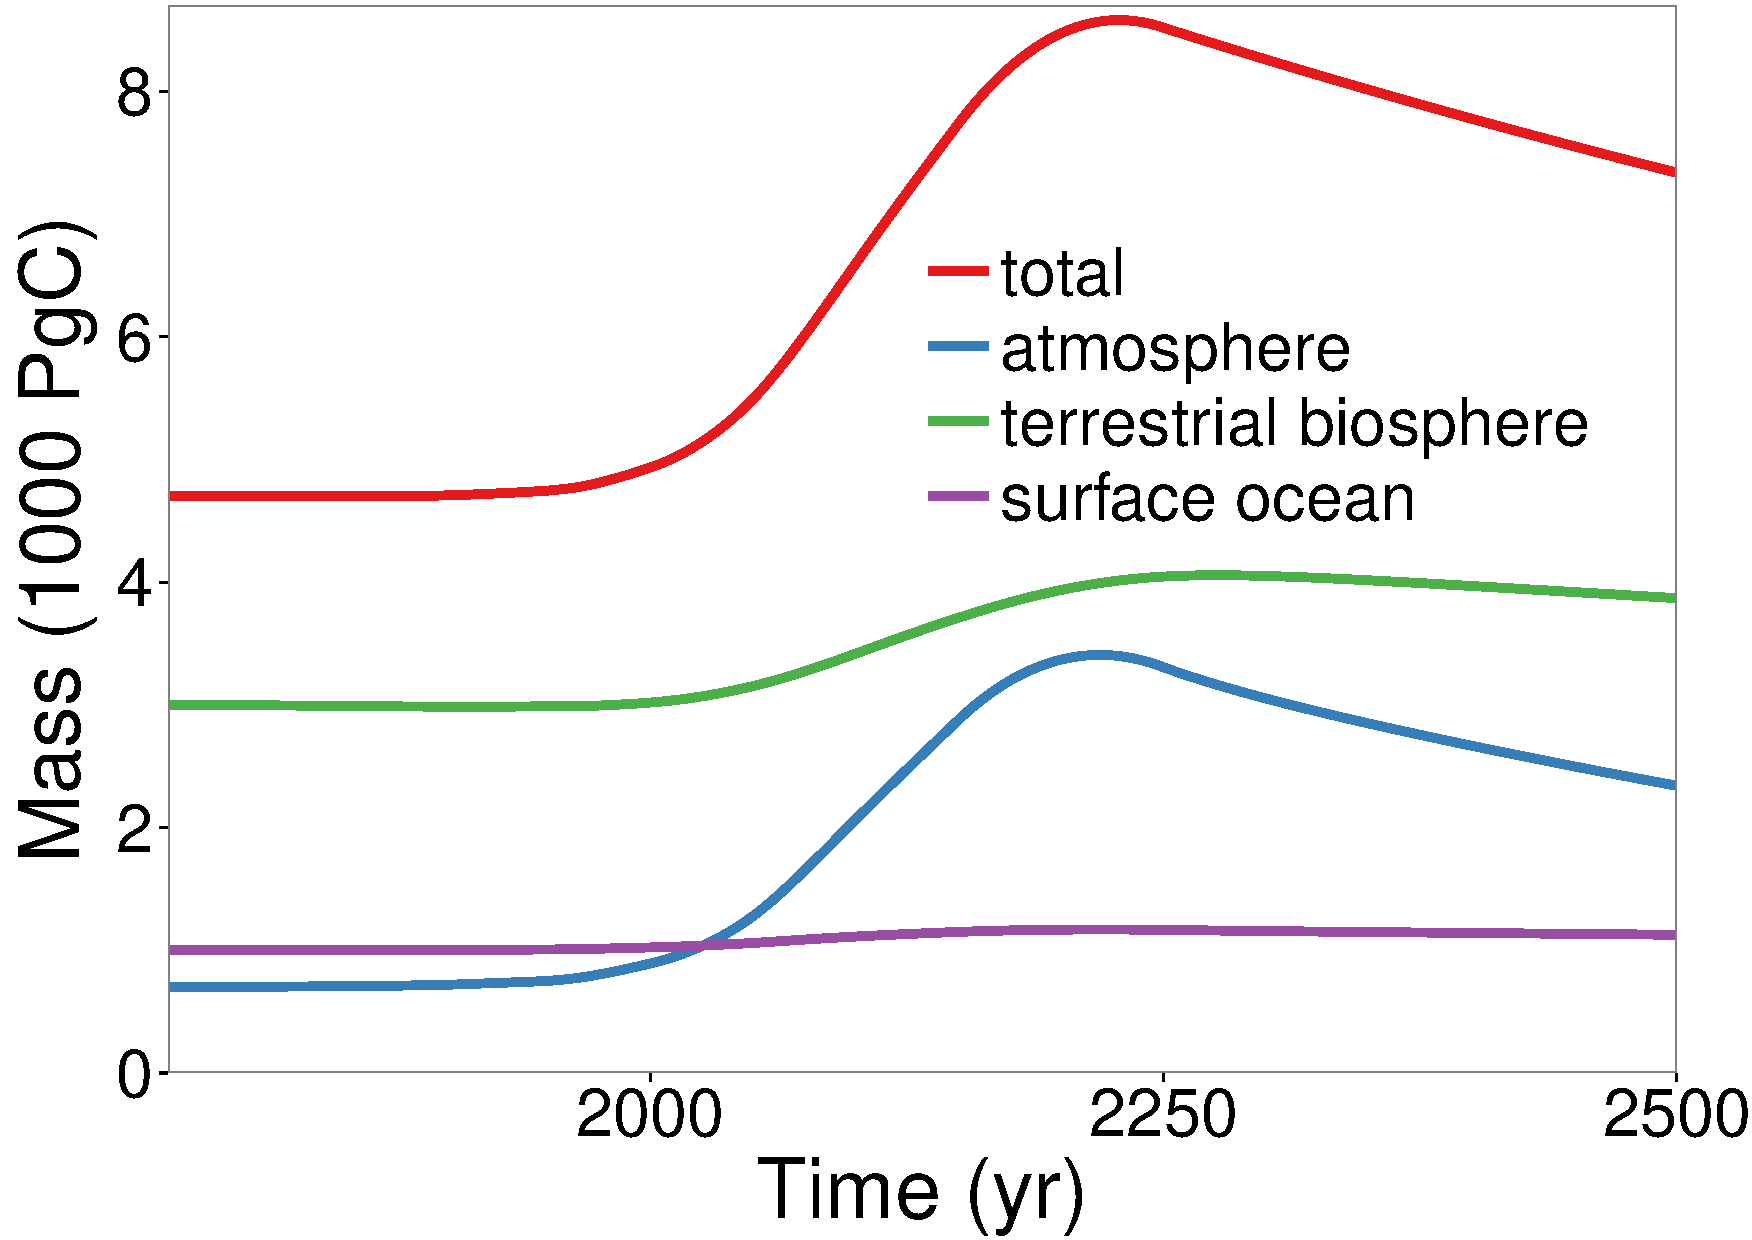
\includegraphics[height=0.8\textheight]{Figures/sol}
  \end{center}
}

\frame{
\frametitle{Questions of high scientific and societal interest}
  \begin{itemize}
    \item[1.] \textbf{Origin of current effects:} How old is the current atmospheric burden?
  \end{itemize}

  \uncover<2->{
    \begin{center}
      \vspace{-0.5cm}
      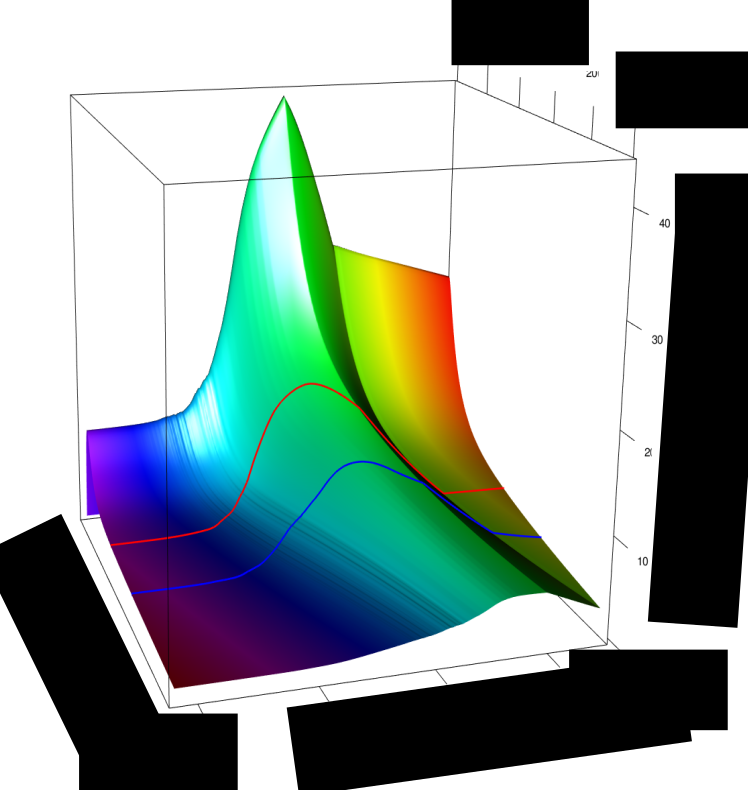
\includegraphics[height=0.8\textheight]{Figures/atmosphere}
    \end{center}
  }
}

\frame{
\frametitle{Questions of high scientific and societal interest}
  \begin{itemize}
    \item[2.] \textbf{Future commitment:} If we allow a pulse of $1$ PgC to be emitted today, how long will a significant fraction of this excess remain in the system?
  \end{itemize}

  \uncover<2->{
    \begin{center}
      \vspace{-0.15cm}
      \includegraphics<-2>[height=0.7\textheight]{Figures/ftt1}
      \includegraphics<3>[height=0.7\textheight]{Figures/ftt2}
      \includegraphics<4>[height=0.7\textheight]{Figures/ftt3}
      \includegraphics<5>[height=0.7\textheight]{Figures/ftt4}
      \includegraphics<6>[height=0.7\textheight]{Figures/ftt5}
    \end{center}
  }
}


% \frame{
% \frametitle{Questions of high scientific and societal interest}
%   \begin{itemize}
%     \item[3.] How old is the carbon that leaves the system toward the deep ocean?
%   \end{itemize}
% 
%   \uncover<2->{
%     \begin{center}
%       \vspace{-0.15cm}
%       \includegraphics<-2>[height=0.7\textheight]{Figures/btt1} 
%       \includegraphics<3>[height=0.7\textheight]{Figures/btt2} 
%     \end{center}
%   }
% }

%%%%%%%%%%%%%%%%%%%%%%%%
\frame{ 
\frametitle{Summary}
\begin{itemize}
  \item <1-> \textbf{carbon cycle models $\leftrightarrow$ stochastic processes}
  \begin{itemize}
    \item linear autonomous compartmental models $\leftrightarrow$ continuous-time Markov chains
  \end{itemize}
  \item <2-> \textbf{general, simple, explicit formulas}
  \begin{itemize}
    \item transit time, system age, compartment age densities
    \item[$\to$] \red{no long-time simulation needed}
    \item[$\to$] \red{no complicated treatment of special cases}
  \end{itemize}
  \item <3-> \textbf{stochastic toolbox}
  \begin{itemize}
    \item deviations from mean behavior
    \item higher order moments, quantiles
    \item confidence intervals consideration possible
  \end{itemize}
  \item< 4-> \textbf{two Python packages}
  \begin{itemize}
    \item (symbolic) computation of age and transit time properties for autonomous systems in steady state
    \begin{itemize}
      \item \url{http://github.com/goujou/LAPM}
    \end{itemize}
    \item (numerical) computation of age and transit time properties for nonlinear nonautonomous systems
  \end{itemize}
\end{itemize}
}

%%%%%%%%%%%%%%%%%%%%%%%%

\frame{
\begin{center}\vspace{-1cm}
  \only<1>{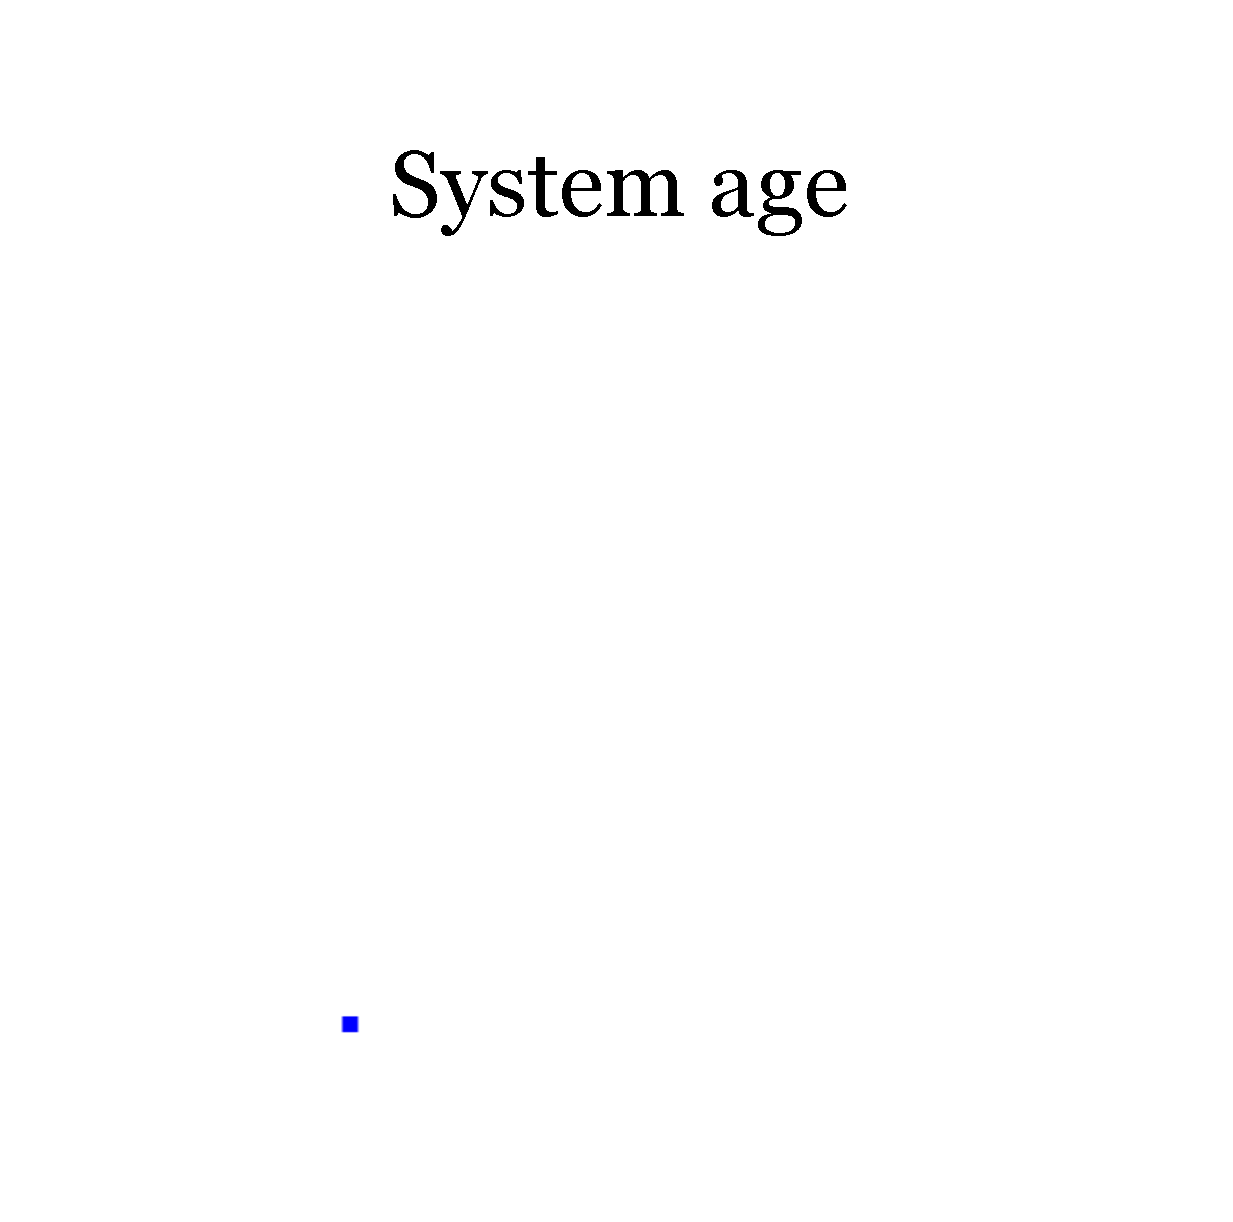
\includegraphics[scale=0.5]{Figures/presentation/1.pdf}}
  \only<2>{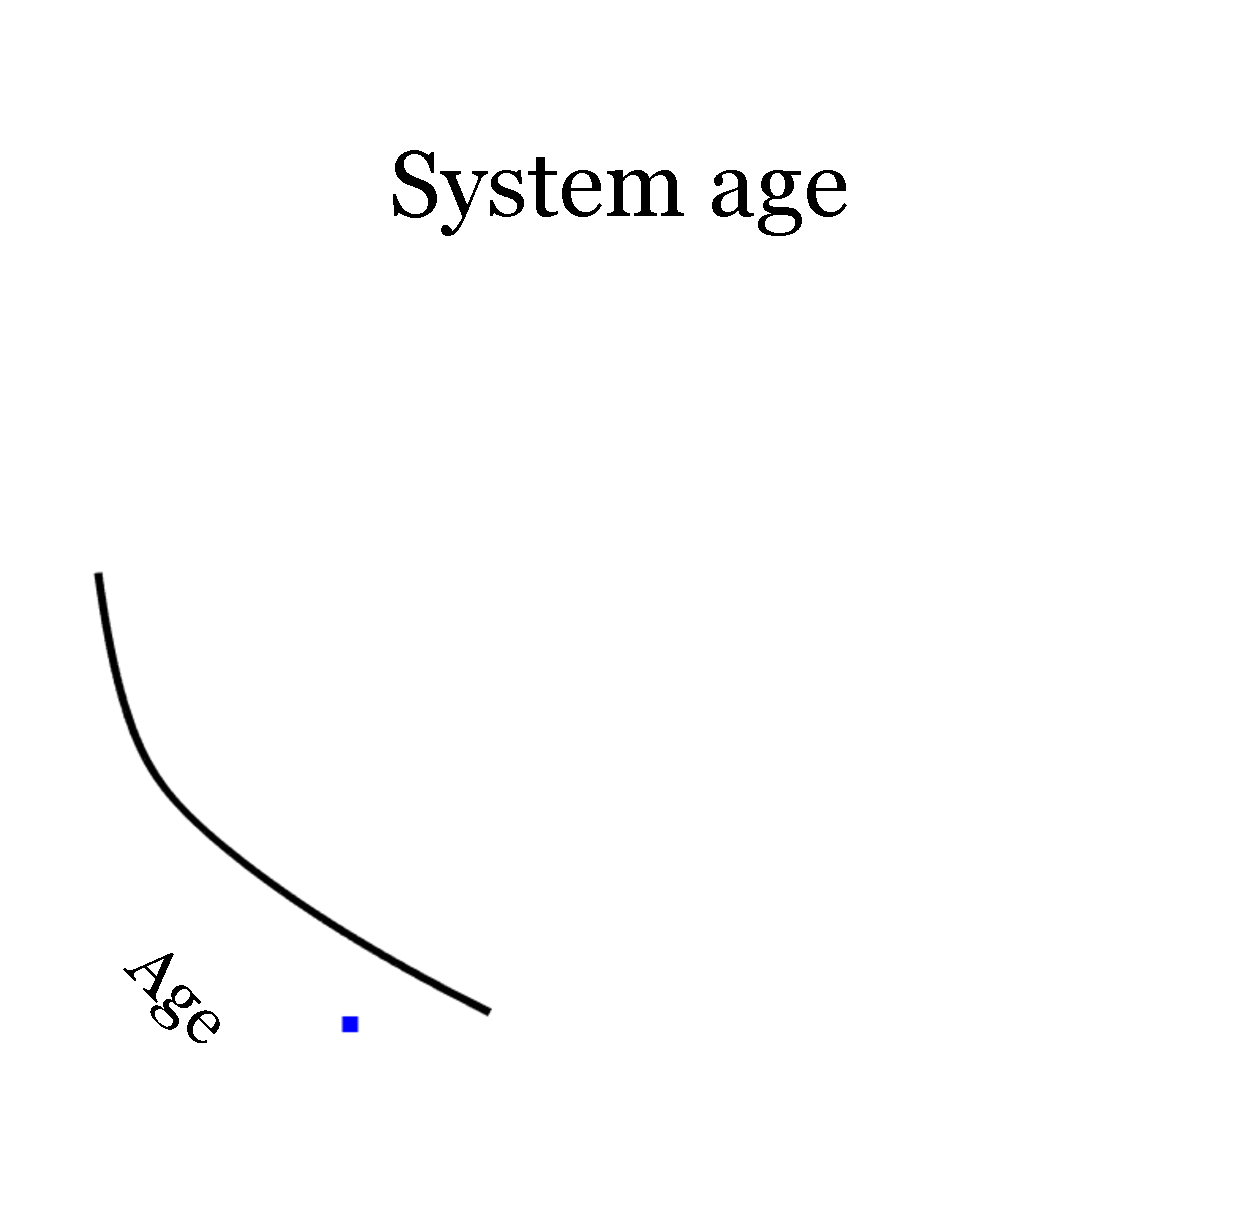
\includegraphics[scale=0.5]{Figures/presentation/2.pdf}}
  \only<3>{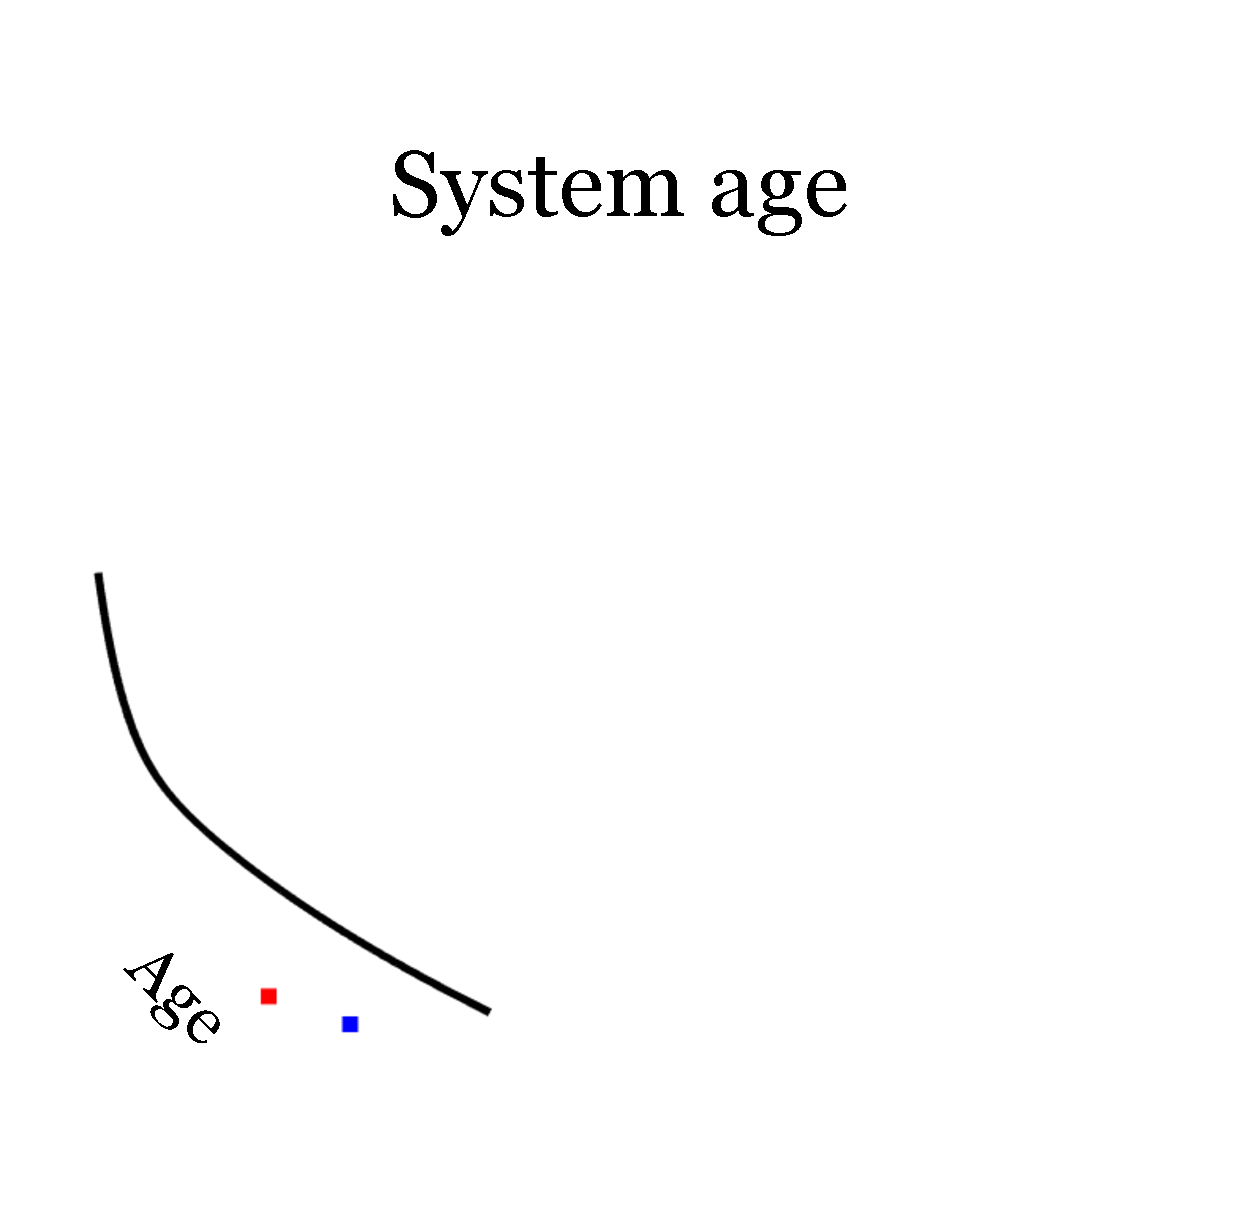
\includegraphics[scale=0.5]{Figures/presentation/3.pdf}}
  \only<4>{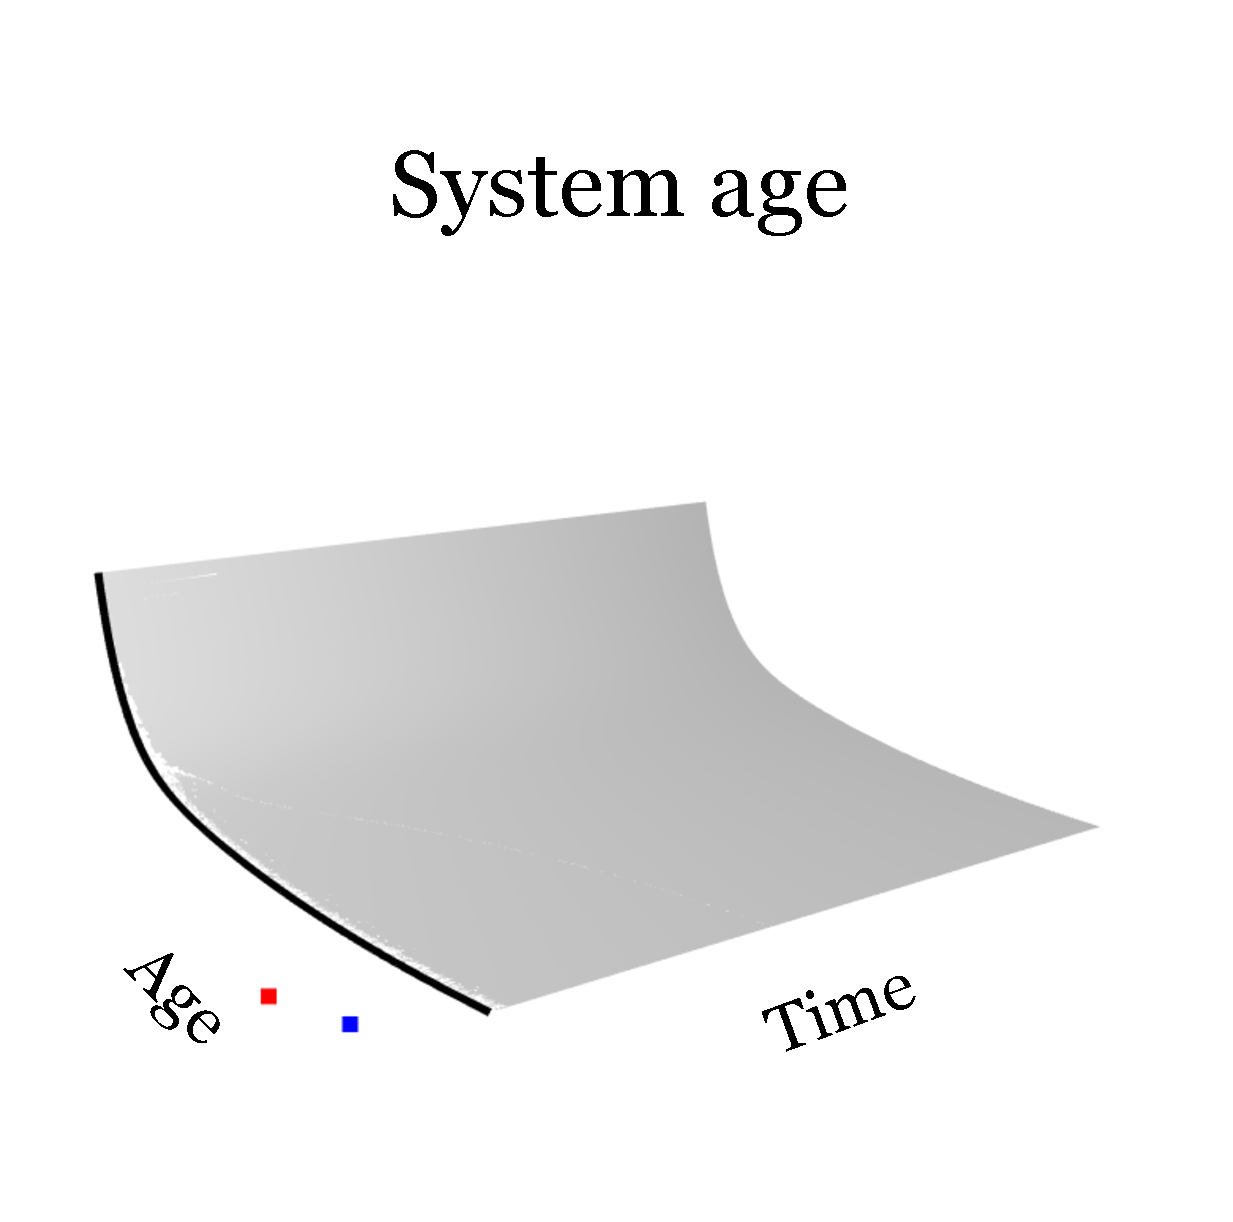
\includegraphics[scale=0.5]{Figures/presentation/4.pdf}}
  \only<5>{\includegraphics[scale=0.5]{Figures/presentation/5.pdf}}
  \only<6>{\includegraphics[scale=0.5]{Figures/presentation/6.pdf}}
  \only<7>{\includegraphics[scale=0.5]{Figures/presentation/7.pdf}}
  \only<8>{\includegraphics[scale=0.5]{Figures/presentation/8.pdf}}
  \only<9>{\vspace{0.4cm}\includegraphics[scale=0.45]{Figures/presentation/total.pdf}}
  \only<10>{\vspace{0.4cm}\includegraphics[scale=0.45]{Figures/presentation/final.pdf}}
\end{center}
}

%%%%%%%%%%%%%%%%%%%%%%%%


\frame{
\frametitle{Thanks}

\begin{center}
  \bf{Funding}\\
  \vspace{1cm}
  \includegraphics[scale=0.07]{EmmyNoether} \hspace{5em}
  \includegraphics[scale=0.3]{Minerva}
\end{center}
}
%\begin{frame}
% [fragile]
%\frametitle{Example Model}
%\makebox[0pt][l]{
%  \includegraphics<1>[width=0.9\textwidth]{LasagaModel.pdf}
%  \includegraphics<2,3,4,5,6,7,8>[width=0.9\textwidth]{LasagaModelTransp.pdf}
%  }
%\raisebox{4cm}{
%\begin{minipage}{10cm}
%   \begin{itemize}
%      \item<2,3,4,5,6,7,8>
%	 We want to observe the behavior of arbitrary complex reservoir systems 
%	 under all imaginable conditions,which e.g. means:\\
%	 %\begin{itemize}
%	    \item<3,4,5,6,7,8>
%	       time dependent transfer rates.
%	    \item<4,5,6,7,8>
%	       time dependent inputs
%	    \item <5,6,7,8>
%	       non linear behavior
%	    \item<6,7,8>
%	       arbitrary perturbations (non steady states)
%	    \item<7,8>
%	       closed and open systems
%	    \item<8>
%	       reservoirs with nested reservoirs
%	 %\end{itemize}
%   \end{itemize}
%\end{minipage}
%}
%  \note{
%  We want to observe the behavior of arbitrary complex reservoir systems 
%  under all imaginable conditions. \\
%  To raise your interest we have chosen an example of an old global Carbon cycle model, that 
%  has some of the features we are interested in.}
%\end{frame}
%%%%%%%%%%%%%%%%%%%%%%%%%%%%%%%%%%%%%%%%%%%%%%%%%%%%%%%%%%%%%%%%%%%%%%%%%%%%%%%%%%%%%%%%%%%%%%%%%%%%%
%\begin{frame}
% [fragile]
%\frametitle{inappropriateness of previously proposed analytical solutions}
%\begin{itemize}
%      \pause
%      \item
%	 Only available for special cases 
%      \pause
%      \item
%	 involve a lot of assumptions that can be confusing sometimes, e.g.:
%      \pause
%      \begin{itemize}
%	    \item
%	    steady states, 
%      \pause
%	    \item
%	    time invariant systems
%      \pause
%	    \item
%	    linear systems 
%      \pause
%	    \item
%	    impulsive or constant inputs 
%      \pause
%      \end{itemize}
%      \pause
%      \item
%	 assumptions sometimes hard to recognize 
%	 \\
%      \pause
%	 $\rightarrow$ misleading into wrong generalizations
%	 \\
%      \pause
%	 $\rightarrow$ motivation for a numerical counterpart 
%	 where all the assumptions (if any) should be 
%	 {\color{red} intuitive and obvious.}
%\end{itemize}
%\end{frame}
%%%%%%%%%%%%%%%%%%%%%%%%%%%%%%%%%%%%%%%%%%%%%%%%%%%%%%%%%%%%%%%%%%%%%%%%%%%%%%%%%%%%%%%%%%%%%%%%%%%%%%
%\section{Our proposed solution}
%\subsection{Definitions}
%
%%%%%%%%%%%%%%%%%%%%%%%%%%%%%%%%%%%%%%%%%%%%%%%%%%%%%%%%%%%%%%%%%%%%%%%%%%%%%%%%%%%%%%%%%%%%%%%%%%%%%%
%\begin{frame}
% [fragile]
%\frametitle{Requirements for definitions}
%definitions should be:
%\begin{enumerate}
%      \pause
%   \item as generally applicable as possible\\
%      $\rightarrow$ observable even in the real world
%      \pause
%   \item easy to check
%      \pause
%   \item suitable for computer simulations \\
%      \pause
%      $\rightarrow$ based on a definite time scale with
%      \begin{enumerate}
%	 \item definite start
%	 \item definite end \\
%      \pause
%	 $\rightarrow$ no $\infty$
%      \end{enumerate}
%\end{enumerate}
%\note{
%Assume that we want to run a particle simulation, that we want to ``observe'' So all features used should be observable in the real world too.
%To formulate the problem in a numerical way we need to define the basic concepts precisely and in a way that a computer would understand. This means that we should avoid infinities.
%While the definitions are clear in some cases, there are subtle differences in details that may change the interpretations considerably.}
%\end{frame}
%%%%%%%%%%%%%%%%%%%%%%%%%%%%%%%%%%%%%%%%%%%%%%%%%%%%%%%%%%%%%%%%%%%%%%%%%%%%%%%%%%%%%%%%%%%%%%%%%%%%%%%
%\begin{frame}
%\frametitle{The general concept of a reservoir}
%  %\includegraphics[height=0.8\textheight]{Reservoir.pdf}
%  \includegraphics<1>[height=0.5\textheight]{Reservoir.pdf}
%  %\includegraphics<2>[height=0.5\textheight]{Reservoir_People.pdf}
%  \includegraphics<3,4>[height=0.5\textheight]{ReservoirNested.pdf} 
%  \begin{enumerate}
%\item <1,2,3,4> 
%   In and out ``flows'' must be unambiguously  defined \\
%\item <2,3,4> 
%   ``Flows'' do not necessarily involve ``movement'' \\
%     In and out flow ``channels'' do not always have to be defined physically or spatially 
%\item <3,4> 
%   reservoirs can have arbitrary complex subsctructures
%\item <4> 
%   reservoirs can be mixed or not
%\end{enumerate}
%\note<1>{Imagine a reservoir of particles with an input and an output channel. 
%Particles will enter the system through some input channel, will stay there for a while and eventually leave the system through an output stream. 
%Here Only the dark blue particles are ``in'' the reservoir. 
%}
%\note<2>{
%Although the concept of a reservoir is usually intuitively attached to some kind of a pool with fluid moving trough it 
%the idea is more general. 
%
%An example that shows how generally this idea can be applied is the human population of the world.
%A particle here refers to a human being that is born, lives and dies.
%
%The inflow and outflow boundaries are not spatially defined in this case 
%}
%
%\end{frame}
%%%%%%%%%%%%%%%%%%%%%%%%%%%%%%%%%%%%%%%%%%%%%%%%%%%%%%%%%%%%%%%%%%%%%%%%%%%%%%%%%%%%%%%%%%%%%%%%%%%%%%
%\begin{frame}
%      \pause
%\begin{enumerate}
%   \item describe the rate of change for the stuff inside the system in the form inputrate - outputrate
%      which is possible for all reservoir systems:
%      $\dot{C}=F(C,t)=I(C,t)-O(C,t)$
%      \pause
%   \item solve the possibly nonlinear system (compute $C(t)$)
%      \pause
%   \item use the solution to transform it to a linear uncoupled system with {\color{red} exactly } the same solution
%      \pause
%   \item for every $t$ and every $a:0<a<t$ compute $\psi(a,t)$
%      \pause
%   \item for every $t$ 
%   	 compute the expected value of $a$ by integrating over the product:
%	 \[ 
%	 E(t)=\int_0^t \psi(a,t) \;a \; da
%	 \]
%\end{enumerate}
%\end{frame}
%%%%%%%%%%%%%%%%%%%%%%%%%%%%%%%%%%%%%%%%%%%%%%%%%%%%%%%%%%%%%%%%%%%%%%%%%%%%%%%%%%%%%%%%%%%%%%%%%%%%%%
%\begin{frame}
% [fragile]
%\frametitle{Transforming the system I}
%  inject the solution into the operator
%      \begin{eqnarray*}
%	 \dot{\vec{F}}	&=&\dot{\vec{C}}(\vec{C},t)\\
%	 &=&
%	 \left(
%	 \begin{array}{c}
%	    \dot{F}_1(C_1,\hdots ,C_n,t)\\
%	    \vdots \\
%	    \dot{F}_n(C_1,\hdots ,C_n,t)
%	 \end{array}
%	 \right)
%	 \\
%	 &=&
%	 \left(
%	 \begin{array}{c}
%	    \dot{I}_1(C_1,\hdots ,C_n,t)\\
%	    \vdots \\
%	    \dot{I}_n(C_1,\hdots ,C_n,t)
%	 \end{array}
%	 \right)
%	 +
%	 \left(
%	 \begin{array}{c}
%	    \dot{O}_1(C_1,\hdots ,C_n,t)\\
%	    \vdots \\
%	    \dot{O}_n(C_1,\hdots ,C_n,t)
%	 \end{array}
%	 \right)
%      \end{eqnarray*}
%\end{frame}
%%%%%%%%%%%%%%%%%%%%%%%%%%%%%%%%%%%%%%%%%%%%%%%%%%%%%%%%%%%%%%%%%%%%%%%%%%%%%%%%%%%%%%%%%%%%%%%%%%%%%%
%\begin{frame}
% [fragile]
%\frametitle{Transforming the system II}
%  For every component $F_i$ do:    
%      \begin{eqnarray*}
%	 \dot{F}_i(t) &=&\frac{I_i(C_1(t),\hdots ,C_n(t),t)}{C_i(t)}C_i(t)-\frac{O_i(C_1(t),\hdots ,C_n(t),t)}{C_i(t)}C_i(t)\\
%	 &=&I_{i_{lin}}(t)C_i(t)-O_{i_{lin}}(t)C_i(t)\\
%	 &=&F_{i_{lin}}(t)C_i(t)
%      \end{eqnarray*}
%  Now the equations are uncoupled and linear.    
%%      for all times ${\color{red}t}$ for which the result is sought compute $\bar{a}({\color{red}t})$ as follows: (the next slide has to be evaluated many times)
%\end{frame}
%%%%%%%%%%%%%%%%%%%%%%%%%%%%%%%%%%%%%%%%%%%%%%%%%%%%%%%%%%%%%%%%%%%%%%%%%%%%%%%%%%%%%%%%%%%%%%%%%%%%%%%
%\begin{frame}
% [fragile]
%\frametitle{Accumulating previous inputs}
%\begin{knitrout}\footnotesize
%\definecolor{shadecolor}{rgb}{0.969, 0.969, 0.969}\color{fgcolor}
%
%{\centering \includegraphics[width=.7\linewidth]{figure/beamer-O12-1} 
%
%}
%
%
%
%\end{knitrout}
%\end{frame}
%%%%%%%%%%%%%%%%%%%%%%%%%%%%%%%%%%%%%%%%%%%%%%%%%%%%%%%%%%%%%%%%%%%%%%%%%%%%%%%%%%%%%%%%%%%%%%%%%%%%%%%
%\begin{frame}
% [fragile]
% \frametitle{Compute $\psi( {\color{green}a}, {\color{red}t})$ }
% for every possible age $0<{\color{green}a}<{\color{red}t}$ (nested loop) compute the probability density
% $\psi(
% {\color{green}a},
% {\color{red}t}
% )$ 
% as follows:
%   	 \begin{enumerate}
%      \pause
%   	    \item
%   	       collect all inputs that have occurred since $t-a$   
%      \pause
%   	    \item 
%	       predict their time development (vanishing) under no input conditions (solve for $O_{lin}$)
%      \pause
%   	    \item 
%   	       integrate over all those partly vanished inputs to find out what is left of
%   	       the lot
%      \pause
%   	    \item 
%   	       divide by the amount of stuff present in the reservoir right now to get the probability for a particle 
%   	       to have age less than a and be still around.
%      \pause
%	    \item
%	       compute the derivative with respect to $a$ 
%   	 \end{enumerate}
%\end{frame}
%
%%%%%%%%%%%%%%%%%%%%%%%%%%%%%%%%%%%%%%%%%%%%%%%%%%%%%%%%%%%%%%%%%%%%%%%%%%%%%%%%%%%%%%%%%%%%%%%%%%%%%%
%\subsection{Comparison to standard theory}
%%%%%%%%%%%%%%%%%%%%%%%%%%%%%%%%%%%%%%%%%%%%%%%%%%%%%%%%%%%%%%%%%%%%%%%%%%%%%%%%%%%%%%%%%%%%%%%%%%%%%%
%\begin{frame}
% [fragile]
%\frametitle{Conceptual example}
%\begin{itemize}
%   \item Input(rate): impulsive only at the start $\dot{I}=C_0\delta(0)$
%   \item Output(rate): $\dot{O}(C,t)=-k C(t)$ 
%   \item wanted: $C(t),\phi(t),\psi(t),\bar{t_r},\bar{a}$
%      \pause
%   \item solution:
%   \begin{itemize}
%      \pause
%      \item 
%	 $C(t)=C_0 e^{-k t}$   
%\begin{knitrout}\footnotesize
%\definecolor{shadecolor}{rgb}{0.969, 0.969, 0.969}\color{fgcolor}
%
%{\centering \includegraphics[width=.6\linewidth]{figure/beamer-O-1} 
%
%}
%
%
%
%\end{knitrout}
%      \end{itemize}
%   \end{itemize}
%\end{frame}
%%%%%%%%%%%%%%%%%%%%%%%%%%%%%%%%%%%%%%%%%%%%%%%%%%%%%%%%%%%%%%%%%%%%%%%%%%%%%%%%%%%%%%%%%%%%%%%%%%%%%%
%\begin{frame}
% [fragile]
%\frametitle{Intuitive solution for the example}
%   \includegraphics<1>[width=\textwidth]{MeanAgeImpuls.pdf}
%\end{frame}
%%%%%%%%%%%%%%%%%%%%%%%%%%%%%%%%%%%%%%%%%%%%%%%%%%%%%%%%%%%%%%%%%%%%%%%%%%%%%%%%%%%%%%%%%%%%%%%%%%%%%%%
%\begin{frame}
%[fragile]
%\frametitle{Theory for the example}
%      Manzoni,Katul,Porporato 2009:\\
%      ``for any linear systems  the transit time
%      distribution is the output flow resulting from an impulsive
%      unitary input.''
%   \begin{eqnarray*}
%      O(t)&=&\int_{0}^{\infty} \psi(T)I(t-T)dT
%	 \\
%	 &=&\psi(t) \text{ for } I=\delta(t-T)
%	 \\
%	 &=& e^{-kt} 
%   \end{eqnarray*}
%      \pause
%   Additionally we have:\\
%      $\phi(a)=\psi(a)=e^{-k a},\bar{t_r}=\bar{a}=\frac{1}{k}$
%   \\
%   Questions:
%	 \pause
%   \begin{itemize}
%      \item Where does the $\infty$ come from?
%	 \pause
%      \item is $\phi(a)=\psi(a)=e^{-k a}$ a probability density if we start the whole thing at some 
%	 definite time and not infinitely long ago? \\
%	 (does it integrate to $1$ ?)
%	 \pause
%      \item Are the above densities valid for arbitrary inputrates  $I(t)$ 
%	 \\
%	 (as functions of time.) 
%	 \pause
%	 \note{may be forever}
%   \end{itemize}
%\end{frame}
%%%%%%%%%%%%%%%%%%%%%%%%%%%%%%%%%%%%%%%%%%%%%%%%%%%%%%%%%%%%%%%%%%%%%%%%%%%%%%%%%%%%%%%%%%%%%%%%%%%%%%%
%\begin{frame}
% [fragile]
%\frametitle{Intuitive Solution to the Example}
%   \includegraphics<1>[width=\textwidth]{MeanAgeImpuls.pdf}
%\end{frame}
%%%%%%%%%%%%%%%%%%%%%%%%%%%%%%%%%%%%%%%%%%%%%%%%%%%%%%%%%%%%%%%%%%%%%%%%%%%%%%%%%%%%%%%%%%%%%%%%%%%%%%
%\begin{frame}
% [fragile]
%\frametitle{Conceptual example II}
%\begin{itemize}
%   \item Input(rate): constant $I_0=C_0 k$
%   \item Output(rate): $\dot{O}(C,t)=-k C(t)$ 
%   \item wanted: $C(t),\phi(t),\psi(t),\bar{t_r},\bar{a}$
%      \pause
%   \item solution:
%   \begin{itemize}
%      \item 
%	 $C(t)=C_0$
%\begin{knitrout}\footnotesize
%\definecolor{shadecolor}{rgb}{0.969, 0.969, 0.969}\color{fgcolor}
%
%{\centering \includegraphics[width=.6\linewidth]{figure/beamer-OII-1} 
%
%}
%
%
%
%\end{knitrout}
%      \end{itemize}
%   \end{itemize}
%\end{frame}
%%%%%%%%%%%%%%%%%%%%%%%%%%%%%%%%%%%
%\begin{frame}
% [fragile]
%\frametitle{Intuitive Solution to the Example in steady state}
%   \includegraphics<1>[width=\textwidth]{MeanAgeSteady.pdf}
%\end{frame}
%%%%%%%%%%%%%%%%%%%%%%%%%%%%%%%%%%%%%%%%%%%%%%%%%%%%%%%%%%%%%%%%%%%%%%%%%%%%%%%%%%%%%%%%%%%%%%%%%%%%%%
%%\begin{frame}
%%\frametitle{Confusing Definitions}
%%\begin{tabular}{|c|c|c|}
%%\hline
%%Source &   Name 	& Definition \\
%%\hline
%%%Example text outside R code here; we know the value of pi is pi.
%%\end{tabular}
%%\end{frame}
%%%%%%%%%%%%%%%%%%%%%%%%%%%%%%%%%%%%%%%%%%%%%%%%%%%%%%%%%%%%%%%%%%%%%%%%%%%%%%%%%%%%%%%%%%%%%%%%%%%%%%
%%
%%%%%%%%%%%%%%%%%%%%%%%%%%%%%%%%%%%%%%%%%%%%%%%%%%%%%%%%%%%%%%%%%%%%%%%%%%%%%%%%%%%%%%%%%%%%%%%%%%%%%
%\section{Example}
%\begin{frame}
% [fragile]
%\frametitle{Example Model}
%  \includegraphics<1>[width=0.9\textwidth]{LasagaModel.pdf}
%\end{frame}
%%%%%%%%%%%%%%%%%%%%%%%%%%%%%%%%%%%%%%%%%%%%%%%%%%%%%%%%%%%%%%%%%%%%%%%%%%%%%%%%%%%%%%%%%%%%%%%%%%%%
%\begin{frame}
% [fragile]
%\frametitle{Didactical Considerations}
%
%\makebox[0pt][l]{
%  \includegraphics<1>[width=0.9\textwidth]{LasagaModelTransp.pdf}
%  \includegraphics<2>[width=0.9\textwidth]{LasagaModelTranspEquation.pdf}
%  \includegraphics<3>[width=0.9\textwidth]{LasagaModelTranspEquationLast.pdf}
%  \includegraphics<4>[width=0.9\textwidth]{LasagaModelTranspEquationLastWithParts.pdf}
%  \includegraphics<5>[width=0.9\textwidth]{LasagaModelTranspEquationLastWithPartsImputOutput.pdf}
%}
%\raisebox{5cm}{
%\begin{minipage}{10cm}
%   \begin{itemize}
%      \item<1,2,3>
%      The system is a \emph{cycle}. \\ 
%      $\rightarrow$ Nothing leaves the system as a whole. \\
%      $\rightarrow$ Transit times for the whole system do not make sense.\\
%      $\rightarrow$ We will observe sub reservoirs \\
%      \item<2,3> 
%	 We want to demonstrate a use case not accessible with analytic methods. \\
%	 $\rightarrow$ we will perturb the system out of its steady state.
%	 Fortunately \emph{all} equations are nonlinear. So there is no chance to
%	 compute anything without a numerical method.
%      \item <3> We do not want to complicate matters unnecessarily.\\
%      $\rightarrow$ We will go for the simplest equation.\\
%      $\rightarrow$ observe the last pool.\\
%   \end{itemize}
%\end{minipage}
%}
%\end{frame}
%%%%%%%%%%%%%%%%%%%%%%%%%%%%%%%%%%%%%%%%%%%%%%%%%%%%%%%%%%%%%%%%%%%%%%%%%%%%%%%%%%%%%%%%%%%%%%%%%%%%%%%
%\subsection{Results}
%%%%%%%%%%%%%%%%%%%%%%%%%%%%%%%%%%%%%%%%%%%%%%%%%%%%%%%%%%%%%%%%%%%%%%%%%%%%%%%%%%%%%%%%%%%%%%%%%%%%%%%
%%\begin{frame}
%%[fragile]
%%\frametitle{Python}
%%Now we proudly present a python script that uses sympy to produce the latex part.
%%<<mm,echo=FALSE,eval=TRUE,engine='python',results="asis">>=
%%from meanage import *
%%lp(dic["sol_abstract"])
%%lp(dic["sol_constant"])
%%@
%%\end{frame}
%%%%%%%%%%%%%%%%%%%%%%%%%%%%%%%%%%%%%%%%%%%%%%%%%%%%%%%%%%%%%%%%%%%%%%%%%%%%%%%%%%%%%%%%%%%%%%%%%%%%%%
%\begin{frame}
% [fragile]
%\frametitle{Solution}
%  \includegraphics[width=0.9\textwidth]{NonlinearAtmosphericModelLong.pdf}
%\end{frame}
%%%%%%%%%%%%%%%%%%%%%%%%%%%%%%%%%%%%%%%%%%%%%%%%%%%%%%%%%%%%%%%%%%%%%%%%%%%%%%%%%%%%%%%%%%%%%%%%%%%%%%
%\begin{frame}
% [fragile]
%\frametitle{Mean age as function of time}
%  \includegraphics[width=0.9\textwidth]{NonlinearAtmosphericModelMeanAge.pdf}
%\end{frame}
%
%%%%%%%%%%%%%%%%%%%%%%%%%%%%%%%%%%%%%%%%%%%%%%%%%%%%%%%%%%%%%%%%%%%%%%%%%%%%%%%%%%%%%%%%%%%%%%%%%%%%%%
%\begin{frame}
% [fragile]
%\frametitle{Conclusions and outlook}
%\begin{itemize}
%      \pause
%   \item The previously available methods for the computation of mean ages and mean transit times
%      may lead to confusing interpretations if applied to time invariant systems.
%      \pause
%   \item One more generally applicable set of definitions has been proposed.
%      \pause
%   \item A numerical method has been (partly) developed to obtain the desired values for 
%      nonlinear, coupled, time variant systems.
%      \pause
%   \item The method has to be applied to coupled open systems
%      \pause
%   \item Other definitions of mean age and transit times could be evaluated for suitability.
%\end{itemize}
%\end{frame}
%%%%%%%%%%%%%%%%%%%%%%%%%%%%%%%%%%%%%%%%%%%%%%%%%%%%%%%%%%%%%%%%%%%%%%%%%%%%%%%%%%%%%%%%%%%%%%%%%%%%%%
\begin{frame}
 [fragile]
\frametitle{Thank you for your attention}
   \includegraphics<1>[width=\textwidth]{Verwirrung2.jpg}
%   \\
%   If you cannot win through you should at least create confusion...
\end{frame}

\lyxframeend{}
\begin{frame}
\frametitle{bibliography}
	\bibliography{/home/mm/SoilR/Bibliography/TEE-clean.bib}
\end{frame}
\end{document}

